\documentclass[12pt,a4paper,oneside]{report}
\newcommand{\at}{\kern-0.08em @\kern-0.08em}
\usepackage[left=1.25in,right=1in,top=1in,bottom=1in]{geometry}
\usepackage{setspace}
\usepackage{times}
\usepackage[T1]{fontenc}
\usepackage[protrusion=false]{microtype}  % protrusion pushes characters past the right margin
\usepackage{graphicx}
\usepackage{tabularx}
\usepackage{array}
\usepackage{amsmath}
\usepackage{longtable}
\usepackage{needspace}
\usepackage{titlesec}
\usepackage{fancyhdr}
\usepackage{cite}      % sorts and compresses citation groups: [6,5] becomes [5,6]
\usepackage{tocloft}   % fixes number/title spacing in the List of Tables

% Captions: bold 10pt, centred (single load)
\usepackage[font={footnotesize,bf}, labelfont=bf, labelsep=colon,
            justification=centering, singlelinecheck=true]{caption}
\captionsetup[table]{position=above, skip=6pt}
\captionsetup[figure]{position=below, skip=6pt}
\renewcommand{\contentsname}{CONTENTS}
\renewcommand{\cfttoctitlefont}{\hfill\bfseries\fontsize{17.28}{21}\selectfont}
\renewcommand{\cftaftertoctitle}{\hfill}
\renewcommand{\cftloftitlefont}{\hfill\bfseries\fontsize{17.28}{21}\selectfont}
\renewcommand{\cftafterloftitle}{\hfill}
\renewcommand{\cftlottitlefont}{\hfill\bfseries\fontsize{17.28}{21}\selectfont}
\renewcommand{\cftafterlottitle}{\hfill}
\setlength{\cftbeforetoctitleskip}{1.3pt}
\setlength{\cftaftertoctitleskip}{10pt}
\setlength{\cftbeforeloftitleskip}{1.3pt}
\setlength{\cftafterloftitleskip}{20pt}
\setlength{\cftbeforelottitleskip}{1.3pt}
\setlength{\cftafterlottitleskip}{20pt}

\setlength{\cfttabnumwidth}{3em}
\setlength{\cftfignumwidth}{3em}

\emergencystretch=3em
\onehalfspacing
\widowpenalty=10000
\clubpenalty=10000

\setlength{\headheight}{14pt}
\setlength{\headsep}{25pt}
\setlength{\footskip}{25pt}

% ---------- Headings (one definition each) ----------
% Chapter: "CHAPTER N" 16pt, title 18pt, bold, centred
\titleformat{\chapter}[display]
  {\centering\bfseries}
  {\fontsize{16}{19}\selectfont\MakeUppercase{\chaptertitlename}\ \thechapter}
  {10pt}
  {\fontsize{18}{22}\selectfont}
% Unnumbered chapters (Abstract, Contents, lists, Bibliography)
\titleformat{name=\chapter,numberless}[block]
  {\centering\bfseries\fontsize{17.28}{21}\selectfont}{}{0pt}{}
% Old value was -30pt (heading about 19pt too high); -11pt moves it down
\titlespacing*{\chapter}{0pt}{-8pt}{10pt}
\titlespacing*{name=\chapter,numberless}{0pt}{-6.7pt}{10pt}

% hyphenpenalty=10000 stops headings breaking mid-word
\titleformat{\section}
  {\fontsize{16}{19}\selectfont\bfseries\hyphenpenalty=10000\exhyphenpenalty=10000}{\thesection}{1em}{}
\titlespacing*{\section}{0pt}{18.1pt}{12pt}
\titleformat{\subsection}
  {\fontsize{14}{17}\selectfont\bfseries\hyphenpenalty=10000\exhyphenpenalty=10000}{\thesubsection}{1em}{}
\titlespacing*{\subsection}{0pt}{16.8pt}{8pt}

% ---------- Header / footer ----------
\pagestyle{fancy}
\fancyhf{}
\fancyhead[R]{\textit{Short Title}}
\fancyfoot[L]{AY 2026-27}
\fancyfoot[C]{Department of CSE (AI\&ML)}
\fancyfoot[R]{Page \thepage}
\renewcommand{\headrulewidth}{0.8pt}
\renewcommand{\footrulewidth}{0.8pt}

\fancypagestyle{plain}{%
  \fancyhf{}
  \fancyfoot[L]{AY 2026-27}
  \fancyfoot[C]{Department of CSE (AI\&ML)}
  \fancyfoot[R]{Page \thepage}
  \renewcommand{\headrulewidth}{0.4pt}
  \renewcommand{\footrulewidth}{0.4pt}
}

\fancypagestyle{frontmatter}{
  \fancyhf{}
  \fancyfoot[C]{\thepage}
  \renewcommand{\headrulewidth}{0pt}
  \renewcommand{\footrulewidth}{0pt}
}


% =============================
% DOCUMENT STARTS
% =============================
\begin{document}

% =============================
% FRONT MATTER (Roman numbering)
% =============================
\fancypagestyle{plain}{
  \fancyhf{}
  \fancyfoot[C]{\thepage}
  \renewcommand{\headrulewidth}{0pt}
  \renewcommand{\footrulewidth}{0pt}
}
\pagenumbering{roman}
\setcounter{page}{1}
\pagestyle{frontmatter}


% -------- Acknowledgement --------
\chapter*{\centering\Large\bfseries ACKNOWLEDGEMENT}
\addcontentsline{toc}{chapter}{ACKNOWLEDGEMENT}
\pagestyle{frontmatter}
  \begin{spacing}{1.65}

\noindent It is our pleasure to express our heartfelt thanks to \textbf{Dr. Pradeep Udupa, Associate Professor, Department of CSE(AIML)}, for his supervision and guidance, which enabled
Department of CSE(AIML), for his supervision and guidance, which enabled
us to understand and develop this project.

\noindent We are indebted to \textbf{Dr. Chanchal Antony, Head of Department, CSE(AIML)}, and \textbf{Dr. Ashok Kumar T,
Principal}, for their advice and suggestions at various stages of the work. We also extend
our thanks to \textbf{Dr. A.J. Shetty, Hon’ble President of Laxmi Memorial Education Trust ®,
Mr. Prashanth Shetty, Vice-President, and Dr. Jayaprakash Rao, Campus Director} for
providing us with a good learning environment, library and laboratory facilities.


\begin{flushright}
    \begin{tabular}{c@{\hspace{3cm}}c}
        \textbf{Name} & \textbf{USN} \\[0.3cm]

        \textbf{ADITHYA JAYAN} & \textbf{4JK23CI005} \\[0.2cm]
        \textbf{ADITHYAN M} & \textbf{4JK23CI006} \\[0.2cm]
        \textbf{MAZIN HAMEED} & \textbf{4JK23CI029} \\[0.2cm]
        \textbf{SHAAZ OMAR} & \textbf{4JK23CI049}
    \end{tabular}
\end{flushright}
\end{spacing}
% -------- Abstract --------
\chapter*{\centering\Large\bfseries ABSTRACT}
\addcontentsline{toc}{chapter}{ABSTRACT}
\pagestyle{frontmatter}
Legal and administrative documents are hard going for most people. The terminology is dense, the clauses run long, and the language is formal enough that a non-expert can finish a page and still not know what it commits them to. LexiClear is an AI-assisted system we built to close that gap. It accepts legal and administrative PDFs, scanned or digital, and pulls out the text directly or, when the pages are images, through Optical Character Recognition (OCR). The text is then cleaned, split into chunks of a manageable size, converted into semantic embeddings and stored so that it can be searched quickly. Answers are produced with Retrieval-Augmented Generation (RAG). The system first fetches the passages that matter for a question and only then writes a reply, which keeps what the user reads tied to the document they uploaded. LexiClear also gives a structured analysis of each document covering the summary, risks, obligations, rights, clauses and required actions wherever these apply, and its Ask LexiClear interface lets users put their own questions to the document. Where a jurisdiction has been configured, jurisdiction grounding adds further context. Output is available in English, Hindi and Kannada, and Listen and Stop controls give text-to-speech for anyone who would rather hear the result than read it. On the implementation side, the frontend uses React with Vite and the backend uses FastAPI, and one workflow ties together document processing, retrieval, generation, translation and speech. Functional testing covered document upload and processing, structured analysis, question answering, multilingual output, jurisdiction grounding and speech generation. LexiClear is meant to help people understand complex documents more easily. It does not replace a qualified legal professional, and nothing it produces should be taken as authoritative legal advice.

\par\medskip\noindent\textbf{Keywords:} Legal Document Understanding, Retrieval-Augmented Generation, OCR, Semantic Retrieval, Multilingual Accessibility, Text-to-Speech

\clearpage




% -------- Table of Contents --------
\renewcommand{\contentsname}{\centering\Large\bfseries CONTENTS}
\tableofcontents
\pagestyle{frontmatter}
\clearpage

% -------- List of Figures --------
\renewcommand{\listfigurename}{\centering\Large\bfseries List of Figures}
\addcontentsline{toc}{chapter}{List of Figures}
\listoffigures
\pagestyle{frontmatter}
\clearpage

% -------- List of Tables --------
\renewcommand{\listtablename}{\centering\Large\bfseries List of Tables}
\addcontentsline{toc}{chapter}{List of Tables}
\pagestyle{frontmatter}

\listoftables
\clearpage

% =============================
% MAIN MATTER (Arabic numbering)
% =============================
\fancypagestyle{plain}{
  \fancyhf{}
  \fancyhead[R]{\textit{LexiClear: Making Legal Language Accessible Through AI}}
  \fancyfoot[L]{AY 2026-27}
  \fancyfoot[C]{Department of CSE (AI\&ML)}
  \fancyfoot[R]{Page \thepage}
  \renewcommand{\headrulewidth}{1.8pt}
  \renewcommand{\footrulewidth}{1.8pt}
}
\pagenumbering{arabic}
\pagestyle{plain}


\chapter{Introduction}

This chapter explains why we built LexiClear and what it sets out to do. It starts with the difficulties people face when reading legal and administrative documents, and then looks at how Artificial Intelligence (AI), Natural Language Processing (NLP), document processing, Optical Character Recognition (OCR), semantic retrieval and Retrieval-Augmented Generation (RAG) can help with them. It also gives a first look at the main parts of the system: structured document analysis, jurisdiction grounding, Ask LexiClear, multilingual output and text-to-speech.

\section{Background and Motivation}

People run into legal and administrative paperwork more often than they expect. Rental agreements, employment contracts, insurance policies, loan documents, government notifications, organizational policies and service agreements all show up in ordinary personal, professional, financial and institutional life, and each of them spells out rights, responsibilities, obligations, conditions, restrictions, deadlines, financial terms and required actions. The difficulty is that most of these documents are not written for the person who has to sign them. They use formal and exact terminology, with long sentences, layered clauses, exceptions, cross-references and expressions that belong to one particular domain, which makes them heavy going for a reader without specialist training.\cite{charrow1979}.

The problem becomes more significant when a user needs to locate particular
information within a lengthy document. For example, a user may need to
determine the duration of an agreement, termination conditions, payment
requirements, responsibilities of different parties, restrictions, renewal
conditions, or actions that must be completed within a specified period.
Finding such information manually can require reading several sections of a
document and understanding how related clauses interact.

Recent developments in Artificial Intelligence (AI) and Natural Language
Processing (NLP) provide opportunities to address these difficulties.
Techniques such as semantic embeddings, vector-based retrieval, Optical
Character Recognition (OCR), and generative language models can be combined
to process document content and provide users with more accessible ways of
interacting with it. LexiClear applies these technologies to create an
AI-assisted document-understanding system that focuses on locating,
explaining, and accessing information contained in uploaded legal and
administrative documents \cite{reimers2019sbert,lewis2020rag}.

The motivation for LexiClear is therefore to reduce the gap between the
information available in a formal document and the user's ability to
understand and access that information. The system is designed to support
document analysis, natural-language questioning, structured presentation,
multilingual output, and speech-based access while maintaining the uploaded
document as the primary source for document-specific information.

\subsection{Challenges in Understanding Legal Documents}

One of the main challenges in understanding legal and administrative
documents is the complexity of their language. Terms used in formal
documents may differ from the everyday language used by ordinary users. A
document may refer to concepts such as ``termination'', ``notice period'', or
``obligations'', while a user may ask how to end an agreement, how much
advance notice is required, or what they are required to do \cite{charrow1979}.

This difference creates difficulties for conventional keyword-based search.
A search mechanism that depends only on exact words may fail to identify
relevant information when the wording of the user's question differs from
the terminology used in the document. Therefore, understanding the meaning
and relationship between a query and document content is important for
effective document retrieval. Another challenge is the length and organization of formal documents.
Important information may be distributed across multiple clauses, with
conditions and exceptions appearing in different sections. A user may
therefore need to examine several parts of a document before obtaining a
complete understanding of a particular issue \cite{reimers2019sbert}.

Document format also introduces an additional challenge. Some PDF documents
contain machine-readable text, whereas others consist of scanned pages or
images. Direct text extraction is suitable for digitally generated
documents, but scanned documents require Optical Character Recognition to
convert visual content into machine-readable text. Errors during this stage
can subsequently affect retrieval and analysis. These challenges demonstrate that an effective document-understanding system
requires more than simple text extraction or keyword search. It must be able
to process different document formats, identify information relevant to a
user's query, and present that information in an accessible form \cite{pramanik2025}.

LexiClear addresses these requirements by combining document processing,
semantic retrieval, Retrieval-Augmented Generation, structured analysis, and
interactive question answering. The system is intended to assist users in exploring complex
documents rather than replacing the original document, authoritative legal
sources, or qualified professional interpretation.

\section{Artificial Intelligence and Natural Language Processing}

Artificial Intelligence (AI) provides computational techniques that enable
systems to perform tasks involving information processing, pattern
recognition, language understanding, and content generation. Natural Language
Processing (NLP) is a major area of AI concerned with enabling computers to
process and work with human language. NLP techniques are used in applications
such as information retrieval, question answering, summarization,
information extraction, translation, and conversational systems \cite{bommarito2018lexnlp}.

The application of AI and NLP is particularly relevant to legal and
administrative document understanding because such documents contain large
amounts of textual information that must be interpreted in relation to a
user's information requirement. Instead of requiring users to manually
search through a document, an AI-assisted system can process the document
and provide mechanisms for retrieving and presenting relevant information \cite{mahoney2019,bommarito2018lexnlp}.

LexiClear brings AI and NLP together with document processing and information retrieval. Once a document is uploaded, the system processes its content, builds semantic representations of the text, finds the parts that relate to a user's query and uses them as context to write an explanation. In effect, this gives the original document and the user's plain-language question a way to meet.

\subsection{Role of Artificial Intelligence in Document Understanding}

AI can help at several different stages of understanding a document. In LexiClear it does much more than write text. It takes part in processing the document, representing it, retrieving from it and presenting what it contains. The first step turns the uploaded file into usable text. That text is then stored in a form that supports semantic search. When a user asks a question, the system uses that stored form to locate the relevant portions of the document, and those portions feed the response that is generated. Because AI is applied to the whole path from upload to answer, generation is never treated as a separate task floating on its own. \cite{mahoney2019,pramanik2025}.

\subsection{Natural Language Processing}

Natural Language Processing focuses on enabling computational systems to
work with human language. A key requirement of NLP-based applications is the
ability to process language in a way that captures useful relationships
between words, phrases, sentences, and larger sections of text. For LexiClear, NLP provides the foundation for interacting with documents
through natural-language questions. Users do not need to formulate queries
using the exact terminology present in the document. Instead, they can
express their information requirements using ordinary language, after which
semantic retrieval can be used to identify related document content. NLP is also relevant to the generation and presentation of explanations.
After relevant document information has been retrieved, a language model can
use the available context to produce a response in a form that is easier for
the user to understand \cite{bommarito2018lexnlp}.

\subsection{Semantic Understanding of Document Text}

A major requirement of LexiClear is the ability to identify relationships
between a user's query and document content even when the wording is not
identical. This requires a semantic approach to text representation. Semantic embeddings provide a numerical representation of text that can be
used to compare the meaning or contextual similarity of different pieces of
text. Document sections and user queries can be represented in the same
semantic space, allowing the retrieval system to identify document content
that is related to the user's question \cite{reimers2019sbert}.

For example, a user may ask how an agreement can be ``ended'', while the
document may describe the relevant provision using the term
``termination''. A semantic representation can help connect these related
expressions even though the exact words are different. This capability is important for LexiClear because legal and administrative
documents frequently use formal terminology while users may express their
questions using simpler or different language \cite{reimers2019sbert}.

\subsection{Generative AI and Language Models}

Generative AI covers techniques that produce new content from the input and context they are given. Language models matter to LexiClear because they can turn retrieved document information into natural-language responses. Inside the system, this is the step that converts retrieved content into an explanation or answer that fits the user's question. The response is then shown in the application interface and, when needed, passed on for translation or speech. Generation alone does not guarantee that an answer is supported by the uploaded document, though. A language model carries general knowledge that may have nothing to do with the document being analyzed. Taken together, document processing and OCR make the source content available, semantic representations let the right information be found for a given question, and the generation component turns that information into explanations specific to the document. Those explanations can then be arranged through structured analysis, shown in another language or converted into speech. \cite{basha2024,lewis2020rag}.

\subsection{Role of AI and NLP in LexiClear}

The integration of AI and NLP provides the foundation for the major
document-understanding capabilities of LexiClear. Document processing and
OCR make the source content available for analysis, while semantic
representations allow relevant information to be retrieved according to a
user's question. The retrieved information is then used by the generation component to
produce document-specific explanations. These explanations can subsequently
be organized through structured analysis, presented in different languages,
or converted into speech. AI and NLP are therefore the common thread running through every component of LexiClear, from understanding and retrieving document information to natural-language interaction and accessible presentation. How retrieval and generation actually work in the system is covered in the next section, on Semantic Retrieval and Retrieval-Augmented Generation.

\section{Document Processing and OCR}

Document processing is an important stage in the LexiClear workflow because
the information contained in an uploaded document must first be converted
into a form that can be processed by the subsequent analysis components.
Legal and administrative documents may be available in different formats,
and the method used to obtain their content depends on how the document was
created.

LexiClear considers both digitally generated PDF documents and scanned or
image-based documents. When a PDF contains machine-readable text, the text
can be extracted directly. When the document contains scanned pages or
images, Optical Character Recognition (OCR) is required to recognize the
textual content. The extracted content forms the basis for subsequent preprocessing,
semantic representation, retrieval, and response generation. Therefore,
document processing is closely connected to the overall quality of the
document-understanding workflow \cite{pramanik2025}.

\subsection{PDF Document Processing}

A PDF can hold text that software reads directly, but it can also hold images, scanned pages and formatting elements. When a document is digitally generated, direct extraction gives us the text we need. That text is then cleaned and organized before it moves to later stages, and this preparation breaks it into sections small enough to be represented semantically and used by the retrieval component. Interpreting the legal meaning of the document is not the aim of this stage. Its job is only to get the content ready so that the AI-based components that follow can work on it.

\subsection{Optical Character Recognition}

Optical Character Recognition (OCR) is used when the required textual
information is contained in scanned pages or images. OCR analyzes the visual
representation of a document and converts recognizable characters into
machine-readable text. This capability is important because many real-world documents may not
contain directly accessible text. Without OCR, information present only in
scanned pages would not be readily available to the semantic retrieval and
question-answering components. However, OCR output may contain recognition errors depending on the quality
of the scanned document, page layout, text clarity, and other document
characteristics. Such errors can affect the quality of the extracted text
and may consequently influence later retrieval and analysis \cite{pramanik2025}.

\subsection{Text Preprocessing and Chunking}

Once document content has been extracted, it is prepared for further
processing. Preprocessing helps organize the extracted text and reduce
unnecessary formatting or extraction artifacts. The document content is divided into smaller sections or chunks so that
individual portions can be processed and retrieved according to the user's
query. These sections provide the units of information used during semantic
representation and retrieval. Appropriate document preparation is important because the retrieved
context must contain sufficient information to support the user's question while
remaining focused on the relevant portion of the document.

\subsection{Importance of Document Processing}

Document processing and OCR provide the foundation for the remaining
LexiClear workflow. If relevant document content cannot be extracted
correctly, later stages such as semantic retrieval and response generation
may also be affected. LexiClear therefore combines direct PDF text extraction with OCR-based
processing to support different types of uploaded documents. The resulting
text is then prepared for semantic representation and retrieval, connecting
the original document with the subsequent document-understanding stages.

\section{Semantic Retrieval and RAG}

After document content has been extracted and prepared, the next requirement
is to identify the portions of the document that are relevant to a user's
question. This is particularly important for legal and administrative
documents because a single document may contain a large amount of information,
while a user may be interested in only one particular clause, condition, or
requirement. LexiClear addresses this requirement through semantic retrieval
and Retrieval-Augmented Generation (RAG).

Traditional document search commonly relies on matching words or phrases
between a query and the document. Keyword search works well enough when the user knows the exact term, but it can miss relevant content when the question is worded differently from the document. Semantic retrieval gets around this by representing text according to its meaning, so that conceptually related content can be found even when the words differ.

\subsection{Limitations of Keyword-Based Search}

\paragraph{} A keyword search looks for the words in the user's query inside the document. That is simple, and it does well when the user already knows which terms the document uses. It starts to fail when the same idea is expressed in different words. Someone might ask how an agreement can be "ended" while the document talks about "termination", or ask how much advance notice is needed while the document calls it a "notice period". A search that depends on exact word matching will not link these pairs reliably. For LexiClear this matters a great deal, since the people it is built for may not know formal legal vocabulary at all. We needed a retrieval method that looks at the semantic relationship between a question and the uploaded document.

\subsection{Semantic Embeddings}

Semantic embeddings provide a numerical representation of text that captures
useful relationships between pieces of content. In LexiClear, document
sections can be converted into semantic representations, and a user's
question can be represented using the same general approach. These
representations can then be compared to identify content that is relevant to
the query. The use of embeddings allows retrieval to move beyond direct word matching.
Text that uses different terminology can still be identified as related when
the underlying concepts are similar. This makes semantic retrieval suitable
for document-oriented question answering, where users may express their
questions differently from the wording used in the original document. The document is divided into manageable sections before semantic retrieval
is performed. These sections provide the units from which relevant context
can be selected. The retrieved sections can then be passed to the response
generation stage.

\subsection{Vector-Based Retrieval}

Semantic representations can be stored and searched using a vector-based
retrieval mechanism. This is especially useful for long documents, since the system can concentrate on the sections that matter. It also means that the quality of the final answer depends heavily on how well the retrieval stage picks the right context.

\subsection{Retrieval-Augmented Generation}

Retrieval-Augmented Generation joins information retrieval with generative language models. In LexiClear, relevant portions of the uploaded document are retrieved first, and they are supplied to the generation step as context, so the explanation that comes out stays connected to the document under analysis. In this way RAG links the user's question, the source document and the generated response. The system does not lean only on a language model's general knowledge; it draws on information retrieved from the specific document the user uploaded, which makes the approach a good fit for document-specific questions and explanations.    RAG cannot promise that every generated statement is correct. The outcome depends on how good the uploaded document is, how accurately the text was extracted, how relevant the retrieved sections are and how the underlying language model behaves. For this reason LexiClear uses RAG to ground its answers in the document and does not present them as authoritative legal interpretations.

\subsection{Importance of Retrieval for Legal Documents}

Semantic retrieval and RAG suit LexiClear well because related information in legal and administrative documents often sits in different sections. A single question may need one specific clause plus enough of the text around it to explain that clause properly. Retrieval also reinforces the principle that the uploaded document stays the main source for anything document-specific, with the retrieval stage deciding which portions reach the generation component. Document processing, semantic search and language generation therefore work as one chain, and the pairing of semantic retrieval with RAG is the technical foundation of LexiClear.  The capabilities described in the next sections, structured analysis and interactive question answering, both build on this approach. It enables users to interact with complex
documents using natural-language questions while allowing generated
explanations to be based on relevant content retrieved from the uploaded
source. The resulting approach supports the structured analysis and
interactive question-answering capabilities discussed in the following
sections.
\section{Structured Document Analysis}

LexiClear goes beyond producing a general summary by sorting important information into structured categories. A legal or administrative document can hold many kinds of information: key clauses, obligations, rights, risks, conditions and actions that someone needs to take. Presenting these in a structured form helps users home in on what is most relevant to their understanding, without having to read every section by hand. The result gives an overview of the document and points out areas that may deserve a closer read. It is meant to support comprehension while keeping the original document available as the primary source.

\subsection{Categories of Structured Information}

The structured analysis in LexiClear organizes relevant document information
into categories such as summary, key clauses, risks, obligations, rights, and
required actions. These categories provide different perspectives on the
same document and allow users to examine information according to their
specific requirements. A summary provides a general overview of the document, while key clauses
highlight provisions that may be important for understanding its contents.
Obligations and rights help distinguish responsibilities assigned to the
parties involved, while risks and required actions provide information about
conditions or steps that may require particular attention.

\subsection{Importance of Structured Analysis}

The structured presentation of document information can reduce the effort
required to locate important content in lengthy documents. Instead of relying
entirely on manual reading, users can first examine the organized information
and then refer to the corresponding portions of the original document for
further details. This approach also complements the semantic retrieval and question-answering
capabilities of LexiClear. While retrieval allows users to obtain information
in response to specific questions, structured analysis provides a predefined
view of important document elements. The two approaches therefore support
different forms of document exploration.

\subsection{Role in Document Understanding}

Structured document analysis is intended to improve accessibility and
comprehension rather than replace detailed examination of the source
document. A clause rarely means the same thing in isolation. Its meaning can depend on the text around it, on conditions and exceptions, and on references to other provisions. Structured outputs should therefore be read as an aid for finding and understanding information, not as a full account of every legal implication in the document. Combining structured analysis with document-grounded retrieval gives users an organized overview along with the ability to dig into specific questions, which supports our broader aim of making complex legal and administrative documents easier to explore while staying tied to the original content.

\section{Ask LexiClear}

Ask LexiClear is the interactive question-answering interface for an uploaded document. Users do not have to search for keywords or work out where a clause is hidden; they can simply ask in natural language for what they want to understand. Each question goes through the semantic retrieval and Retrieval-Augmented Generation (RAG) workflow, which finds the relevant portions of the document and uses them as context for the answer. As a result, the answers stay connected to what the document actually contains. Keeping the answer grounded in the document also keeps the question and its source linked.

\subsection{Natural Language Question Answering}

The Ask LexiClear interface allows users to formulate questions in natural
language rather than relying on predefined keywords or search terms. A user
can ask about a particular clause, condition, responsibility, restriction, or
other information contained in the uploaded document. The question is then
used as the input for the retrieval process. This approach makes document interaction more flexible because users can
focus on what they want to know rather than determining where the relevant
information is located in the document. It is particularly useful when the
user is unfamiliar with the structure or terminology of the uploaded
document.

\subsection{Document-Grounded Responses}

After a question is submitted, the system identifies relevant document content through
semantic retrieval. The retrieved sections are provided as context to the generation com-
ponent, which produces a response based on the available document information. Users can ask as many questions as they like about the same document and look at it from different angles. Even so, a generated response depends on the quality of extraction, retrieval and generation, so the original document is still the thing to check when precise interpretation matters.

\subsection{Role of Ask LexiClear}

Ask LexiClear works alongside the structured analysis described in the previous section. Structured analysis presents information under predefined categories, while Ask LexiClear covers the questions that do not fit those categories neatly. This makes it the more interactive way to explore a document. A user can begin with a general understanding and then move on to specific questions, getting explanations based on the retrieved content. In doing so it serves the central goal of LexiClear, which is to make the information in complex documents reachable through natural language.

\section{Jurisdiction Grounding}

What a legal or administrative document means in practice can depend on the jurisdiction it applies to. Documents of a similar type may carry different requirements, procedures or interpretations in different legal or administrative settings, so knowing the applicable jurisdiction can matter a lot when explaining a document. LexiClear handles this with jurisdiction grounding, an extra layer of context inside the analysis workflow. Jurisdiction information can be supplied together with the document and the query, so the explanation is framed for the selected or configured jurisdiction. That gives the system more to work with when a question depends on where the document applies.

\subsection{Role of Jurisdiction Context}

The purpose of jurisdiction grounding is to provide additional context rather
than replace the information contained in the uploaded document. The
document remains the primary source for information about its specific
contents, while jurisdiction information provides contextual constraints for
the explanation generated by the system. This distinction is important because a document may contain provisions whose
application depends on the relevant legal or administrative environment.
Including jurisdictional context can therefore help the system frame its
responses more appropriately when users ask questions concerning the
document.

\subsection{Limitations of Jurisdiction Grounding}

Jurisdiction grounding does not guarantee that a generated response is a
complete or authoritative legal interpretation. How well jurisdiction grounding works depends on the jurisdictional information that has been configured, the content of the uploaded document, the context retrieved and the language model underneath. For that reason we treat it as a layer of contextual support inside LexiClear and never as a stand-in for authoritative legal or administrative sources. Anything legally significant should be checked against the original document and against proper authoritative sources or a qualified professional.

\section{Multilingual Accessibility}

Language is a real part of accessibility when the subject is complex legal and administrative information. People have different language preferences, and information offered in only one language can become one more barrier, especially when the document is already full of formal or technical terms. LexiClear responds by giving its generated explanations in more than one language. The current version supports English, Hindi and Kannada, so a user can read the output of the document analysis workflow in the language they choose. This carries accessibility past the first stages of document processing and question answering.

\subsection{Multilingual Output}

Once an explanation has been generated from the retrieved document context, it can be shown in whichever supported language the user selects. The current implementation covers English, Hindi and Kannada. The idea is to help people who find it easier to read explanations in a language other than English. Multilingual output works on the information the system generates, while the uploaded document stays the underlying source of the analysis. Translation is simply another way of presenting the output, and it leaves the role of the original document in the workflow untouched.

\subsection{Role of Translation in LexiClear}

Translation adds one more layer of accessibility once the document has been processed and the explanation produced. A user can work with the document through the existing retrieval and question-answering workflow and then receive the result in a supported language. We did not build a separate document-analysis process for each language. The generated explanation is the basis for multilingual presentation, which makes structured analysis and Ask LexiClear responses available in every supported language. Users should still go back to the original document when the exact legal or administrative wording matters. The feature is there to improve comprehension and access, and the original document remains the primary source for anything specific to it.

\subsection{Importance of Multilingual Accessibility}

The inclusion of multilingual support contributes to the broader objective of
LexiClear by allowing the same document-understanding workflow to be accessed
through different languages. Rather than creating separate document-analysis
processes for each language, the system uses the generated explanation as the
basis for multilingual presentation. This allows structured analysis and
Ask LexiClear responses to be made available through the supported language
options. At the same time, users should refer to the original document when
precise legal or administrative wording is important. The multilingual
feature is therefore intended to improve comprehension and accessibility
while maintaining the original document as the primary source of
document-specific information.

\section{Text-to-Speech Accessibility}

Text-to-speech gives users another way to reach what LexiClear produces. They do not have to depend entirely on text on a screen; they can listen to the explanation instead. This helps people who prefer to take in information by ear, or who simply find it easier than reading a long explanation on a small display. Explanations for legal and administrative documents can run long, so audio can make them easier to get through. Text-to-speech is therefore part of the same accessibility goal as structured analysis and multilingual output. It works on the generated explanation and does not replace the original document, so users hear what the document-understanding workflow produced.

\subsection{Speech-Based Interaction}

The text-to-speech feature allows the generated response to be converted
into audio after the document has been processed and the required explanation
has been produced. The interface provides controls such as ``Listen'' and
``Stop'', allowing users to start and stop the speech output according to
their requirements. This provides an additional interaction mechanism
alongside the visual presentation of the generated response. Speech-based
access can be particularly useful when users want to consume the generated
information without continuously reading the displayed text. It also
demonstrates how the information produced by the AI-based document analysis
pipeline can be extended into different forms of user interaction rather
than being restricted to text-based presentation.

\subsection{Kannada Speech Support}

The current implementation also includes support for Kannada speech
generation. During development we tested whether generated Kannada responses could be converted into speech, and in the implemented environment they could. For users reading in Kannada this adds an audio option, and it carries the multilingual feature over into spoken output, linking the multilingual stage to a further way of accessing the generated information. That said, what we have shown is that speech generation works. We have not carried out a thorough quantitative evaluation of speech quality. Pronunciation, terminology, the characteristics of a language and the available speech configuration can all affect how the audio sounds.

\subsection{Role and Limitations of Text-to-Speech}

Text-to-speech adds to the overall accessibility of LexiClear by offering one more route to the generated explanations, alongside the visual interface, structured analysis, natural-language question answering and multilingual output. It should be seen as an extra means of access and not as a separate interpretation of the document. The spoken output is only as good as the generated text and the speech processing configuration behind it. Our development work also does not include a quantitative evaluation of speech quality across all the supported languages. When precise information or interpretation is needed, the original document and the written response remain the things to rely on.

\section{System Architecture and Technology}

LexiClear brings several technologies together into one document-understanding workflow. These include Artificial Intelligence, Natural Language Processing, Information Retrieval, Generative AI, Optical Character Recognition, semantic embeddings, multilingual processing, speech technologies and Human-Computer Interaction. Each has its own job. The flow starts with document upload and content extraction and carries on through semantic retrieval, response generation, translation and speech output.

\subsection{Frontend and User Interface}

The frontend provides the primary interaction layer between the user and the
LexiClear system. It allows users to upload documents, access the generated
analysis, submit questions through Ask LexiClear, select supported languages,
and control text-to-speech output. The interface therefore brings together
the major functionality of the system within a single user workflow. The
frontend is implemented using a React-based interface with Vite, providing
the application structure through which users interact with the document
processing and analysis services. The user interface is designed to make the
different capabilities of LexiClear accessible without requiring users to
understand the underlying retrieval or generation processes.

\subsection{Backend and Application Services}

The backend provides the application services required to process documents
and coordinate the different components of the system. LexiClear uses
FastAPI for its backend services, providing the connection between the
frontend and the document-analysis workflow. When a document is uploaded,
the backend manages the processing required to extract and prepare its
content. It also supports the subsequent retrieval and response-generation
stages required for document-specific interaction. This separation between
the frontend and backend allows the user interface to communicate with the
processing components through application services while keeping the
document-analysis workflow within the backend layer.

\subsection{Document Processing and Retrieval Layer}

The document-processing layer forms the initial stage of the system. It
handles PDF processing and OCR where required and prepares the extracted
content for subsequent analysis. The processed document content is then
organized into suitable sections and represented using semantic embeddings.
Vector-based retrieval is used to identify portions of the document that are
relevant to a user's question. This retrieval stage provides the contextual
information required by the RAG-based generation process. As a result, the
document-processing and retrieval components establish the connection between
the uploaded source document and the information used to generate responses.

\subsection{Generation and Accessibility Layer}

The generation layer uses retrieved document context to produce explanations
and responses to user questions. These responses support both structured
document analysis and the interactive Ask LexiClear functionality. After
generation, the resulting information can be presented through additional
accessibility features. LexiClear supports output in English, Hindi, and
Kannada, while text-to-speech provides an audio-based method of accessing
generated explanations. Jurisdiction grounding can also provide additional
context when processing jurisdiction-sensitive information. Together, these
components extend the basic document-processing pipeline into a broader
interactive and accessibility-oriented system.

\subsection{Overall System Workflow}

The overall workflow begins when a user uploads a legal or administrative
document through the frontend. The backend processes the document and uses
direct extraction or OCR depending on the document format. The resulting
content is prepared and represented for semantic retrieval. When the user
requests an analysis or submits a question, relevant document sections are
retrieved and supplied as context to the generation component. The resulting
explanation can then be presented through structured analysis, multilingual
output, or text-to-speech functionality. This workflow connects document
ingestion, retrieval, generation, and accessibility into a single system
designed to improve access to complex document information.

\section{Objective of LexiClear}

The primary objective of LexiClear is to reduce the gap between the
information contained in complex legal or administrative documents and the
user's ability to understand and access that information. The system is
designed to assist users in locating relevant information, understanding
important clauses, and interacting with document content through natural
language. Rather than requiring users to manually examine lengthy documents,
LexiClear provides an AI-assisted workflow that combines document
processing, semantic retrieval, structured analysis, and response
generation. The objective is therefore focused on improving document
comprehension and information access while maintaining the uploaded document
as the principal source for document-specific information.

\subsection{Functional Objectives}

LexiClear is designed to provide users with a practical way of exploring
legal and administrative documents. The major functional objectives of the
system include:

\begin{itemize}
    \item locating relevant information and important clauses within uploaded documents,
    \item supporting natural-language questions and document-grounded explanations,
    \item presenting important information such as rights, obligations, risks, and required actions, and
    \item providing multilingual and text-to-speech access to generated information.
\end{itemize}

These objectives are supported through the integration of document
processing, semantic retrieval, Retrieval-Augmented Generation, structured
analysis, Ask LexiClear, multilingual output, and text-to-speech
functionality. Every one of these components serves the larger aim of making complex document information easier to explore and understand.

\subsection{Accessibility and Comprehension Objectives}

One of our main objectives is to widen access to document information through different modes of interaction. LexiClear produces output in English, Hindi and Kannada and offers text-to-speech, so a generated explanation can be read or heard, whichever suits the user better. These features are meant to cover different language preferences and different needs. We position the system as an AI-assisted tool for understanding documents and finding information in them. It is not intended to replace qualified legal professionals, courts, government authorities or authoritative legal sources.

\section{Role and Limitations of the System}

LexiClear is an AI-assisted system for understanding legal and administrative documents and finding information in them. It helps users explore complex documents, locate what is relevant, get structured explanations and put questions about the uploaded content in natural language. To do this it combines document processing, semantic retrieval, Retrieval-Augmented Generation, structured analysis, multilingual output and text-to-speech. The aim is to help people understand and move through documents more efficiently, with the original document still serving as the main source for anything specific to it.

\subsection{Dependence on Document Quality}

The effectiveness of LexiClear depends partly on the quality and completeness
of the uploaded document. If important information is missing, unclear, or
not available in the document, the system cannot reliably provide information
that is not present in its source. Similarly, documents containing poor
scans, unclear text, or formatting issues may affect the quality of the
content obtained during document processing. Since subsequent retrieval and
generation stages operate on the processed document content, problems during
the initial extraction stage can influence later responses.

\subsection{Retrieval and Generation Limitations}

Semantic retrieval is designed to identify document sections that are
relevant to a user's question, but it may not always identify every section
that contributes to a complete interpretation. The quality of a generated response depends partly on whether the retrieved context actually holds what is needed to answer the question. The language model can also produce statements that need to be checked against the original document. Retrieval-Augmented Generation lowers the system's reliance on unsupported general generation by supplying retrieved document context, but it cannot guarantee that every statement is correct.

\subsection{Jurisdiction, Language, and Speech Limitations}

Jurisdiction grounding adds context to explanations, yet it does not amount to an authoritative legal interpretation, and how well it works depends on the configured jurisdictional information and the document context available. Multilingual output in English, Hindi and Kannada improves access, but translation may not carry over every legal or linguistic nuance. Text-to-speech is another way to reach generated information, though speech quality varies with the language, the terminology, the pronunciation and the speech configuration in use.

\subsection{Overall Role and Positioning}

Given these limitations, we position LexiClear as a tool for document comprehension and information access, not as a replacement for qualified legal professionals, courts, government authorities or authoritative legal sources. It can help users find and understand information. Decisions and interpretations with legal consequences should still be verified against the original document and suitable authoritative sources. This fits what the project set out to do, which is to make complex document information easier to reach and understand and not to give authoritative legal advice.

\section{Overall System Development}

The current version of LexiClear represents an extension of the original
document-processing and analysis pipeline into a more complete interactive
and accessibility-oriented system. The core workflow consists of PDF
processing, Optical Character Recognition, preprocessing, semantic
representation, vector retrieval, and Retrieval-Augmented Generation. These
components provide the technical foundation for processing uploaded documents
and generating responses based on retrieved document content. The system
then extends this foundation with additional features that provide users with
different ways to explore and access the information contained in complex
legal and administrative documents.

\subsection{Evolution of the System}

The development of LexiClear can be viewed as a progression from basic
document processing towards a broader document-understanding workflow. The
initial stages focus on converting uploaded documents into usable textual
content and preparing that content for semantic retrieval. The current system
builds on this foundation by introducing structured document analysis,
interactive questioning, jurisdiction grounding, multilingual output, and
text-to-speech functionality. 

\subsection{Integration of Major Components}

The major components of LexiClear have been developed as connected stages
rather than as independent features. Document extraction and OCR provide the
textual foundation, while preprocessing organizes the extracted content for
further analysis. Semantic embeddings and vector retrieval provide the
mechanism for identifying relevant document sections, and Retrieval-Augmented
Generation connects the retrieved information with natural-language response
generation. The resulting explanations can then be presented through
structured analysis, jurisdiction-aware context, multilingual output, and
text-to-speech functionality.

\subsection{Interactive and Accessibility Features}

The addition of Ask LexiClear provides an interactive method for exploring
the uploaded document through natural-language questions. Structured analysis
provides an organized representation of important document information,
while multilingual support allows generated explanations to be presented in
English, Hindi, and Kannada. Text-to-speech further provides an audio-based
method of accessing the generated information. Together, these features
extend the system from a document-processing pipeline into an interactive
document-understanding application.

\subsection{Overall Development Perspective}

The overall development of LexiClear combines Artificial Intelligence,
Natural Language Processing, information retrieval, generative AI, OCR,
multilingual processing, and accessibility technologies within a common
workflow. The central design principle remains the use of retrieved document
content as the basis for document-specific explanations. The additional
interactive and accessibility features broaden the ways in which users can
access this information while maintaining the system's role as an
AI-assisted document comprehension and information-access tool rather than an
authoritative source of legal interpretation.

\chapter{Literature Survey}

The development of LexiClear is based on several areas of Artificial Intelligence
and Natural Language Processing, including legal document analysis, Optical
Character Recognition, semantic information retrieval, vector embeddings,
Retrieval-Augmented Generation, multilingual processing, and speech-based
accessibility. The literature and existing approaches considered during the
development of the project indicate that individual technologies address
different parts of the document-understanding problem. OCR helps process
scanned documents, semantic retrieval improves contextual search, RAG connects
retrieved information with language generation, and multilingual and speech
technologies improve accessibility. LexiClear combines these capabilities into a single
document-oriented workflow \cite{mahoney2019,kandula2023,jurisai2025}.

\section{Existing System}

Existing systems for legal and administrative document analysis generally focus
on one or more tasks such as document classification, summarization,
keyword-based search, semantic search, information extraction, document review,
question answering, and AI-assisted legal information retrieval. These systems
demonstrate that Natural Language Processing and Artificial Intelligence can
reduce the amount of manual effort required to process large quantities of
textual information. However, the requirements of a practical
document-understanding system extend beyond simply generating a summary.
Different users may require different forms of information from the same
document, including explanations of specific clauses, identification of
obligations and rights, retrieval of relevant conditions, or answers to
questions expressed in ordinary language. Existing research therefore provides
useful foundations for automated legal document analysis, but it also reveals
the need for systems that connect document processing, semantic retrieval,
generation, and user-oriented interaction within a common workflow
\cite{mahoney2019,kandula2023,pramanik2025}.

\subsection{AI-Based Legal Document Review}

Artificial Intelligence has been applied to legal document review to reduce
the amount of manual effort involved in examining large collections of legal
text. Legal documents often contain repeated structures, formal terminology,
and large volumes of information that can make manual review time-consuming.
Natural Language Processing techniques can assist by organizing textual
content, identifying relevant information, and supporting classification or
review tasks. Mahoney et al. presented a framework for explainable text
classification in legal document review, demonstrating how AI techniques can
be applied to legal text while maintaining a degree of interpretability. Such
work establishes that automated processing can support legal professionals and
users in handling large quantities of textual information. However, document
classification primarily addresses the organization or categorization of text
and does not necessarily provide a direct mechanism for users to understand
the meaning of individual clauses within a specific uploaded document
\cite{mahoney2019}.

AI-based document review can therefore be viewed as an important foundation
rather than a complete solution for document understanding. A practical system
must not only identify or classify document content but also provide access to
the information that is relevant to a particular user's requirement. For
example, a user may be interested in a termination condition, payment
obligation, notice period, or restriction contained within a document. These
requirements are more specific than assigning a document to a predefined
category. The distinction is important because users interacting with legal
and administrative documents may not know the terminology or structure used
by the document in advance. Consequently, systems intended for broader
document understanding need to provide mechanisms for retrieving relevant
content and presenting it in a form that supports comprehension
\cite{mahoney2019,nethriya2024}.

\subsection{Legal Language Comprehension}

Understanding legal language presents a separate challenge from simply
processing legal text computationally. Legal and administrative documents
frequently use formal terminology, lengthy sentences, structured clauses,
conditions, exceptions, and other forms of specialized language. These
characteristics can make information difficult to interpret for readers who
do not have legal or domain-specific training. Charrow and Charrow examined
the comprehensibility of legal language through a psycholinguistic study of
jury instructions, demonstrating the importance of considering how legal
information is understood by non-specialist readers. Their work provides an
important foundation for considering accessibility and comprehension as part
of legal information systems rather than treating textual correctness as the
only objective. This perspective is directly relevant to systems intended to
make complex legal information easier for ordinary users to understand
\cite{charrow1979}.

The comprehension problem also affects how users interact with automated
legal-information systems. A system may correctly retrieve a clause from a
document while still failing to make that information understandable to the
person asking the question. Therefore, retrieval accuracy and language
generation need to be considered together with the presentation of information.
AI-based systems can assist by transforming retrieved content into explanations
that use more accessible language while retaining the important information
contained in the original source. This creates a distinction between systems
that merely locate legal text and systems that attempt to support users in
understanding that text. The latter approach is particularly relevant to
LexiClear because the system is designed around document comprehension and
information accessibility rather than document retrieval alone
\cite{charrow1979,basha2024}.

\subsection{Conversational Legal Assistance}

Another direction in existing systems is the use of conversational interfaces
for providing legal information. Kandula et al. investigated the design and
implementation of a chatbot for automated legal assistance using Natural
Language Processing and Machine Learning. Similarly, research by Kurniawan
and Hiererra considered an AI legal companion as a means of improving access
to justice and legal literacy, while Trivedi et al. examined AI-driven
chatbots for improving legal literacy and awareness. These studies demonstrate
that conversational interaction can provide an alternative to traditional
interfaces in which users must manually navigate legal information. Natural
language interaction allows users to express questions in a form that is more
similar to ordinary communication, reducing the need to understand the
underlying structure of an information system
\cite{kandula2023,kurniawan2024,trivedi2024}.

However, a general conversational legal assistant and a document-specific
question-answering system address different requirements. A general assistant
may provide information based on a legal knowledge source or its available
training and retrieval mechanisms, whereas a document-oriented system must
connect each response to the contents of the particular document being
examined. This distinction becomes especially important when users ask
questions about agreements, notices, policies, contracts, or other uploaded
records. The response should be based on the relevant portions of the source
document rather than only on general legal knowledge. Consequently, existing
conversational approaches provide an important interaction model for
LexiClear, while document-grounded retrieval provides the additional
connection between the user's question and the uploaded document
\cite{kandula2023,dutta2024,muthuraju2025}.

\subsection{Legal Natural Language Processing}

Legal Natural Language Processing has developed as a specialized area of
research because legal documents differ from general-domain text in their
terminology, structure, and linguistic conventions. Research in this area
includes tasks such as text classification, information extraction,
similarity analysis, entity recognition, and other forms of automated legal
text processing. Bommarito et al. introduced LexNLP as a framework for
Natural Language Processing and information extraction from legal and
regulatory texts. The work demonstrates the usefulness of specialized
processing approaches for extracting structured information from legal
language.
For document-understanding systems, such processing provides an important
foundation because raw legal text must first be transformed into useful
representations before retrieval, analysis, or question answering can be
performed
\cite{bommarito2018lexnlp}.

The development of legal NLP also demonstrates that legal documents contain
information that cannot always be handled effectively using only general
language-processing assumptions. Terminology may have domain-specific
meanings, while the relationships between clauses and sections can affect how
information should be interpreted. Domain-specific processing can therefore
help systems identify and organize relevant information before higher-level
analysis takes place. In the context of LexiClear, this principle supports
the use of document preprocessing, semantic representations, and retrieval
methods that are intended to work with formal legal and administrative text.
The objective is not to replace legal reasoning with automated processing, but
to create a computational representation that makes relevant document
information more accessible to subsequent analysis and user interaction
\cite{bommarito2018lexnlp}.

\subsection{Domain-Specific Legal Language Models}

The development of domain-specific language models represents another
important direction in legal Natural Language Processing. Chalkidis et al.
introduced LEGAL-BERT, a family of language models developed specifically for
legal text processing. Such research highlights the importance of adapting
language representations to the characteristics of a particular domain.
Legal documents contain terminology and linguistic patterns that may differ
from those found in general-purpose datasets, making domain-specific
representations useful for a range of legal NLP tasks. The development of
LEGAL-BERT therefore demonstrates the broader importance of considering the
characteristics of legal language when designing automated systems for legal
text understanding
\cite{chalkidis2020legalbert}.

The relevance of domain-specific models extends beyond the selection of a
particular language model. It also suggests that the representation of legal
information should be designed with the characteristics of the source material
in mind. LexiClear is not restricted to a single legal language model;
instead, it combines document preprocessing, semantic representation,
retrieval, and language generation to support document understanding. The
research on LEGAL-BERT nevertheless provides useful evidence that legal text
benefits from approaches that recognize its domain-specific characteristics.
This supports the broader design principle of treating legal and
administrative documents differently from unrestricted general-domain text
when developing systems intended to assist users with their interpretation
\cite{chalkidis2020legalbert}.

\subsection{Evaluation of Legal Language Understanding}

The evaluation of legal Natural Language Processing systems presents another
challenge because legal understanding involves multiple types of tasks.
Chalkidis et al. introduced the LexGLUE benchmark, which brings together a
collection of legal language understanding tasks for evaluating NLP systems
across different legal settings. The benchmark demonstrates that legal NLP
cannot be fully characterized through a single task or measurement because
different applications may involve classification, entailment, information
extraction, or other forms of language understanding. This observation is
relevant to document-oriented AI systems because successful document
interaction may also require several complementary capabilities rather than
one isolated measure of performance
\cite{chalkidis2022lexglue}.

Evaluation is particularly important when an AI system generates explanations
or answers based on retrieved document information. A response may appear
linguistically fluent while still failing to retrieve the correct source
content or accurately represent that content. Therefore, evaluation needs to
consider different stages of the processing pipeline, including retrieval,
context relevance, answer relevance, and the relationship between generated
responses and expected answers. The literature on legal NLP benchmarks and
RAG evaluation provides a basis for considering these dimensions separately.
For LexiClear, this perspective supports evaluating the system as a
combination of document processing, retrieval, and generation rather than
treating the final generated response as the only indicator of system
performance\cite{es2024ragas,zhang2020bertscore}.

\subsection{AI-Based Legal Documentation and Drafting}

AI has also been applied to legal documentation and drafting tasks. Pramanik
et al. investigated intelligent legal documentation using Artificial
Intelligence to improve the precision and productivity of legal-document
processing, while Basha et al. examined the application of Generative
Artificial Intelligence to legal drafting. These studies demonstrate the
increasing role of AI in processing and generating legal text. Such systems
show that language technologies can assist with document-related tasks that
would otherwise require substantial manual effort. At the same time, the use
of generative models introduces the requirement for appropriate contextual
information when the generated output is expected to correspond to a
particular source document
\cite{pramanik2025,basha2024}.

The distinction between document generation and document understanding is
important when considering the requirements of LexiClear. A drafting system
primarily focuses on producing or modifying legal text, whereas a
document-understanding system focuses on helping users interpret information
that already exists in a source document. Nevertheless, the underlying
language-processing capabilities are related. Both applications require
methods for processing complex language and producing useful textual output.
For LexiClear, these capabilities are directed toward explanation,
question-answering, and accessibility, with the uploaded document remaining
the primary source for the information presented to the user
\cite{pramanik2025,basha2024}.

\subsection{AI-Based Legal Information Systems}

Research has also investigated AI systems designed to provide users with
access to legal information. Dutta et al. presented an AI legal assistant
focused on the Indian Penal Code, while Muthuraju et al. proposed LexBot as
an AI-powered legal help system. These systems demonstrate how AI-based
interfaces can provide users with more direct access to legal information
and can reduce the need to manually navigate large collections of legal
material. Such approaches are relevant to the development of accessible
legal-information tools because users can interact with the system through
questions rather than having to identify and interpret every relevant source
independently
\cite{dutta2024,muthuraju2025}.

Although these systems demonstrate the value of AI-assisted legal information
access, document-specific assistance introduces an additional requirement.
The system must distinguish between general legal information and information
contained within the user's particular document. This is important because
contracts, agreements, notices, policies, and other administrative records
may contain provisions that are specific to the individual document and may
not be represented by general legal knowledge. LexiClear addresses this
requirement by combining document processing with semantic retrieval and
document-grounded generation, allowing the user's question to be connected
to relevant portions of the uploaded source
\cite{dutta2024,muthuraju2025,jurisai2025}.

\subsection{AI-Based Legal Document Analysis}

Document analysis provides a bridge between traditional document processing
and interactive legal assistance. Nethriya et al. proposed LegalClarity, an
AI-powered approach for analysing legal documents to support informed
decision-making. Such work demonstrates the potential of AI systems to
identify and organize information contained in legal documents rather than
treating the document simply as unstructured text. Automated analysis can
help users obtain a more organized view of lengthy documents and can provide
a basis for subsequent interaction with the source material. This direction
is particularly relevant to LexiClear because the system similarly seeks to
move beyond simple document storage or search toward structured
understanding of document content
\cite{nethriya2024}.

A document-analysis system can provide greater value when its extracted
information is combined with interactive retrieval. A static analysis may
identify important portions of a document, but different users may require
different information depending on their questions or circumstances. For
example, one user may be interested in obligations while another may want to
know about termination conditions or required actions. Combining structured
analysis with question answering therefore provides a more flexible approach
to document interaction. The existing literature on legal document analysis,
conversational assistance, and semantic retrieval provides complementary
foundations for this type of system
\cite{nethriya2024,kandula2023,reimers2019sbert}.

\subsection{Retrieval-Augmented Legal Information Systems}

Retrieval-Augmented Generation has emerged as an important approach for
connecting information retrieval with language generation. Pagar's JurisAI
work demonstrates the application of RAG to legal query handling by combining
retrieval mechanisms with generative language models. Rather than relying
only on the information encoded within a language model, the approach first
retrieves relevant information and then provides that information as context
for generation. This is particularly relevant to legal applications because
answers may need to remain connected to specific legal sources or documents.
The approach therefore provides an important foundation for document-grounded
question answering systems such as LexiClear
\cite{jurisai2025}.

The RAG approach also addresses an important limitation of standalone
generative language models in document-specific applications. A language
model may generate fluent responses without necessarily restricting its
output to the contents of the document being analysed. Retrieval introduces
an additional stage in which relevant source information is identified before
the response is generated. Lewis et al. established the general RAG approach
by combining neural language generation with external information retrieval.
For LexiClear, this principle is adapted to the uploaded-document setting,
where retrieved document segments provide the contextual basis for generating
answers and explanations
\cite{lewis2020rag,jurisai2025}.

\subsection{Limitations of Existing Systems}

The reviewed systems demonstrate significant progress in legal document
processing, classification, conversational assistance, semantic retrieval,
and generative question answering. However, these capabilities are often
presented as separate research directions rather than as one integrated
document-understanding workflow. A system may specialize in classification,
another in legal conversation, another in document analysis, and another in
retrieval-augmented generation. This separation creates an opportunity for
systems that combine complementary capabilities while maintaining a clear
connection to the original document. The literature therefore provides
individual technical foundations that can be integrated into a broader
document-oriented architecture
\cite{mahoney2019,kandula2023,jurisai2025}.

Another limitation concerns accessibility. A system may successfully retrieve
and generate information but still remain difficult to use for individuals
who are more comfortable with regional languages or who prefer audio-based
interaction. Research on legal-language summarization and translation
demonstrates the potential for language technologies to improve public
understanding of complex legal information. However, multilingual output,
document-grounded question answering, structured analysis, and speech-based
interaction are not always provided together within a single workflow. This
creates a broader design requirement for systems that consider accessibility
as part of document understanding rather than treating it only as a final
presentation feature
\cite{ash2024translating}.

The literature also indicates that automated legal-information systems should
be treated as assistance mechanisms rather than authoritative replacements
for legal professionals or official sources. The quality of an automated
answer depends on factors such as the quality of the source document, the
accuracy of text extraction, the relevance of retrieved information, and the
behaviour of the language-generation component. These dependencies are
especially important when the system processes legal or administrative
documents because an incorrect extraction or unsupported generated statement
can affect the usefulness of the resulting explanation. Accordingly, a
document-understanding system should make its scope and limitations clear
while keeping the source document central to the interaction
\cite{lewis2020rag,es2024ragas}.

\section{Review Summary}

The literature reviewed in this chapter demonstrates that Artificial
Intelligence and Natural Language Processing provide several complementary
approaches for improving the processing and understanding of legal and
administrative documents. Existing research covers legal document review,
classification, information extraction, semantic retrieval, conversational
assistance, document analysis, and generative language models. However, these
areas generally address different parts of the overall document-understanding
problem. The reviewed approaches therefore provide individual technical
foundations rather than a single solution that addresses document ingestion,
retrieval, explanation, interaction, and accessibility together. This
observation provides the basis for considering an integrated architecture
such as LexiClear, where multiple AI-based components operate as connected
stages of a document-oriented workflow
\cite{mahoney2019,kandula2023,jurisai2025}.

\subsection{Technical Findings from the Literature}

One of the main findings from the reviewed literature is the importance of
converting unstructured document content into representations that can be
processed computationally. Legal and administrative documents may contain
large amounts of text, formal terminology, and structured information that
must be identified before higher-level analysis can take place. Research on
legal NLP, document analysis, and intelligent legal documentation demonstrates
the usefulness of automated processing for organizing and extracting
information from such documents. OCR further extends this capability to
scanned or image-based documents, while preprocessing and segmentation make
the extracted information more suitable for subsequent retrieval. These
findings support the use of document processing as the initial stage of a
larger document-understanding pipeline
\cite{bommarito2018lexnlp,pramanik2025}.

Semantic representation is another important finding from the literature.
Traditional keyword-based retrieval depends heavily on the presence of
matching words between a user's query and the source document. This can be
problematic when users describe a concept differently from the terminology
used in a formal document. Sentence-level semantic representations provide an
alternative by allowing queries and document segments to be compared based on
their contextual similarity. The literature on Sentence-BERT demonstrates
the usefulness of semantic embeddings for representing text in a form that
supports similarity-based retrieval. This principle is relevant to LexiClear
because users may express questions using ordinary language while the
corresponding document content may use formal or domain-specific terminology
\cite{reimers2019sbert}.

\subsection{Role of Retrieval-Augmented Generation}

The literature also indicates that semantic retrieval alone is not sufficient
when the objective is to provide natural-language explanations. Retrieval can
identify relevant sections of a document, but users may still need those
sections to be presented in a readable and question-specific form.
Retrieval-Augmented Generation provides a mechanism for connecting retrieved
information with language generation. The retrieved content is supplied as
context to the language model, allowing the generated response to be
conditioned on information obtained from the relevant source. This provides
an important foundation for document-specific question answering because the
generation process can be connected to the information retrieved from the
document rather than relying exclusively on general model knowledge
\cite{lewis2020rag,jurisai2025}.

The reviewed literature also highlights the limitations that can arise when
generative language models are used without sufficient contextual grounding.
A language model can produce fluent and apparently meaningful responses while
still generating information that is not explicitly supported by the source
document. In legal and administrative applications, this distinction is
important because users may interpret generated responses as explanations of
specific document content. Retrieval therefore acts as an important
intermediate stage between the document and the generated response. The RAG
literature supports this architecture, while the legal-domain studies
demonstrate its relevance to systems intended to answer questions using
specific legal information
\cite{basha2024,lewis2020rag,jurisai2025}.

\subsection{Importance of Structured Document Analysis}

Another finding from the literature is that document understanding should not
be limited to producing a single general summary. Different users may require
different types of information from the same document, including important
clauses, obligations, rights, conditions, risks, required actions, or answers
to specific questions. Research on legal document analysis and conversational
legal systems demonstrates the value of providing users with different forms
of access to legal information. A structured analysis component can therefore
complement retrieval and question answering by organizing important aspects of
the document into a form that can be accessed more directly. This provides a
basis for extending a document-analysis system beyond a static summary
\cite{nethriya2024,kandula2023,trivedi2024}.

The combination of structured analysis and interactive questioning is
particularly relevant because document information requirements can vary
between users. A general summary may provide an overview, but it cannot
anticipate every question that a user may have about the source document.
Conversational question answering allows users to request specific
information, while structured analysis provides predefined categories of
information that may be useful without requiring a question to be formulated.
The reviewed approaches therefore suggest that a comprehensive document
assistant can benefit from supporting both structured and interactive forms of
information access
\cite{kandula2023,nethriya2024}.

\subsection{Evaluation Considerations}

The literature review also shows that evaluation of AI-based document
understanding systems requires more than measuring the fluency of generated
text. Legal NLP benchmarks such as LexGLUE demonstrate that legal language
understanding involves multiple tasks and cannot be represented adequately by
a single evaluation dimension. Similarly, evaluation approaches for semantic
generation and Retrieval-Augmented Generation consider different properties
of system behaviour. BERTScore provides a semantic comparison between
generated and reference responses, while RAGAS considers dimensions such as
context relevance, faithfulness, and answer relevance. These approaches
provide useful perspectives for evaluating different stages of a
document-question-answering pipeline
\cite{chalkidis2022lexglue,es2024ragas}.

For a system such as LexiClear, these evaluation principles suggest that
retrieval quality and response quality should be considered separately.
Correctly retrieving relevant document content does not automatically
guarantee that the generated response will accurately represent that content.
Similarly, a fluent response does not necessarily demonstrate that the
retrieval stage identified the most relevant source information. Evaluation
should therefore consider the relationship between the query, retrieved
context, expected answer, and generated response. This provides a more
complete view of system behaviour than relying on a single final-output
measure
\cite{zhang2020bertscore,es2024ragas}.

\subsection{Accessibility and Multilingual Support}

Accessibility is another important finding from the reviewed literature.
Legal and administrative information is not equally accessible to all users
when it is presented only through complex English text. Multilingual
processing can provide users with explanations in languages that are more
familiar to them, while speech-based interaction provides an alternative to
reading textual output. Research on legal summarization and translation
demonstrates how language technologies can contribute to improving the
accessibility of complex legal information. These findings support the
inclusion of multilingual and speech-based capabilities as complementary
components of a document-understanding system rather than treating them as
unrelated interface features
\cite{ash2024translating}.

Within the context of LexiClear, multilingual output and text-to-speech
extend the ways in which users can access generated document explanations.
The system supports English, Hindi, and Kannada output, allowing generated
information to be presented in different languages while maintaining the
uploaded document as the underlying source of analysis. Text-to-speech
further provides an audio-based interaction option for generated
explanations. These features do not replace the document-processing and
retrieval components; instead, they provide additional presentation and
accessibility mechanisms after relevant document information has been
identified and processed.

\subsection{Context and Jurisdiction}

The literature review also indicates that legal information cannot always be
considered independently of its surrounding context. The meaning and
applicability of legal or administrative information may depend on the type
of document, the wording used, the circumstances in which it applies, and the
relevant jurisdiction. A response generated without considering such
context may therefore fail to reflect the conditions associated with the
source material. LexiClear incorporates jurisdiction grounding as an
additional contextual layer so that explanations can take the configured
jurisdiction into account where relevant. However, the quality of such
grounding remains dependent on the coverage and reliability of the contextual
information available to the system.

\subsection{Research Gap Identified from the Review}

The reviewed literature demonstrates substantial progress in individual areas
of legal Artificial Intelligence, including document classification,
information extraction, semantic retrieval, conversational assistance,
document analysis, and Retrieval-Augmented Generation. However, the reviewed
approaches do not consistently combine these capabilities with multilingual
translation, structured document analysis, jurisdiction grounding, and
speech-based accessibility within one document-oriented workflow. Some
systems concentrate on general legal assistance, while others focus on
document analysis or retrieval. This separation indicates a research
opportunity for an integrated system that connects document processing,
semantic retrieval, grounded generation, structured analysis, and
user-oriented accessibility
\cite{nethriya2024,jurisai2025}.

A further gap concerns the connection between the user's information need and
the specific contents of an uploaded document. General legal assistants can
provide useful legal information, but users working with contracts,
agreements, notices, policies, and other formal records often require answers
about the particular document in front of them. This requires a workflow in
which the uploaded source is processed, relevant information is retrieved,
and the generated response is connected to that retrieved content. The
combination of semantic retrieval and Retrieval-Augmented Generation provides
a technical basis for this requirement, while structured analysis and
multilingual accessibility extend the interaction beyond conventional
document search or general-purpose legal chatbots
\cite{reimers2019sbert,lewis2020rag,jurisai2025}.

\subsection{Relevance of the Literature to LexiClear}

Based on the reviewed studies, the LexiClear system can be understood as an
integration of several complementary research directions. Document processing
and OCR provide the initial mechanism for obtaining usable content from
uploaded files. Semantic embeddings and vector retrieval provide a mechanism
for identifying document sections related to a user's question. Retrieval-
Augmented Generation then connects the retrieved content with natural-
language response generation. Structured analysis provides additional forms
of document information, while multilingual translation and text-to-speech
extend the accessibility of the resulting explanations. The overall design
therefore builds upon multiple established research directions rather than
depending on a single AI technique
\cite{pramanik2025,lewis2020rag,ash2024translating}.

The combined workflow can be represented conceptually as document processing
and OCR followed by preprocessing and chunking, semantic representation,
vector retrieval, Retrieval-Augmented Generation, structured analysis,
interactive question answering, jurisdiction grounding, multilingual
translation, and text-to-speech. Each stage addresses a different part of
the document-understanding problem. The literature supports the individual
technologies, while their integration within LexiClear provides a unified
workflow for interacting with complex legal and administrative documents.
This integration is intended to improve information access and comprehension
while retaining the uploaded document as the primary source for the
system's analysis
\cite{pramanik2025,jurisai2025,lewis2020rag}.

\subsection{Limitations Identified from the Literature}

The literature also makes clear that AI-based legal document systems have
important limitations. The quality of an automated response can depend on the
quality of the source document, the accuracy of text extraction, the
relevance of retrieved content, and the behaviour of the language-generation
model. Retrieval-Augmented Generation can provide stronger source grounding,
but it does not eliminate all possible errors in retrieval or generation.
Similarly, multilingual processing and translation introduce additional
dependencies that may affect the presentation of information. These
limitations indicate that automated document-understanding systems should be
considered assistance tools rather than replacements for authoritative
documents, legal professionals, or official sources
\cite{lewis2020rag,es2024ragas}.

The same limitations are relevant to the interpretation of LexiClear's
evaluation results. Successful performance on a selected collection of
documents and questions does not establish that the system can correctly
interpret every type of legal or administrative document. Document structure,
language, OCR quality, retrieval behaviour, and contextual information can
vary considerably between sources. Evaluation should therefore be understood
within the scope of the documents, questions, and metrics used during testing \cite{chalkidis2022lexglue,es2024ragas}.

\subsection{Overall Review Findings}

Overall, the literature supports a document-understanding approach that
combines multiple complementary technologies rather than depending on a
single AI capability. OCR addresses the accessibility of scanned documents,
semantic embeddings support contextual retrieval, RAG connects retrieved
information with natural-language generation, structured analysis organizes
important document information, and multilingual and speech technologies
extend accessibility. These technologies address different stages of the
same broader problem: enabling users to access and understand information
contained within complex legal and administrative documents. The literature
therefore provides a technical and conceptual foundation for the integrated
LexiClear workflow
\cite{pramanik2025,lewis2020rag,ash2024translating}.

The review consequently supports the methodology adopted for LexiClear:
combining document extraction, semantic retrieval, Retrieval-Augmented
Generation, structured analysis, contextual grounding, multilingual
processing, and speech interaction. At the same time, the reviewed research
indicates that each component introduces its own limitations and evaluation
requirements. LexiClear is therefore positioned as an AI-assisted
comprehension and information-access system that uses established AI and NLP
techniques to help users interact with complex documents. The literature
review provides the basis for the subsequent chapters, where the system
architecture, methodology, implementation, and evaluation of these
components are described in greater detail.

\chapter{Proposed Methodology}

This chapter presents the technologies and technical components used in the development of LexiClear: Making Legal Language Accessible Through AI. The proposed system combines Artificial Intelligence (AI), Natural Language Processing (NLP), Optical Character Recognition (OCR), semantic embeddings, vector-based retrieval, Retrieval-Augmented Generation (RAG), multilingual processing, and text-to-speech technologies to support the understanding of legal and administrative documents. Each technology contributes to a specific stage of the system, beginning with the extraction and preparation of document content and continuing through semantic retrieval, contextual response generation, structured information presentation, translation, and speech-based accessibility. The chapter explains the role of these technologies within LexiClear and describes how their integration supports the overall objective of providing accessible, document-grounded information to users.

\section{Overview of Proposed Methodology}

The proposed methodology for LexiClear is designed as an integrated
document-understanding and accessibility pipeline for processing legal and
administrative PDF documents. The system accepts both digital and scanned documents. It extracts and preprocesses their text, splits that text into meaningful chunks and converts the chunks into semantic embeddings so that they can be retrieved efficiently. The retrieved context is then used to generate grounded responses through Retrieval-Augmented Generation (RAG). The methodology also covers jurisdiction grounding, structured document analysis, interactive question answering, multilingual translation and text-to-speech, all of which are there to make the system more usable and accessible. We did not build these as independent features. They are linked into one workflow in which the output of each stage becomes the input of the next.

The design responds to practical difficulties with legal and administrative documents. They may be digitally generated or scanned, they can contain a large amount of formal text, and users often have to find a particular clause without knowing the exact terminology the document uses. LexiClear therefore follows a pipeline approach in which the uploaded document is first turned into a searchable representation, and only after that does any question answering or response generation take place. Keeping these steps separate, though still connected, lets document ingestion, semantic retrieval, contextual grounding, generation and the accessibility operations each be handled on their own terms. The methodology
also ensures that the uploaded document remains the central source of
document-specific information throughout the processing workflow.

The overall architecture is organized into three major stages: Document
Ingestion and Processing, Retrieval, Analysis and Generation, and Post
Processing and User Interaction. The first stage converts an uploaded PDF
into a searchable knowledge representation by performing document
validation, text extraction or OCR, preprocessing, chunking, embedding
generation, and storage in a vector database. The second stage processes
user inputs, performs semantic retrieval of relevant document chunks,
applies jurisdictional context, and generates document-grounded responses
using the RAG framework. The final stage structures the generated
information, provides translation into the selected language, converts the
response into speech when required, and presents the result through the user
interface. The complete workflow is illustrated in the system architecture
diagram.

\subsection{Methodological Objectives}

The primary objective of the proposed methodology is to transform complex
legal and administrative documents into information that can be retrieved,
analyzed, and presented through an accessible user interface. The methodology
therefore begins with the source document rather than with a predefined
question or general legal knowledge base. By processing the uploaded PDF
first, the system establishes a document-specific knowledge representation
that can later be queried according to the user's information requirements.
This approach is intended to support interaction with the contents of the
particular document uploaded by the user. A second objective is to establish a connection between natural-language
questions and relevant portions of the source document. Users may not use
the same terminology as the document when asking a question. The methodology
therefore uses semantic representations and retrieval to identify document
content that is related to the user's query. Retrieved content is then
provided to the generation component as contextual information. This creates
a processing sequence in which retrieval occurs before response generation,
allowing the generated response to remain connected to the information
obtained from the uploaded document.

A further objective is to let people reach the resulting information in more than one way. The methodology does not end once a text response has been generated. The information can be organized into structured categories, delivered through Ask LexiClear, translated into the selected language and converted into speech when needed. This moves the process beyond information retrieval and towards presentation that suits the user. The goal, then, is a single processing pipeline that supports both document analysis and several ways of accessing what the analysis produces. The methodology also tries to keep document content clearly separate from any additional contextual information. The uploaded document
provides the primary source for document-specific analysis, while
jurisdictional context can be incorporated as an additional layer when
required. This arrangement prevents the contextual component from being
treated as a replacement for the source document. The generated response
is consequently produced from retrieved document information together with
the available contextual information, after which the result can be
presented through the selected interaction and accessibility mechanisms.

\subsection{Input and Output of the System}

The primary input to the LexiClear methodology is a legal or administrative
PDF document supplied by the user. The document may be digitally generated,
where textual content can be extracted directly, or scanned and
image-based, where OCR is required to obtain machine-readable text. The
input document is first subjected to validation before entering the
processing pipeline. This establishes a controlled starting point for the
subsequent extraction and analysis stages and ensures that the document is
handled using the appropriate processing path. After the document has been processed, the system creates an internal
searchable representation consisting of processed document text, document
chunks, semantic embeddings, and associated metadata. This representation
serves as the knowledge base for later retrieval operations. The original
PDF remains the source from which the textual information is obtained,
while the processed representation allows the system to search and retrieve
relevant portions efficiently. The transformation from PDF input to
searchable representation is therefore a fundamental part of the proposed
methodology.

The system also accepts user interaction in the form of requests for
document analysis or questions submitted through Ask LexiClear. A question
submitted by the user is processed and represented in a form that can be
compared with the stored document representations. Relevant document chunks
are then retrieved and supplied to the analysis and generation stages. The
system output is consequently not limited to a single fixed result. It can
include structured document information, answers to document-specific
questions, and explanations generated from retrieved document context. The final output can be presented in different forms according to the
available functionality and the user's selected requirements. Generated
information may be presented as textual content, organized through
structured categories, translated into English, Hindi, or Kannada, or
converted into speech. The output therefore represents the final stage of a
sequence of transformations that begins with the uploaded PDF and proceeds
through extraction, representation, retrieval, generation, and
post-processing. The different output forms use the same underlying
document-grounded information while providing alternative methods of access.

\subsection{Overall Processing Strategy}

The overall processing strategy follows a sequential pipeline in which each
stage performs a defined function before passing its result to the next
stage. Document ingestion first establishes the textual representation of
the source file. Preprocessing and chunking then organize the extracted
content into smaller units suitable for semantic representation. Embedding
generation converts these units into vectors that can be stored and
retrieved according to their contextual relationship with a user's query.
This first part of the methodology therefore transforms an uploaded PDF
into a searchable knowledge representation. The retrieval stage begins when the user requests information from the
processed document. The user's input is represented semantically and
compared with the stored document embeddings. Relevant chunks are identified
and retrieved to provide the contextual information required for further
processing. The selected jurisdictional context can then be incorporated
into the analysis. This creates a controlled transition from the user's
question to the document information that will be used during response
generation. 

The RAG component receives the retrieved information and generates a
response based on the available context. The purpose of this stage is to
connect natural-language generation with the document information identified
during retrieval. The resulting response can subsequently be passed to
structured analysis, translation, and text-to-speech components. These
operations occur after the relevant document information has been identified
and generated, allowing accessibility features to operate on the resulting
document-grounded response. The final part of the processing strategy concerns interaction and
presentation. Structured analysis organizes information into categories
that can be accessed more directly, while Ask LexiClear allows users to
submit additional questions about the processed document. Translation
provides multilingual presentation, and text-to-speech provides an
audio-based alternative to textual output. These components extend the
functionality of the core document-processing and retrieval pipeline while
maintaining the generated document-specific response as their common source.





\begin{figure}[h]
    \centering
    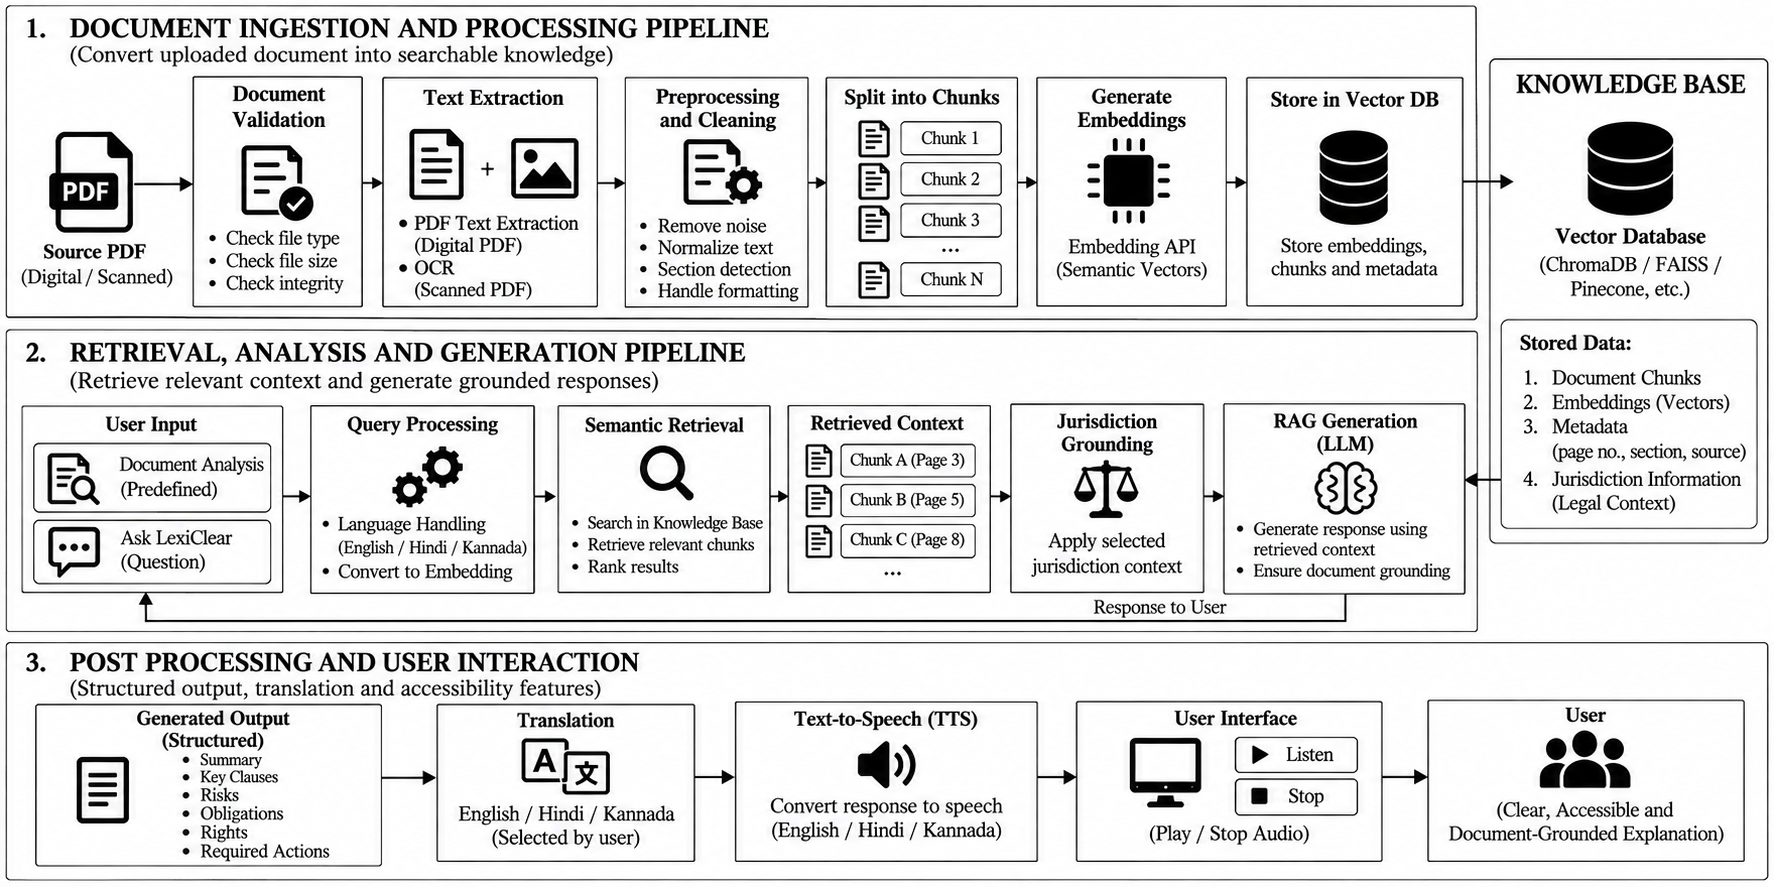
\includegraphics[width=1.0\textwidth]{img.png}
    \caption{Document Processing Pipeline of LexiClear}
    \label{fig:flowchart}
\end{figure}

Figure~\ref{fig:flowchart} describes the proposed system architecture of
LexiClear and illustrates the flow of information from document upload to
the delivery of an accessible, document-grounded response. The architecture
is divided into three major stages: document ingestion and processing,
retrieval, analysis and generation, and post processing and user interaction.
Each stage performs a specific set of operations that together form the
complete document-understanding workflow. The figure provides the
high-level representation of the methodology, while the subsequent sections
describe the individual components and processing operations in greater
detail.

The complete processing strategy is designed to maintain a continuous connection between the uploaded document, the retrieved information, and the final user-facing output. Each stage depends on the result of the preceding stage, allowing the system to progressively transform the original PDF into accessible document information. This sequential design also separates document processing from user interaction, making the individual stages easier to manage and understand. The same processed document representation can support both predefined analysis and user-submitted questions through Ask LexiClear. The final output can then be adapted according to the user's preferred method of access, including structured text, multilingual presentation, or speech output. Thus, the overall strategy provides a unified workflow from document ingestion to information retrieval, response generation, and accessible presentation.

\section{Document Ingestion and Processing}

The document ingestion and processing stage forms the first operational stage
of the proposed LexiClear methodology. The main purpose of this stage is to turn the PDF uploaded by the user into one consistent textual representation that the retrieval and generation components can work with. Legal and administrative documents differ a lot in how they are structured and how they were made. Some contain text that a machine can read directly, while others are made up of scanned pages or embedded images. The methodology therefore has two separate processing paths, direct text extraction and Optical Character Recognition (OCR). Whichever path is used, the text then goes through preprocessing, chunking, embedding and storage, so that the document ends up as a searchable knowledge base. The ingestion stage has a direct effect on everything after it, because semantic retrieval works on the text that this stage creates.

The quality of the ingestion stage directly affects the later stages of the
system because semantic retrieval operates on the textual representation
created during this process. If important information is not extracted, or
if the extracted content contains substantial unwanted artifacts, the
corresponding information may not be represented correctly during embedding
and retrieval. For this reason, document ingestion is treated as more than a
simple file-upload operation. 

\subsection{Document Validation}

The uploaded document first passes through a validation stage before the
remaining processing operations are performed. Validation checks that the input is a supported PDF that the document pipeline can handle. File type, file size and basic file integrity are looked at here. It acts as the first control point in the methodology, stopping unsupported input before it can reach extraction or OCR. It also gives the remaining stages a predictable starting point. Later components expect content that can be extracted or recognized, so checking the input before any processing begins reduces the chance of errors spreading through the pipeline.

Validation does not try to work out what the document means legally or administratively. It only confirms that the document is suitable for processing and can be sent down the right extraction path. It also supports the reliability of ingestion as a whole. A document that could not be processed correctly should never be treated as if it had been converted into a searchable form, and drawing that line means later components only work with documents whose text has really been obtained. In this sense validation marks the boundary between the file the user provides and the internal document-processing pipeline.

\subsection{Document Type Identification}

Once a file has passed validation, we look at it to decide how its text should be obtained. A digitally generated PDF may have selectable, machine-readable text, whereas a scanned or image-based PDF may hold its visible content mostly as images. The two cases need different handling, so LexiClear separates documents that can go through direct text extraction from those that need OCR. The distinction matters because the later stages operate on text and not on how the PDF looks. If machine-readable text exists, it can be extracted without character recognition. If the pages are scans, the visual content has to be converted into text before preprocessing and semantic representation can happen. Identifying the document type also makes the system more flexible. A system that took only machine-readable PDFs would be unable to deal with documents that have been scanned or digitized as images. Supporting both direct extraction and OCR gives LexiClear one methodology for different kinds of PDF input, and once extraction is finished the text moves through the same later stages whichever route it took.

\subsection{Text Extraction and OCR}

For digital documents the system uses direct PDF text extraction, and for scanned or image-based PDFs it uses Optical Character Recognition (OCR). Direct extraction takes the text already embedded in the PDF and hands it to the preprocessing stage with no extra recognition step. This is the right choice when the characters in the document can be accessed by the processing system. The extracted text then serves as the starting point for cleaning, segmentation, chunking and the semantic processing that follows.

OCR is used when the text is stored visually and not as accessible characters. In that case the visual content of the document is analyzed and recognizable characters are converted to machine-readable text. Scanned agreements, notifications, forms and other image-based documents can therefore enter the same downstream pipeline as digitally generated ones. Because of the OCR stage, LexiClear handles more document formats, and users do not have to convert a scanned document into text by hand. OCR output is still just extracted text, so it has to pass through the remaining preprocessing stages like any other. How accurate the recognition is depends on things such as how clear the source document is, the page layout and the quality of the scanned image. Recognition errors may appear in the text and could affect semantic representation and retrieval later on. For that reason the methodology does not count OCR as a full document-understanding step. Its job is to supply the machine-readable text that the rest of the pipeline needs.

\subsection{OCR-Based Processing of Scanned Documents}

Scanned documents need special attention because what the reader sees is stored as images and not as ordinary selectable text. OCR acts as a bridge between that visual representation and the text-based components of LexiClear. Once the
characters have been recognized, the resulting text can be processed using
the same general pipeline applied to digitally generated documents. This
allows the retrieval and generation components to operate without requiring
a separate question-answering architecture for scanned documents.

Because scanned documents end up as ordinary text, the retrieval and generation components can handle them without a separate question-answering architecture. The OCR route starts by recognizing the text on the scanned pages. That recognized text is cleaned and organized before it is divided into chunks, and the order matters: OCR output can carry irregular spacing, stray line breaks and other artifacts that do not match the logical structure of the original document, so the raw recognition result is never treated as the final searchable form. Using OCR also adds a dependency to the workflow. If a character is recognized wrongly, the text we hold may differ from the original, and that difference can reach the embedding and retrieval stages. Scanned documents therefore go through the same later pipeline as digital ones, but their starting text depends on how well OCR performed, and this should be kept in mind when judging the quality and limits of retrieval from scanned material.

\subsection{Text Cleaning and Normalization}

The extracted document content is prepared through preprocessing and
cleaning before it is converted into semantic representations. Raw PDF extraction and OCR can leave behind extra whitespace, broken lines, repeated characters, formatting artifacts and similar oddities. None of these carry real information from the source document, so the preprocessing stage prepares the extracted text to give later operations something more consistent to work with. Normalization supports the same goal across different parts of a document. Spacing, line breaks and other formatting habits often reflect the original layout and say nothing about the content, and tidying them produces cleaner segments for chunking and embedding. We are not trying to rewrite what the document means. The aim is to prepare the text for computational processing while keeping everything later stages need.

Preprocessing also has to preserve information that matters for understanding. Cleaning too aggressively could strip out something that gives a clause its meaning, while cleaning too little leaves artifacts that interfere with semantic representation. We therefore treat preprocessing as a controlled preparation step between extraction and segmentation, and its result is a better basis for dividing the document into searchable units.

\subsection{Document Segmentation}

After the extracted content has been cleaned, the document is organized into
logical portions before the final chunking and embedding stages. Segmentation splits the large body of extracted text into sections of manageable size. A legal or administrative document may hold many clauses, headings, paragraphs, conditions and other structural elements, and keeping useful boundaries in place helps preserve the link between related pieces of information. It is needed because the whole document is usually too big and too general to be a single retrieval unit. The document is broken down step by step into smaller portions that can each be represented and retrieved on their own. This gives later chunking its structural basis, and it keeps each piece of text connected to its position in the source. We want portions that keep useful context without mixing in unrelated material. A section about a particular obligation, condition or clause should stay close enough to its surroundings that retrieval can hand the generation component something meaningful. Segmentation therefore feeds directly into the quality of the searchable representation built from the original PDF.

\subsection{Text Chunking}

The processed document content is divided into smaller chunks so that
individual portions can be represented and retrieved according to a user's
query. A full legal or administrative document can run to many pages and cover several unrelated topics, and treating all of it as one retrieval unit would make it hard to isolate what a particular question is about. Smaller chunks give more focused units for semantic representation and retrieval. Each one is a searchable unit in the document knowledge base, so when a question arrives the retrieval component can pick out the chunks whose content relates to it instead of returning the whole document, which cuts down the irrelevant material passed on to generation. At the same time, a chunk has to keep enough context to be useful once it reaches the RAG component.

Chunk size is a balance between specificity and context. If chunks are too large, retrieval may bring back a lot of unrelated text, and if they are too small, important relationships may be split across several units. We treat chunking as a key preparation stage for semantic retrieval, and the chunks it produces are the basic text units from which embeddings and searchable representations are made.

\subsection{Semantic Embedding Generation}

After chunking, each document chunk is converted into a semantic vector
using an embedding API. An embedding represents the textual content in a
numerical form that can be compared with other text representations. This
allows the retrieval stage to compare the representation of a user query
with the representations of document chunks. The embedding stage therefore
creates the connection between the textual document content and the
semantic retrieval mechanism used later in the methodology.

The embedding representation is generated for each processed chunk rather
than for the entire document as a single unit. This allows the retrieval
system to identify specific portions of the document that are related to a
user's information requirement. The semantic representation is therefore
closely connected to the chunking stage: chunking determines the units of
information, while embedding converts those units into representations that
can participate in similarity-based retrieval.

The generated embeddings do not replace the original document text. The
textual chunk remains available as the source content associated with its
vector representation. This distinction is important because the embedding
provides a mechanism for identifying relevant information, while the
retrieved textual content is later supplied to the analysis and generation
components. The embedding stage therefore supports retrieval without
becoming a substitute for the source document itself.

\subsection{Vector Database Storage}

The generated embeddings, document chunks, and associated metadata are
stored in a vector database. The vector database provides the searchable
storage layer required by the semantic retrieval component. Instead of
searching through the original PDF directly for every user question, the
system can search the processed vector representation and identify document
chunks that are semantically related to the query. This provides an
efficient connection between document ingestion and later user interaction.

Each stored representation maintains a relationship between the semantic
vector and the corresponding document content. This allows the retrieval
stage to identify a relevant vector and then obtain the associated textual
chunk for use as contextual information. Metadata can also be associated
with the stored information so that retrieved content remains connected to
the source document and its processing context.

Vector storage also allows the processed document representation to be used
for multiple interactions. Once the document has been ingested and its
chunks have been embedded and stored, different questions can be submitted
against the same knowledge base without repeating the complete ingestion
process. This supports the interactive nature of LexiClear, where users may
ask multiple questions about the same uploaded document through Ask
LexiClear.

\subsection{Metadata Association}

Along with the document chunks and their semantic representations, relevant
metadata is associated with the stored information. Metadata records how each stored chunk relates to its source document. Keeping that link matters because the semantic vector on its own does not contain the full text that must eventually go to the generation component. Metadata also helps organize information inside the processed document. When a relevant chunk is retrieved, the system can keep it tied to the matching document content and does not have to treat it as an isolated snippet. That fits document-oriented interaction well, since retrieval is meant to return material from the user's own uploaded document and not unrelated general information. Metadata is part of the knowledge representation created during ingestion. Together with the original document, the processed text, the chunks and the embeddings, it makes up what the retrieval stage needs. Ingestion is complete once this searchable representation has been created and stored where later analysis and generation components can reach it.

The processed content is cleaned and normalized, organized into segments and then split into smaller chunks. These chunks are converted into semantic embeddings and kept in the vector database along with their text and metadata. Each stage helps turn the original PDF into a representation that supports semantic retrieval later on. This workflow also draws a clear line between processing the source document and processing the user's query. During ingestion, the system concentrates on preparing the document and creating its searchable representation.

\subsection{Document Processing Workflow}

The complete document ingestion process can therefore be represented as a
sequence beginning with document upload and validation, followed by document
type identification and text extraction or OCR. Afterwards, the system uses that stored representation to answer questions without going through the whole document-processing routine again. Keeping the two apart makes the methodology easier to organize and lets one processed document support many analysis and question-answering operations. What ingestion produces is not an answer. It is a searchable knowledge representation of the uploaded document, holding the processed content in a form that can be compared against future user queries. The next stage, Retrieval, Analysis and Generation, uses it to find relevant information, add contextual information and generate responses. Document
ingestion thus provides the technical foundation on which the remainder of
the LexiClear methodology operates.

\section{Retrieval, Analysis and Generation}

The second stage handles both predefined document analysis and questions
submitted through Ask LexiClear. Once the document has been processed and stored in the knowledge base, LexiClear can respond to what a user needs without reprocessing the original PDF from scratch. The user's input is handled according to the selected language, and the query is converted into an embedding. Semantic retrieval then runs against the stored document embeddings, finding and ranking the chunks that are most relevant to the query. This stage is what links the user's need to the content of the uploaded document. Users do not have to hunt for the right terms or clauses, because the retrieval component finds content that is semantically related to what they asked. The retrieved chunks supply the context for the analysis and generation components. Keeping retrieval and generation separate matters here, because it lets the system identify the source information first and only then ask the language model to compose the final response.

Semantic retrieval picks out chunks according to how similar their context is to the query, instead of relying only on exact keywords. This helps most when the user's wording differs from the formal terminology in the document: a person may describe an idea in everyday language while the matching provision uses a formal or domain-specific expression. Retrieval therefore works as a middle layer between natural-language interaction and the document's content. After the query has been represented semantically, the mechanism finds the segments related to it and passes them on as context for analysis and response generation. It does not write the final explanation itself. It supplies the relevant source content to the components that do.

\subsection{Semantic Retrieval}

The user's input is converted into an embedding representation and compared
with the stored document embeddings. The post-processing stage covers structured document analysis, summary generation, identification of important clauses and information, interactive question answering through Ask LexiClear, multilingual translation and text-to-speech conversion. All of these work on information drawn from the uploaded document and from the retrieval and generation stages. They are connected so that a user can start from a general understanding of the document and move on to more specific questions or other ways of accessing the generated information.

\subsection{Jurisdiction Grounding}

The retrieved context is passed to the jurisdiction grounding component,
where the selected jurisdictional context is incorporated into the analysis.
The jurisdictional information provides an additional contextual layer for
legal or administrative information that may vary according to the selected
jurisdiction. This stage is intended to help frame the generated
information within the jurisdiction selected or configured for the system
rather than treating all legal information as universally applicable.

The jurisdictional context is used to guide the response rather than being
treated as a replacement for the information contained in the uploaded
document. The uploaded document remains the primary source of
document-specific information, while jurisdictional information provides
additional context for interpreting or presenting that information. The
quality of this stage therefore depends on the quality and coverage of the
configured contextual information. Jurisdiction grounding is consequently
treated as a contextual support mechanism within the methodology rather
than as an independent source of authoritative legal interpretation.

\subsection{Retrieval-Augmented Generation}

The resulting contextual information is provided to the
Retrieval-Augmented Generation (RAG) component. The RAG component uses the
retrieved document content and jurisdictional context to generate a grounded
response. Instead of producing an answer independently of the uploaded
document, the generation stage receives relevant document information as
context. This creates a direct connection between the retrieval stage and
the natural-language response delivered to the user.

This approach helps maintain a connection between the generated response and
the information contained in the uploaded document. It also allows the
system to respond to questions where the terminology used by the user may
differ from the exact wording present in the document. The retrieved chunks
provide the information required for the response, while the language model
converts that information into a natural-language explanation. The generated
response can then be passed to the post-processing components for structured
presentation, translation, or speech-based access.

\section{Post Processing and User Interaction}

The final stage of the LexiClear methodology is responsible for converting the information generated from the retrieval and analysis pipeline into an accessible and understandable form for the user. While the earlier stages focus primarily on document processing, retrieval, contextual grounding, and response generation, this stage focuses on how the resulting information is organized, presented, translated, and delivered. The purpose of post processing is therefore not only to display the generated response but also to transform it into different forms that support easier comprehension and interaction with the processed document.

The post processing stage consists of structured document analysis, summary generation, identification of important clauses and information, interactive question answering through Ask LexiClear, multilingual translation, and text-to-speech conversion. These functions operate on the information obtained from the uploaded document and the retrieval and generation stages. The different components are connected so that the user can move from a general understanding of the document to more specific questions and alternative forms of accessing the generated information.

\subsection{Structured Document Analysis}

Structured analysis sorts the information taken from the document into meaningful categories. Rather than showing everything as one continuous block of generated text, LexiClear separates the important aspects of the document by the role they play. A user can then look at one kind of information without combing through the whole document. The categories include summary, key clauses, risks, obligations, rights, conditions and required actions. Each gives a different view of the same document and helps the user grasp both its general meaning and its practical consequences. The structure also gives a consistent output format across the different documents the system handles. All of this is generated from information that came through the document-processing and retrieval pipeline, so the uploaded document remains the main source of anything document-specific.

\subsection{Summary Generation}

A summary gives a short version of the main information in the uploaded document. Legal and administrative documents can run to several pages of formal text with definitions, conditions, exceptions, responsibilities and supporting clauses, and reading all of it takes time, especially for someone who only wants to know what the document is about. LexiClear uses the processed document information to produce a simplified summary that brings out the central content. It is meant to give an initial understanding before the user looks at specific clauses or asks detailed questions, and it can describe the general purpose of the document, the main parties or entities involved, important responsibilities and other relevant details found in the processed content. Users can take the summary as an overview and then go to specific sections, clauses or questions when they need more detail. That way the system supports quick understanding as well as deeper exploration.

\subsection{Key Clause Identification}

Key clause identification finds and presents the clauses that carry important document-specific information. In legal and administrative documents, conditions, responsibilities, restrictions, exceptions and procedural requirements are often scattered across different parts, and pointing them out helps users put their attention where a closer look may be needed. Clauses are organized according to what the document analysis identified. A key clause might describe an obligation that has to be met, a condition that changes how an agreement applies, a restriction on some action or another significant requirement. Presenting these clauses separately makes the output more useful than presenting only a general summary. The identified clauses remain connected to the information retrieved from the uploaded document. This allows the structured output to remain document-specific while providing a more accessible representation of the original content. The user can consequently use the identified clauses as entry points for further examination or for asking questions through Ask LexiClear.

\subsection{Rights and Obligations}

Rights and obligations represent another important category of structured document information. Formal documents may describe what a party is permitted to do, what a party is required to do, and what conditions govern those responsibilities. Such information can be difficult to locate when it is embedded within long paragraphs or presented using formal terminology. LexiClear organizes relevant information into rights and obligations so that users can distinguish between permitted actions and required responsibilities. The system can present these elements in a more understandable form while maintaining their relationship with the information contained in the uploaded document. This organization is particularly useful when a document contains responsibilities for multiple parties.

The purpose of this component is to make important responsibilities more visible rather than requiring the user to identify them manually from the complete document. The resulting information can also provide useful context for subsequent questions. If the user requires clarification about a particular obligation or right, the Ask LexiClear component can be used to retrieve and explain the relevant document information.

\subsection{Risks and Conditions}

Risks and conditions provide a separate view of information that may affect how the document applies in particular situations. Conditions may say when an obligation starts to apply, when a service or agreement can be changed, or what circumstances could lead to a particular action. This kind of information often sits across several clauses and is easy to miss on a quick read. LexiClear gathers the relevant conditions and related details into a dedicated part of the structured output, so users can examine the circumstances, restrictions and dependencies that might affect how the document is interpreted. When the relevant information is spread over several retrieved chunks, the retrieval and generation workflow supplies the context needed to show it together. The structured presentation of risks and conditions does not decide the legal effect of a clause. It is an accessible representation of what is in the processed document. Users can treat it as a starting point and go back to the original document when precise interpretation is needed.

\subsection{Required Actions}

Required actions identify practical steps or responsibilities that are described in the uploaded document. Many administrative and formal documents contain instructions that require a party to perform a particular action within specified conditions. These actions may be easier for a user to understand when they are separated from descriptive or background information.

LexiClear organizes relevant action-oriented information so that users can identify what needs to be done based on the processed document content. The generated representation may include actions, responsibilities, or procedural requirements that are explicitly described in the document. This turns long formal descriptions into something a reader can look at from a practical angle. The required-actions category works hand in hand with rights, obligations, conditions and key clauses, since each gives a different view of the same document. An obligation may state a responsibility, a condition may say when it applies, and the required action says what actually has to be done. Laying these relationships out clearly makes the generated analysis easier to read.

\subsection{Ask LexiClear}

Ask LexiClear is the interactive question-answering interface where users can put questions about the uploaded document. It sits as an interactive layer on top of the knowledge representation built during the earlier processing stages. A submitted question goes through the retrieval workflow: the system processes it, generates its semantic representation and finds the document chunks that match. Those chunks are handed to the generation component together with the appropriate contextual information, and the response comes back as an explanation based on the processed document. Ask LexiClear can be used after the structured analysis or entirely on its own for specific questions. A user might read the summary first, for instance, and then ask about one particular obligation, condition, clause or required action. 

\subsection{Document-Specific Question Answering}

Document-specific question answering ensures that user queries are interpreted in relation to the uploaded document rather than being treated as unrestricted general questions. This distinction is important because the purpose of LexiClear is to help users understand the content of a particular legal or administrative document.

The retrieval stage identifies the portions of the uploaded document that are most relevant to the user's question. These retrieved sections provide the context used by the RAG component when generating the response. Consequently, the answer is connected to the information available in the processed document instead of depending only on the wording of the question. The question-answering workflow also allows users to investigate information that may not be emphasized in the initial structured analysis. A user can ask about a specific clause, condition, responsibility, deadline, or other document-related topic and receive a response based on the relevant retrieved context. This makes the interaction more flexible than a fixed document-summary interface.

\subsection{Interactive Follow-Up Questions}

The interactive nature of Ask LexiClear allows users to progressively explore a document. A user may begin with a broad question and subsequently ask more specific questions based on the response received. This creates a conversational method of navigating document information without requiring the user to repeatedly search through the complete PDF. Follow-up questions can be used to examine particular parts of the document in greater detail. For example, after identifying an obligation through the structured analysis, the user may ask what conditions are associated with that obligation or what action is described in the relevant clause. That lets one workflow support both an overview of the document and targeted questions about it.

Every question runs through the retrieval and generation workflow so that the relevant document context ends up in the response. This helps most with long documents, where it saves users from paging through the file by hand. The interactive component does not replace the original document. It offers one more way to find and understand what the document contains.

\subsection{Multilingual Translation}

Multilingual translation makes LexiClear more accessible by presenting generated responses in several languages. The implemented system lets users choose English, Hindi or Kannada as the output language. The idea is to help people who would rather read an explanation in a language other than English, particularly when it concerns a formal document. Translation acts on the response produced by the document-understanding workflow. The uploaded document stays the primary source of document-specific information, and translation only changes the language in which the explanation appears, which keeps the source document distinct from the accessibility-oriented output the system generates. This helps especially when the original is written in formal English that some users find hard to follow. Giving the explanation in the chosen language lowers that barrier while keeping the main points found during analysis.

\subsection{Language Selection}

The user can select the preferred output language according to the supported language options provided by the system. The selected language determines the language used for the generated or translated response presented through the interface. This allows the same document-processing and retrieval workflow to serve users with different language preferences.

Language selection is applied after the relevant document information has been identified and the response has been generated. This design separates document understanding from language presentation. The system can therefore retrieve and analyze document content before presenting the resulting explanation in the language selected by the user. The language-selection functionality also provides a consistent interaction model across the different output modes. A user can obtain a response in English, Hindi, or Kannada and can subsequently use the text-to-speech component to listen to the response where speech output is supported. This creates a connection between multilingual text accessibility and audio-based accessibility.

\subsection{Text-to-Speech}

Text-to-speech functionality provides an audio representation of the generated response. Instead of requiring the user to read the complete explanation, the system can convert the displayed response into speech. This provides an additional method of accessing information and supports users who prefer auditory interaction with the generated content. The text-to-speech component can operate on the generated or translated response presented by LexiClear. This means that the speech output can be associated with the language selected by the user when supported by the speech-processing component. The feature therefore connects the multilingual output stage with an alternative audio-based presentation method.

The text-to-speech functionality is designed as an accessibility feature rather than as a separate document-processing mechanism. The underlying document remains unchanged, while the generated explanation is converted into an audio form for easier consumption. This allows users to choose between reading the response and listening to it according to their preferred interaction method.

\subsection{Audio Interaction Controls}

The LexiClear user interface provides Listen and Stop controls for interacting with the text-to-speech output. The Listen control starts speech playback of the generated response, and the Stop control ends it whenever the user wants. Because the controls sit in the interface itself, users do not need a separate speech application. They are tied to the response shown on screen: when a user asks for speech, the selected response is passed to the text-to-speech component and the audio is made available through the interface. Stop is useful when someone wants to go back to reading or move on to another action on the document. Text-to-speech was demonstrated as part of the implemented system, including speech output for Kannada responses. At this stage the methodology is concerned with integrating speech accessibility into the document-understanding workflow, not with a quantitative evaluation of speech quality. The audio component is another accessibility layer attached to the multilingual response-generation process.

\subsection{Integration of Post Processing Components}

The different post processing components operate as connected parts of a single user interaction workflow. Structured analysis provides an organized representation of document information, Ask LexiClear provides interactive access to specific information, multilingual translation changes the language of the generated response, and text-to-speech provides an audio representation of that response.

The components can be used together depending on the user's requirements. A user may first obtain a structured summary, ask a question about a particular clause, select a preferred language, and then listen to the resulting response. This sequence allows LexiClear to support multiple forms of document access without requiring separate systems for each interaction type. The integration of these components ensures that the output stage remains connected to the earlier document-processing and retrieval stages. The information presented to the user originates from the processed document and retrieved context, while the post processing components determine how that information is organized and delivered. In this way, the final stage completes the transformation from a complex PDF document into an interactive and accessible form of document understanding.
\section{End-to-End System Workflow}

The complete LexiClear workflow begins when the user uploads a legal or
administrative PDF document. A document is first validated and then processed through direct text extraction or OCR, depending on its format. The extracted content is cleaned, divided into meaningful chunks, converted into semantic embeddings and stored in the vector database along with relevant metadata. This first part of the workflow builds the searchable representation of the uploaded document and gets its information ready for retrieval. The document itself is still the primary source of the content used in later analysis and response generation.

When the user asks for analysis or submits a question through Ask LexiClear, the system retrieves relevant chunks using semantic retrieval. That information is combined with the selected jurisdictional context and sent to the RAG component, which generates a document-grounded response. This is the stage that connects what the user needs with the processed representation of the document. Users do not have to find the passages themselves, because the retrieval mechanism finds them and passes them to the generation component as context. The response is then organized into structured information where needed and can be translated into English, Hindi or Kannada. It can also be converted into speech and played through the Listen and Stop controls in the interface. These post-processing features are different ways of reaching the same document-grounded information. In this end-to-end workflow, LexiClear brings document processing, retrieval, generation, contextual grounding, multilingual processing and speech accessibility together in one system.

The methodology can therefore be viewed as a sequence of connected
transformations in which the original PDF is progressively converted into
searchable document information, relevant contextual information, a
generated explanation, and finally an accessible user-facing response. The
different stages are dependent on one another: document processing provides
the content required for retrieval, retrieval provides the context required
for generation, and post processing provides the mechanisms through which
the generated information can be accessed. This organization ensures that
the system does not treat document processing, question answering,
translation, and speech interaction as isolated features, but as components
of a common document-understanding workflow.

\chapter{Results}

The development of LexiClear resulted in an integrated prototype for processing legal and administrative documents and presenting their information in an accessible form. The implemented workflow combines document ingestion, text extraction, OCR support, semantic retrieval, Retrieval-Augmented Generation, jurisdiction grounding, structured analysis, multilingual translation, and text-to-speech functionality. The system was tested through backend and frontend integration to verify the operation of the major components. The results presented in this chapter focus primarily on the functional behavior of the developed system. We have not yet built a large expert-labelled dataset or set up a controlled quantitative evaluation. For that reason the results below are described through the available document inputs, the experimental setup and functional observations, and no numerical accuracy or performance figures are claimed.

\section{Dataset}

LexiClear is built to process legal and administrative PDFs in general and does not depend on one fixed dataset. For development and functional evaluation we therefore chose documents that stand for the different kinds of legal and administrative information a user might need to understand. They contain clauses, conditions, obligations, rights, responsibilities, financial terms, restrictions and other content relevant to document-based analysis and question answering.

Three legal documents were used to represent different document-understanding scenarios: an employment-related legal document, a Simple Mortgage Deed and a Leave and License Agreement. We picked them because each mixes structured and unstructured legal information, which gives a good basis for testing document processing, semantic retrieval, document analysis and question answering. The employment-related document stands for the kind of paperwork in which users need to understand employment conditions, responsibilities, contractual requirements and related clauses, and its formal terminology can be hard going for non-experts. The Simple Mortgage Deed is a financial and property-related document that carries financial obligations, conditions, rights and restrictions. The Leave and
License Agreement represents an agreement-oriented document containing
information related to the parties involved, terms and conditions, permitted
use, responsibilities, restrictions, and other contractual provisions.

Using more than one document means the workflow can be looked at across different document structures and not just one type of legal text. This matters because the system is meant to work on whatever documents users upload, so the pipeline has to cope with differences in structure, terminology, clause organization and information density.

\subsection{Question-Answer Dataset}

To evaluate Ask LexiClear, we prepared question-answer datasets in CSV format from the documents used in testing. Every CSV file has two fields, question and expected\_answer. The question field holds a document-specific question, and expected\_answer holds the information we expected the system to return, taken from the source document. The questions test whether LexiClear can retrieve and give back information about specific clauses, conditions and details in the source, and so the generated response can be compared with what the source material says it should be.

We prepared three separate CSV files, one for each document used in functional testing. The first, qa\_test.csv, has 20 question-answer pairs based on the employment-related legal document. The second, mortgage\_deed\_qa\_test.csv, has 20 pairs based on the Simple Mortgage Deed, and the third, leave\_license\_agreement\_qa\_test.csv, has 20 pairs based on the Leave and License Agreement. In total that gives 60 document-specific question-answer pairs for the functional evaluation of the document question-answering workflow.

The datasets are meant to check whether the system can locate information in the uploaded document and generate a response that matches what was asked. They are not a formally curated legal benchmark, nor an expert-created dataset for judging legal interpretation. They are a controlled set of document-specific queries used to look at how the retrieval and generation pipeline behaves.

The chosen documents cover contractual and agreement-style content along with financial and employment-related conditions, so the terminology and types of information vary. The question-answer pairs are document-specific as well. We did not ask general legal questions; each question is tied to the contents of its own uploaded document. This is important because Ask LexiClear exists to let users interact with their own documents and get information grounded in them. The dataset can be seen as having two linked parts: the source legal documents, which supply the information to be processed and retrieved, and the questions with expected answers, which give a basis for evaluating the question-answering behaviour of the system.

\subsection{Document Representation for Retrieval}

The documents used for evaluation are processed through the same document
ingestion pipeline implemented in LexiClear. The system supports both
machine-readable digital PDFs and scanned or image-based PDF documents. For
digital documents, text can be extracted directly from the PDF, while OCR is
used when the document contains scanned or image-based content. After text extraction, the document content is subjected to preprocessing and
is divided into smaller meaningful chunks. Chunking allows lengthy documents
to be represented as smaller retrievable units rather than requiring the
complete document to be supplied during every retrieval operation. Each
processed chunk is converted into a semantic embedding and stored together
with relevant metadata.

The metadata associated with document chunks can include information such as
the source document, page number, section, and other available
document-location details. This information provides additional context for
the retrieval process and helps maintain a connection between the generated
response and the original document. The resulting representation forms the searchable knowledge base used by the
semantic retrieval and Retrieval-Augmented Generation (RAG) components.
When a user submits a question through Ask LexiClear, the question is
processed into a semantic representation and compared with the stored
document representations. Relevant document chunks can then be retrieved and
provided as contextual information for response generation.

\subsection{Dataset Characteristics}

The dataset contains documents representing different categories of legal and
administrative information. The selected documents include both contractual
and agreement-oriented content as well as information involving financial and
employment-related conditions. This provides variation in the terminology and
types of information that may be encountered during document processing and
question answering.

The question-answer pairs are also document-specific. Rather than asking
general legal questions, the evaluation questions are associated with the
contents of the corresponding uploaded document. This distinction is
important because the primary purpose of Ask LexiClear is to allow users to
interact with their own documents and obtain information grounded in those
documents. The dataset can therefore be viewed as consisting of two connected
components. The first component is the collection of source legal documents,
which provides the information to be processed and retrieved. The second
component is the set of document-specific questions and expected answers,
which provides a basis for evaluating the question-answering behaviour of the
system.

\subsection{Purpose of the Dataset}

The primary purpose of the dataset is to support functional and
document-oriented evaluation of the LexiClear pipeline. The selected
documents provide input for testing document upload, extraction,
preprocessing, chunking, semantic representation, retrieval, and
document-grounded response generation. The associated question-answer pairs
provide queries through which the retrieval and question-answering components
can be examined.

The dataset also supports evaluation of the overall interaction between the
document-processing and response-generation components. A successful
question-answering interaction requires the system to process the source
document, create a searchable representation, identify relevant information
for the submitted question, and generate a response based on the retrieved
content. The expected answers are derived from the corresponding source documents and
are therefore used as reference information during evaluation. They should
not, however, be interpreted as expert-annotated ground truth for legal
interpretation. The evaluation focuses on whether the system can retrieve and
present information from the tested documents rather than whether it can
establish the legal validity or authoritative interpretation of a provision.

\subsection{Dataset Limitations}

The dataset has several limitations that should be considered when
interpreting the results. There are some limitations. First, only three source documents were used for development and functional evaluation. They stand for different legal scenarios, but they cannot cover the full range of legal and administrative documents found in real use. Second, the question-answer datasets were written specifically from the test documents, so the questions are document-specific and do not make up a large independent benchmark. The expected answers are information extracted from the documents and are not expert-annotated labels of legal correctness. Third, the dataset does not give a controlled evaluation of every document characteristic. Document length, formatting complexity, OCR quality, variation in terminology and clause structure can all affect retrieval and generation. A larger dataset with documents from a wider range of legal and administrative categories would give a firmer basis for judging general behaviour. Finally, the dataset is mainly meant for functional evaluation of the LexiClear workflow, so results from these documents and questions should be read within the scope of the tested set. They are not a general measure of legal accuracy, and they are not evidence that the system can carry out authoritative legal interpretation on its own.

\section{Experimental Setup}

The experimental setup consists of the major software components required to
implement and test the LexiClear workflow. The system follows a client-server
architecture in which the frontend provides the user interface and communicates
with the backend through defined endpoints. This arrangement separates the
user interaction layer from the document-processing and AI-based processing
components, allowing the different stages of the system to operate as an
integrated workflow.

The frontend is implemented using React with Vite. The frontend is the interface through which users upload legal or administrative documents, view the generated analysis, use Ask LexiClear, select the output language and control speech playback. It is the main layer of interaction between the user and the document-processing pipeline underneath. The backend is implemented with FastAPI and handles document upload, document processing, analysis requests, question answering, translation-related operations and speech-generation requests. It also connects the application interface to the document-processing, retrieval and generation components needed to produce document-grounded responses.

The experimental workflow starts when a legal or administrative PDF is uploaded through the frontend. The document is validated and then passed to the document-processing pipeline. Depending on its type, text is obtained either by direct PDF text extraction or by Optical Character Recognition (OCR) for scanned or image-based files, so the same workflow can take both machine-readable and image-based PDFs. After extraction, the content is preprocessed and divided into smaller chunks, which gives manageable units that can be retrieved when a user asks something. The chunks are converted into semantic embeddings and stored with document-related information, and this becomes the searchable knowledge base used by the semantic retrieval and Retrieval-Augmented Generation (RAG) components.

For document analysis, the processed document goes through the retrieval and generation workflow to collect the information the analysis request needs. The result is organized, where it applies, into structured categories including summary, key clauses, risks, obligations, rights and required actions. Users see this structured view in the frontend and do not have to go through the whole source document manually. For the Ask LexiClear evaluation, a document-specific question is submitted through the user interface.

The Kannada text-to-speech feature was tested during development as well. The system successfully generated a WAV audio file from a generated legal statement, using the Apple MPS device configuration that was available. The experimental setup therefore checked the major components both on their own and together as one workflow. The verification scenarios covered document upload, document processing, document analysis, document-specific question answering, language selection, Kannada speech generation, audio playback controls and jurisdiction grounding. Together they show that the implemented components can communicate with each other and work as part of the complete LexiClear system. The evaluation concentrates on functional behaviour and on how well the components integrate. The question is processed and represented
semantically before relevant document chunks are retrieved from the
knowledge base. The retrieved content is then supplied to the RAG generation
component as contextual information. Jurisdictional information can also be
incorporated into this workflow when the corresponding functionality is used.
The generated response is therefore produced within the context of the
uploaded document and the selected configuration.

The generated response can subsequently be processed according to the
selected output language. LexiClear supports English, Hindi, and Kannada
output. The translation operation is applied to the generated response while
the uploaded document remains the primary source of the document-specific
information. This allows the same document-grounded response to be presented
through different language options.

Speech generation was also included as part of the experimental setup. When
speech output is requested, the generated or translated response is passed to
the text-to-speech component. The frontend provides Listen and Stop controls
for interacting with the generated audio. This allows the speech functionality
to be tested as an integrated part of the overall document-understanding and
accessibility workflow.

Development and integration testing were performed in a macOS environment.
The backend document-analysis endpoint was tested using a rental agreement and
successfully returned structured analysis for the document content. The
frontend was connected to the document upload, analysis, Ask LexiClear, and
speech-related interactions. The Kannada text-to-speech functionality was
also tested during development, where the system successfully generated a WAV
audio file from a generated legal statement using the available Apple MPS
device configuration.

The experimental setup was therefore used to verify the operation of the
major components both individually and as an integrated workflow. The
verification scenarios covered document upload, document processing, document
analysis, document-specific question answering, language selection, Kannada
speech generation, audio playback controls, and jurisdiction grounding. These
scenarios provide functional evidence that the implemented components can
communicate with each other and operate as part of the complete LexiClear
system.

The experimental evaluation is primarily focused on functional behaviour and
integration of the implemented components. Our testing is not a controlled large-scale benchmark of legal accuracy or system performance. The functional observations show that the operations can be carried out successfully, but they do not establish that the generated interpretations are legally correct. The results should therefore be read within the scope of the documents, questions, configurations and testing environment used during development.

\section{Results and Discussions}

The developed LexiClear system was evaluated through functional testing of its major components and their integration into the complete document-understanding workflow. The evaluation focused on verifying whether the system could accept legal documents, process their contents, retrieve relevant information, generate document-grounded responses, and provide multilingual and speech-based accessibility features. The results indicate that the major components of the proposed system have been successfully integrated and can operate as a connected workflow.

\subsection{Document Processing Results}
The document ingestion workflow was tested using legal PDF documents, including a rental agreement. The system accepted the document through the upload interface and passed it to the backend for processing. The pipeline extracts text from digital PDFs and uses OCR for scanned or image-based ones. Once the text is out, it is preprocessed and divided into smaller chunks, and those chunks are converted into semantic embeddings and stored with relevant metadata for later retrieval. The result is the searchable knowledge representation that the retrieval and RAG components depend on. In functional terms, this shows that LexiClear can turn an uploaded legal document into something that can be processed and searched semantically, so users no longer have to find the relevant clauses by hand.

The quality of every later step depends on how well the original document is converted into a machine-processable form. Legal and administrative documents contain long paragraphs, clause numbers, headings, tables and other formatting structures, so pulling out raw text is not enough to support document-specific retrieval. Preprocessing produces the intermediate representation that retrieval and generation then use. Supporting both direct extraction and OCR also means the workflow suits different kinds of PDF. Digitally generated files give text that can be taken out directly, while scanned documents need OCR first, and that matters for legal paperwork because the files people receive do not follow a single format.

Chunking then divides the processed document into smaller units that can each be linked to a semantic representation. Instead of treating the whole document as one large input, the system builds smaller searchable units that can be retrieved for a user's query. The metadata attached to them records where the retrieved content came from, which supports document-specific processing and makes the retrieval workflow easier to trace. Seen end to end, this processing result lays the foundation for the RAG pipeline: a successfully processed document becomes a searchable representation, and later questions can be matched against portions of it. It is the link between the upload step the user sees and the retrieval and question-answering features of LexiClear. The results at this stage are functional and are not accuracy figures. The current evaluation verifies that documents can be accepted, processed, represented, and made available for semantic retrieval, but it does not provide a separately measured extraction accuracy or OCR accuracy score. Such measurements would require a controlled dataset containing documents with verified ground-truth text. Therefore, the present results demonstrate successful integration of the document-processing workflow while leaving detailed extraction and OCR accuracy evaluation for future work.

\begin{figure}[h]
    \centering
    
\includegraphics[width=\textwidth]{lexiclear_homepage.jpg}
    \caption{LexiClear User Interface for Document Analysis}
    \label{fig:lexiclear_interface}
\end{figure}

Figure~\ref{fig:lexiclear_interface} describes the implemented LexiClear user interface for document analysis. The interface provides the entry point for uploading supported documents and accessing the system's analysis workflow. It also presents the major accessibility-oriented capabilities of the system, including summaries, risk signals, plain-language explanations, and voice-based responses.


\subsection{Document Analysis Results}
The document-analysis functionality was tested using a rental agreement. The backend analysis endpoint successfully returned structured information from the document. The generated output organizes relevant information into categories such as summary, key clauses, risks, obligations, rights, and required actions, where applicable. This structured representation provides a more organized alternative to presenting the user with the complete original document. It allows important information to be accessed according to its type and reduces the need to manually examine every section of a lengthy document.

The structured analysis also demonstrates the role of the system beyond simple document retrieval. While retrieval provides relevant portions of the source document in response to a query, document analysis organizes information into predefined categories that are easier for a user to interpret. This is useful for legal and administrative documents because important information often sits across several clauses and is not available in one ready-made summary. The analysis output turns the original formal document into something closer to what a user needs. Obligations and required actions can be shown apart from the general summary, so users can concentrate on one aspect of the agreement. Key clauses and potential risks, in the same way, give a structured view of information that the user would otherwise have to dig out by reading the document.

The rental agreement test also showed how document processing and document analysis depend on each other. Analysis can only run after the document has been uploaded and processed, since the extracted content is what gets passed to the analysis component. That confirms the analysis feature is tied into the earlier stages of the LexiClear pipeline and does not work in isolation. The categories it produces should still be read as system-generated assistance and not as legal conclusions. Seeing a clause listed under a particular category does not mean it is legally valid, unlawful or applicable in every situation. What the testing shows is that LexiClear can organize and explain document information. Authoritative legal interpretation was outside the scope of our evaluation.

Consistency of presentation is another useful result. A structured analysis interface gives different documents a common format even though their contents differ, which can lower the effort needed to spot important information and supports our wider goal of making formal documents easier to understand. This evaluation of document analysis is again functional. We did not use independent expert annotation to measure whether every extracted category was correct or whether each identified risk, obligation or action was legally complete. The result shows that structured document information is generated and presented successfully, but it does not give a quantitative measure of legal-analysis accuracy. Evaluating with expert-labelled documents in future could assess the accuracy and completeness of these categories more systematically. Until then, the generated analysis should be treated as an aid for finding information and understanding documents. The system does not establish the legal validity or authoritative interpretation of the provisions it identifies.

\subsection{Retrieval and RAG Results}

The Retrieval-Augmented Generation (RAG) pipeline was evaluated using 80 document-specific question-answer pairs. The evaluation considered retrieval quality, contextual coverage, generation grounding, and answer relevance. The RAG-specific metrics included Context Relevance, Context Precision, Context Recall, Faithfulness, and Answer Relevance. The RAG evaluation provides a more detailed assessment of the interaction between document retrieval and response generation. In a document-grounded system such as LexiClear, retrieving information that is related to the user's question is an important intermediate step because the generated response depends on the context supplied to the language model. Consequently, retrieval quality and generation quality need to be considered as related but distinct aspects of the overall workflow.

Context Precision provides information about the quality of the retrieved context in relation to the information required for the question. A high value indicates that the retrieved context contains a relatively large proportion of information that is useful for the evaluated query. Context Relevance provides a complementary view by examining how closely the retrieved information corresponds to the submitted question. Considering both measures is useful because a retrieval result may contain relevant information while still including additional content that is not directly required for answering the query. Context Recall represents another important aspect of retrieval performance. It considers whether the information required for answering a question is sufficiently covered by the retrieved context. This is particularly relevant for legal documents because an answer may depend on information distributed across different clauses or sections. If important information is not retrieved, the generation component may not have sufficient source material even when the language model itself is capable of producing a coherent response.

Faithfulness evaluates the relationship between the generated response and the retrieved context. For LexiClear, this is an important consideration because the purpose of the RAG workflow is to generate answers based on the uploaded document rather than relying solely on general language-model knowledge. A response that is fluent but insufficiently grounded in the retrieved document would not fully satisfy the document-understanding objective of the system. Answer Relevance provides a user-oriented view of the generated response by measuring how directly the response addresses the submitted question. This complements the retrieval-oriented metrics because a response may be grounded in the retrieved context while still not directly addressing what the user asked. Examining retrieval and answer metrics together therefore provides a broader understanding of the behaviour of the RAG pipeline.

The aggregate results should also be interpreted together with the per-question visualizations presented later in this section. An average metric provides a summary of the evaluation set, but it does not show whether the measured behaviour is consistent across individual questions. The heatmap and individual-question graphs therefore provide additional information about variation within the 80-question evaluation set. The differences between individual questions can arise from the nature of the question, the wording used in the query, the location of the required information within the source document, and the amount of contextual information retrieved. Questions requiring information from a clearly identifiable clause may behave differently from questions that depend on information distributed across multiple portions of a document. This makes per-question analysis useful for identifying cases where the retrieval configuration may require further refinement.

Overall, the RAG evaluation demonstrates that the implemented system can be assessed at multiple stages of the retrieval-and-generation process rather than only through the final generated answer. This provides a more informative evaluation framework for LexiClear because it separates retrieval behaviour, contextual grounding, and answer relevance. At the same time, the evaluation remains limited to the tested document collection and 80-question evaluation set, so the results should not be generalized to all legal documents or legal queries.

The aggregate RAG evaluation results are presented in Figure~\ref{fig:aggregate_rag_metrics}. The obtained Context Relevance score was 0.451, while Context Precision was 0.986. Context Recall and Faithfulness were recorded as 0.500, and the Answer Relevance score was 0.759.

\begin{figure}[htbp]
    \centering
    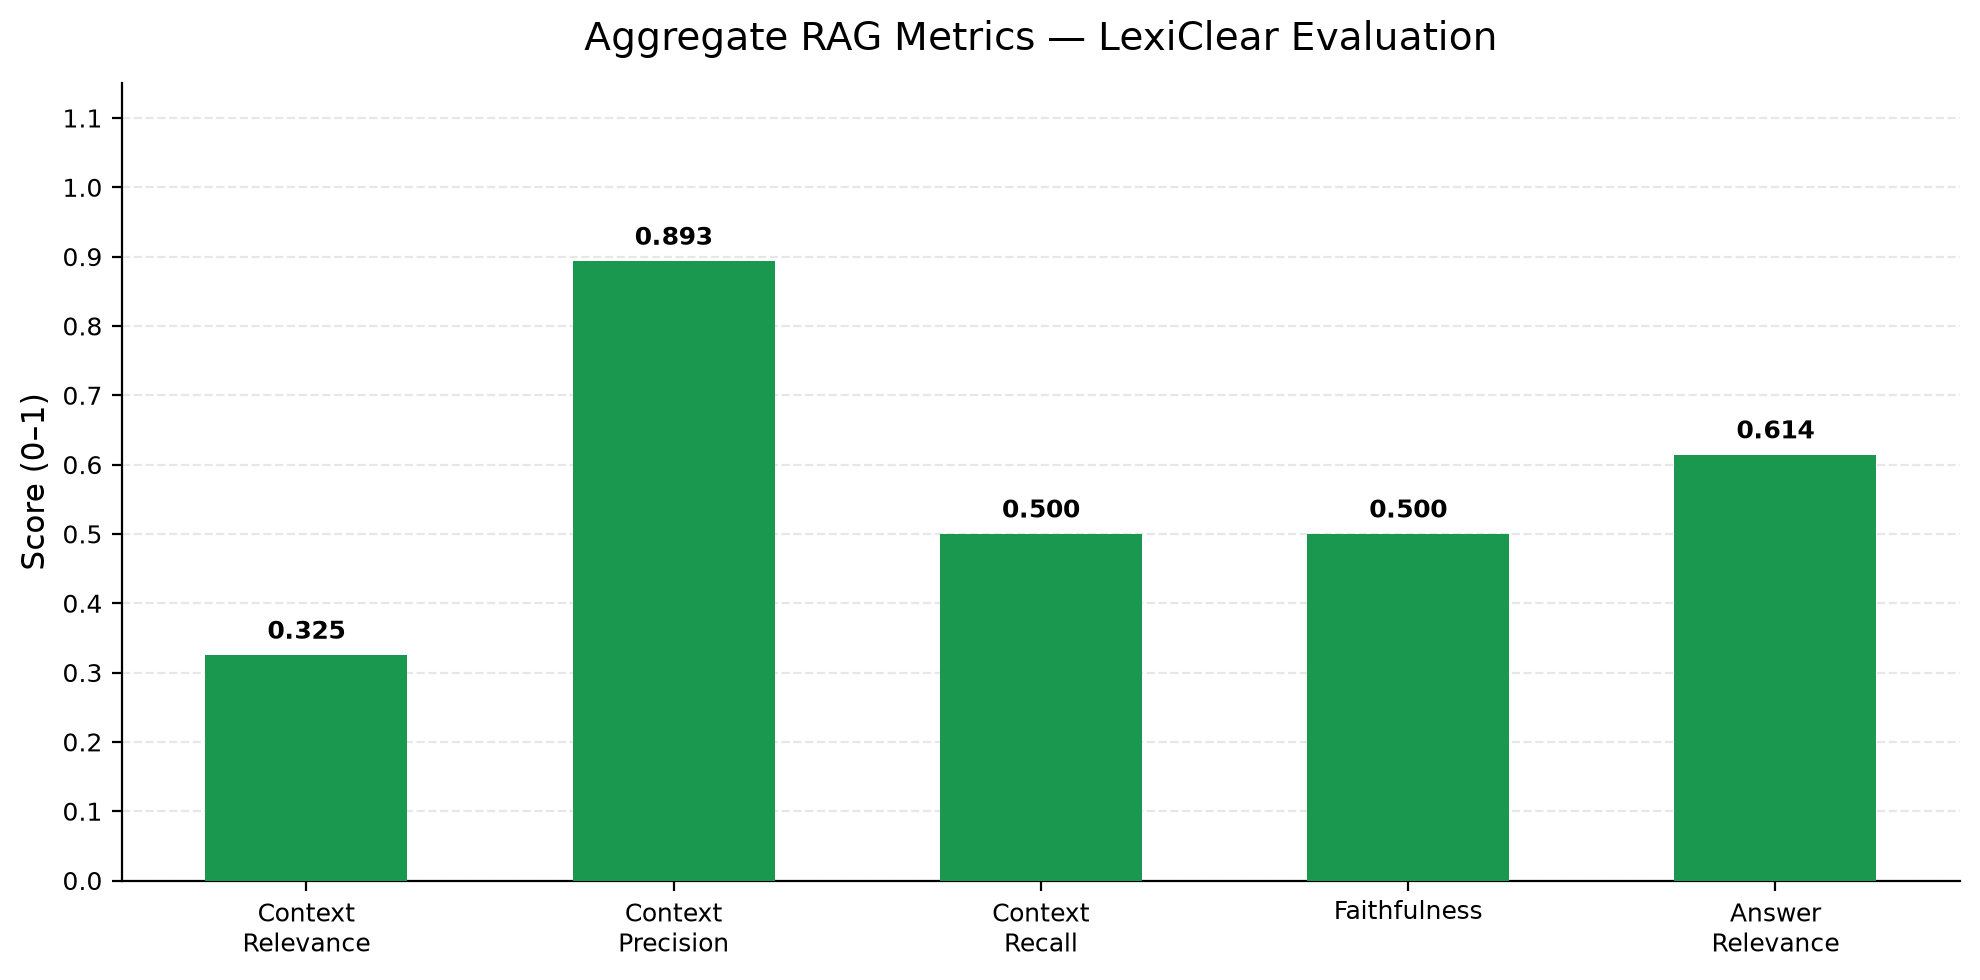
\includegraphics[width=0.90\textwidth]{aggregate_rag_metrics.png}
    \caption{Aggregate RAG Evaluation Metrics}
    \label{fig:aggregate_rag_metrics}
\end{figure}

Figure~\ref{fig:aggregate_rag_metrics} describes the aggregate RAG evaluation results across the 80 evaluated questions. Context Precision obtained a score of 0.986, whereas Context Relevance was 0.451. Context Recall and Faithfulness were both recorded as 0.500, while Answer Relevance was 0.759. These metrics provide separate measurements of retrieval quality, contextual coverage, generation grounding, and answer relevance.\newpage

\begin{figure}[htbp]
    \centering
    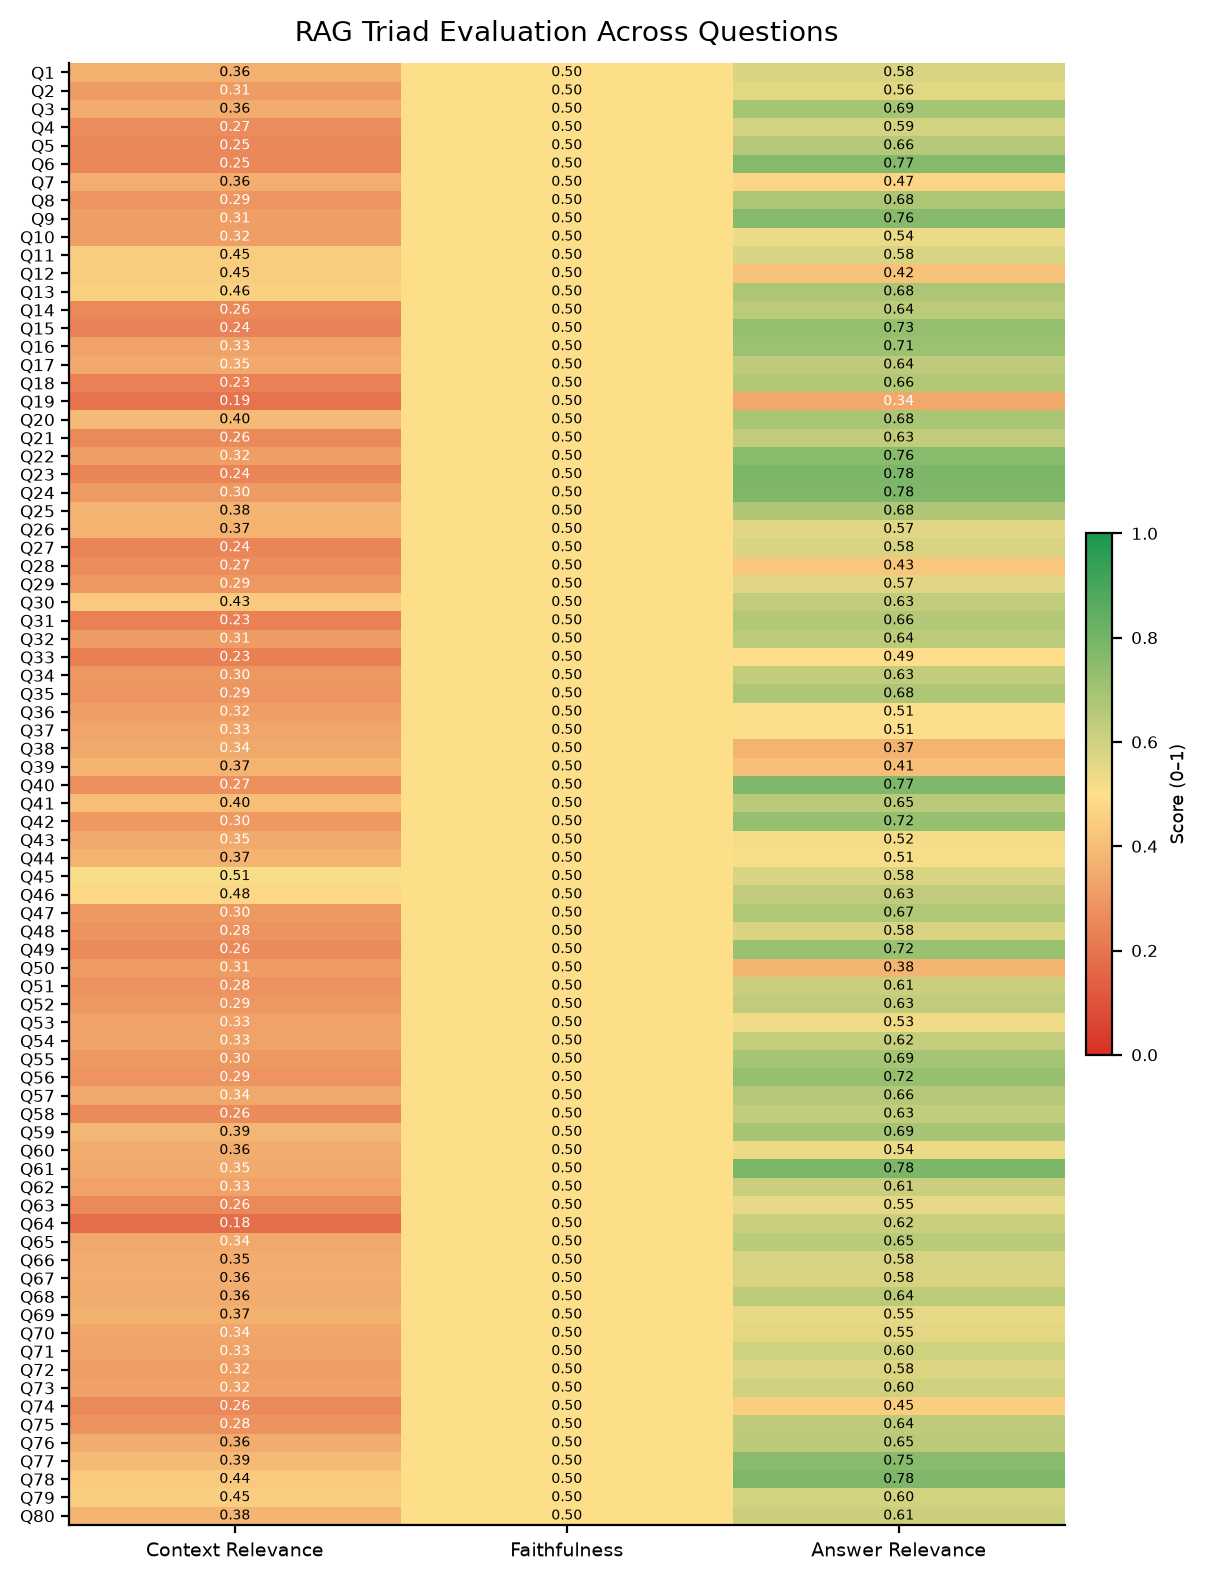
\includegraphics[width=0.62\textwidth]{rag_triad_heatmap.png}
    \caption{RAG Triad Evaluation Across the 80 Evaluated Questions}
    \label{fig:rag_triad_heatmap}
\end{figure}

Figure~\ref{fig:rag_triad_heatmap} presents the RAG Triad evaluation across the 80 question--answer pairs. The heatmap shows three dimensions of the RAG workflow: Context Relevance, Faithfulness and Answer Relevance. Context Relevance is how closely the retrieved document context matches the question that was asked. Faithfulness is how far the generated response stays grounded in that retrieved context, and Answer Relevance is how directly the response answers the question. The heatmap reports these metrics for each question and does not only give aggregate values.

The Context Relevance column varies across the evaluated questions, which tells us the retrieval component does not perform equally well for every query. Faithfulness values stay fairly steady across the questions, whereas Answer Relevance varies more. This makes it possible to pick out individual questions with lower retrieval or answer relevance for a closer look. The per-question view also helps show how retrieval quality relates to the quality of the final response. A question with low Context Relevance may mean that the retrieved chunks did not line up well with what the user asked for, leaving less useful evidence for the generation stage. However, comparatively stable Faithfulness values indicate that the responses generally remained connected to the retrieved context even when retrieval quality varied across individual questions. Differences in Answer Relevance can therefore be examined together with the corresponding Context Relevance values to understand whether reduced answer quality is associated with retrieval limitations. This question-level analysis provides a more detailed view of system behaviour than aggregate metrics alone.

\begin{figure}[htbp]
    \centering
    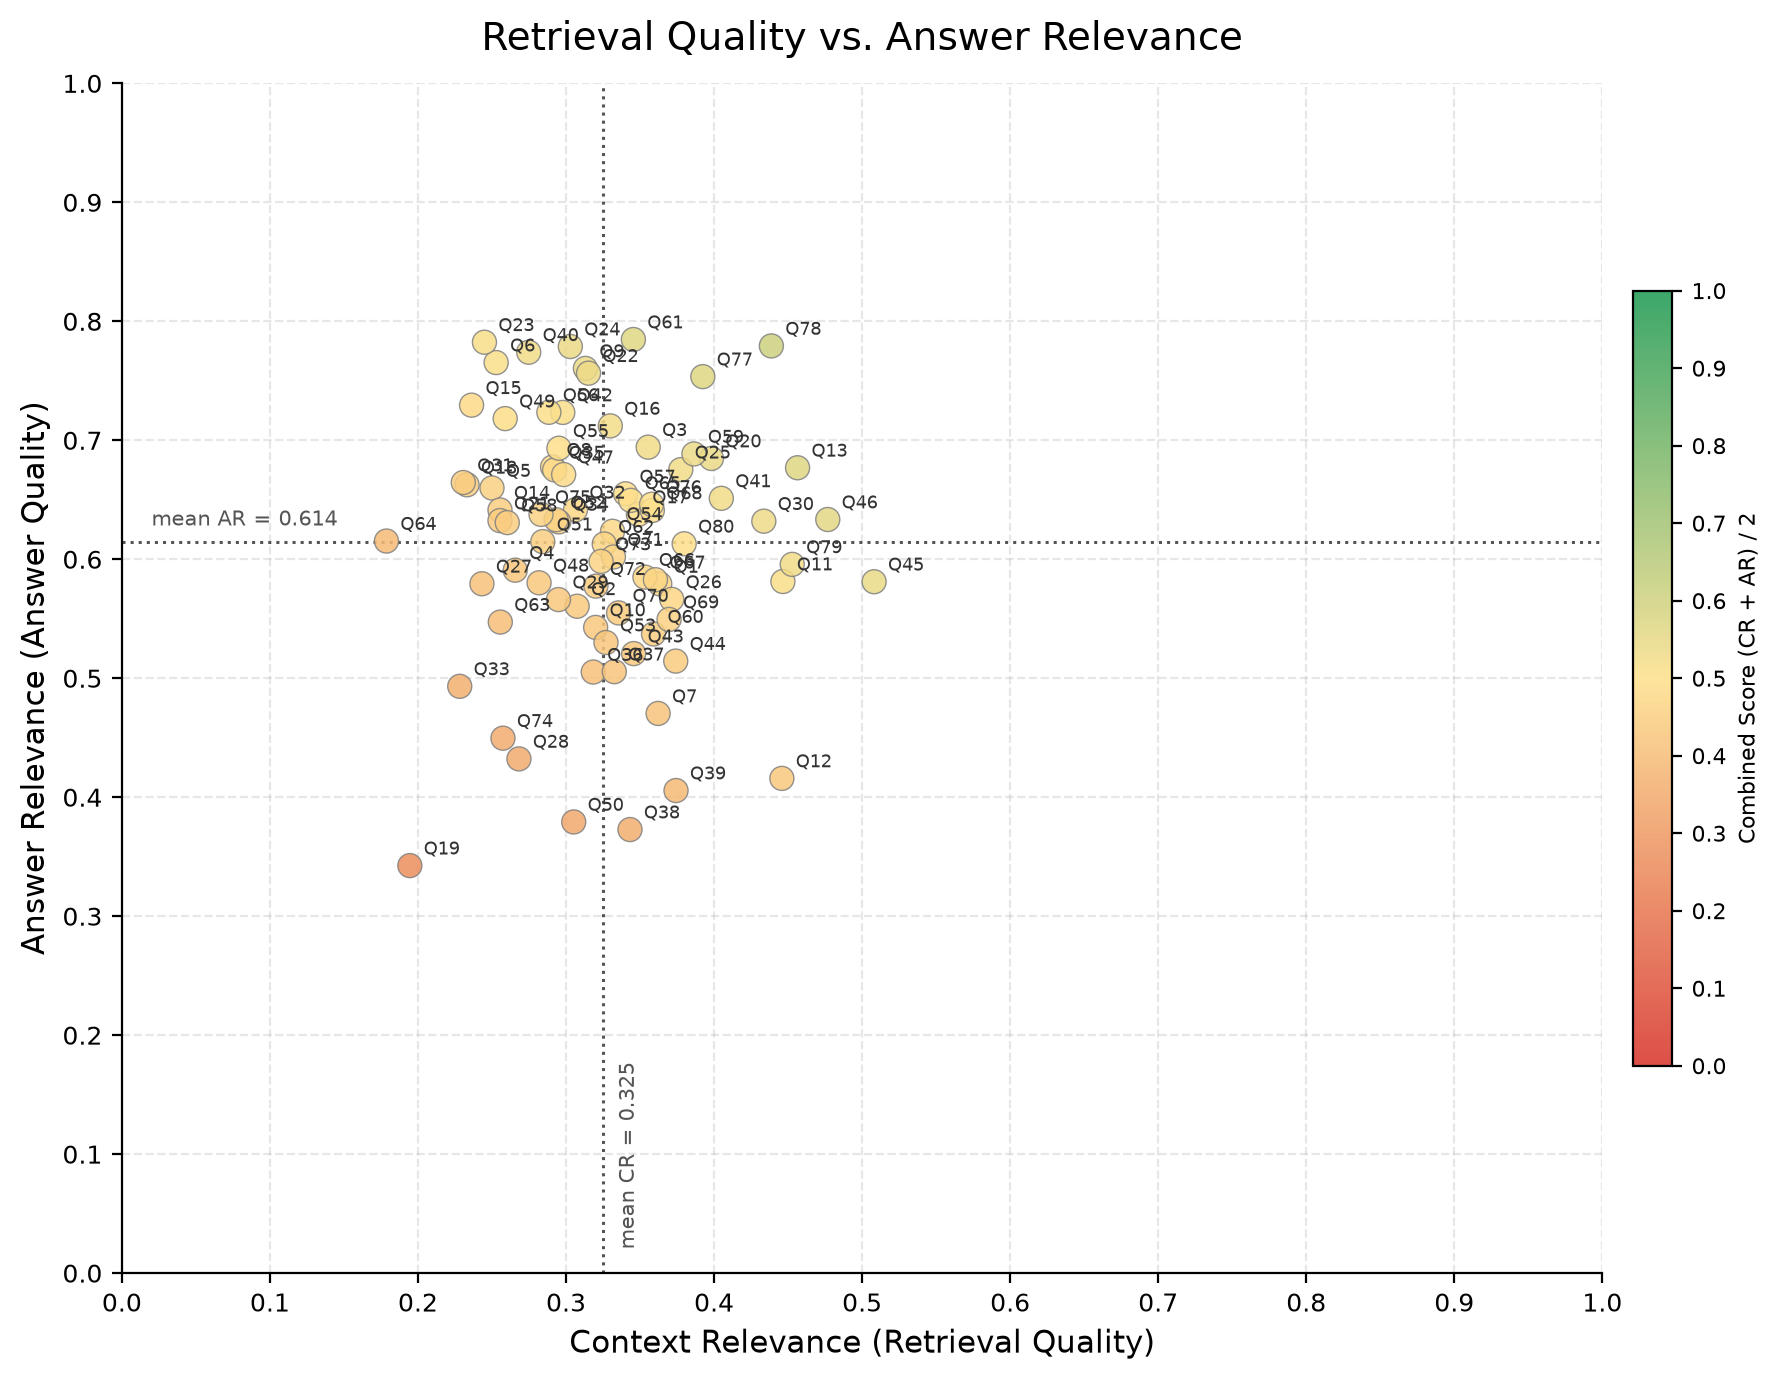
\includegraphics[width=0.78\textwidth]{retrieval_generation_quadrant.png}
    \caption{Relationship Between Context Relevance and Answer Relevance}
    \label{fig:retrieval_answer_scatter}
\end{figure}

Figure~\ref{fig:retrieval_answer_scatter} illustrates the relationship between retrieval quality and answer relevance for the evaluated questions. Context Relevance is represented on the horizontal axis, while Answer Relevance is represented on the vertical axis. Each point corresponds to one question in the evaluation set, allowing the distribution of individual question results to be examined.

The scatter distribution provides an additional way to examine whether differences in retrieved context are reflected in the relevance of the generated responses. Questions located in regions with higher Context Relevance indicate that the retrieval component identified context that was more closely related to the submitted query. The corresponding Answer Relevance values can then be examined to determine how the retrieved information was reflected in the generated response.

The distribution also illustrates why aggregate values alone are insufficient for interpreting the complete RAG behaviour. Two questions may contribute to the same average metric while exhibiting different combinations of retrieval and answer relevance. One question may obtain highly relevant context but produce a response with comparatively lower relevance, whereas another may receive moderately relevant context and still produce a response that closely addresses the question. Examining the individual points therefore provides a more detailed view of the relationship between retrieval and generation.

The per-question Context Relevance graph further supports this observation by showing the variation in retrieval behaviour across the complete evaluation set. The mean reference line gives a common point of comparison across the 80 questions. Questions that fall below it are cases where the retrieved context was less relevant to the query, so they are good candidates for investigating query formulation, chunking or retrieval configuration. The per-question Faithfulness graph likewise shows how consistently generated responses stayed linked to the retrieved context. That consistency matters for LexiClear because the system is supposed to explain information that is in the uploaded documents, and keeping the answer tied to retrieved evidence lowers the chance of a response drifting away from the source. Aggregate metrics and question-level charts give two complementary views of the RAG pipeline. The aggregates summarize how the evaluated system behaves overall, and the individual plots show variation that averaging would hide. That helps us choose specific cases to examine when we improve the retrieval and generation pipeline.

\begin{figure}[htbp]
    \centering
    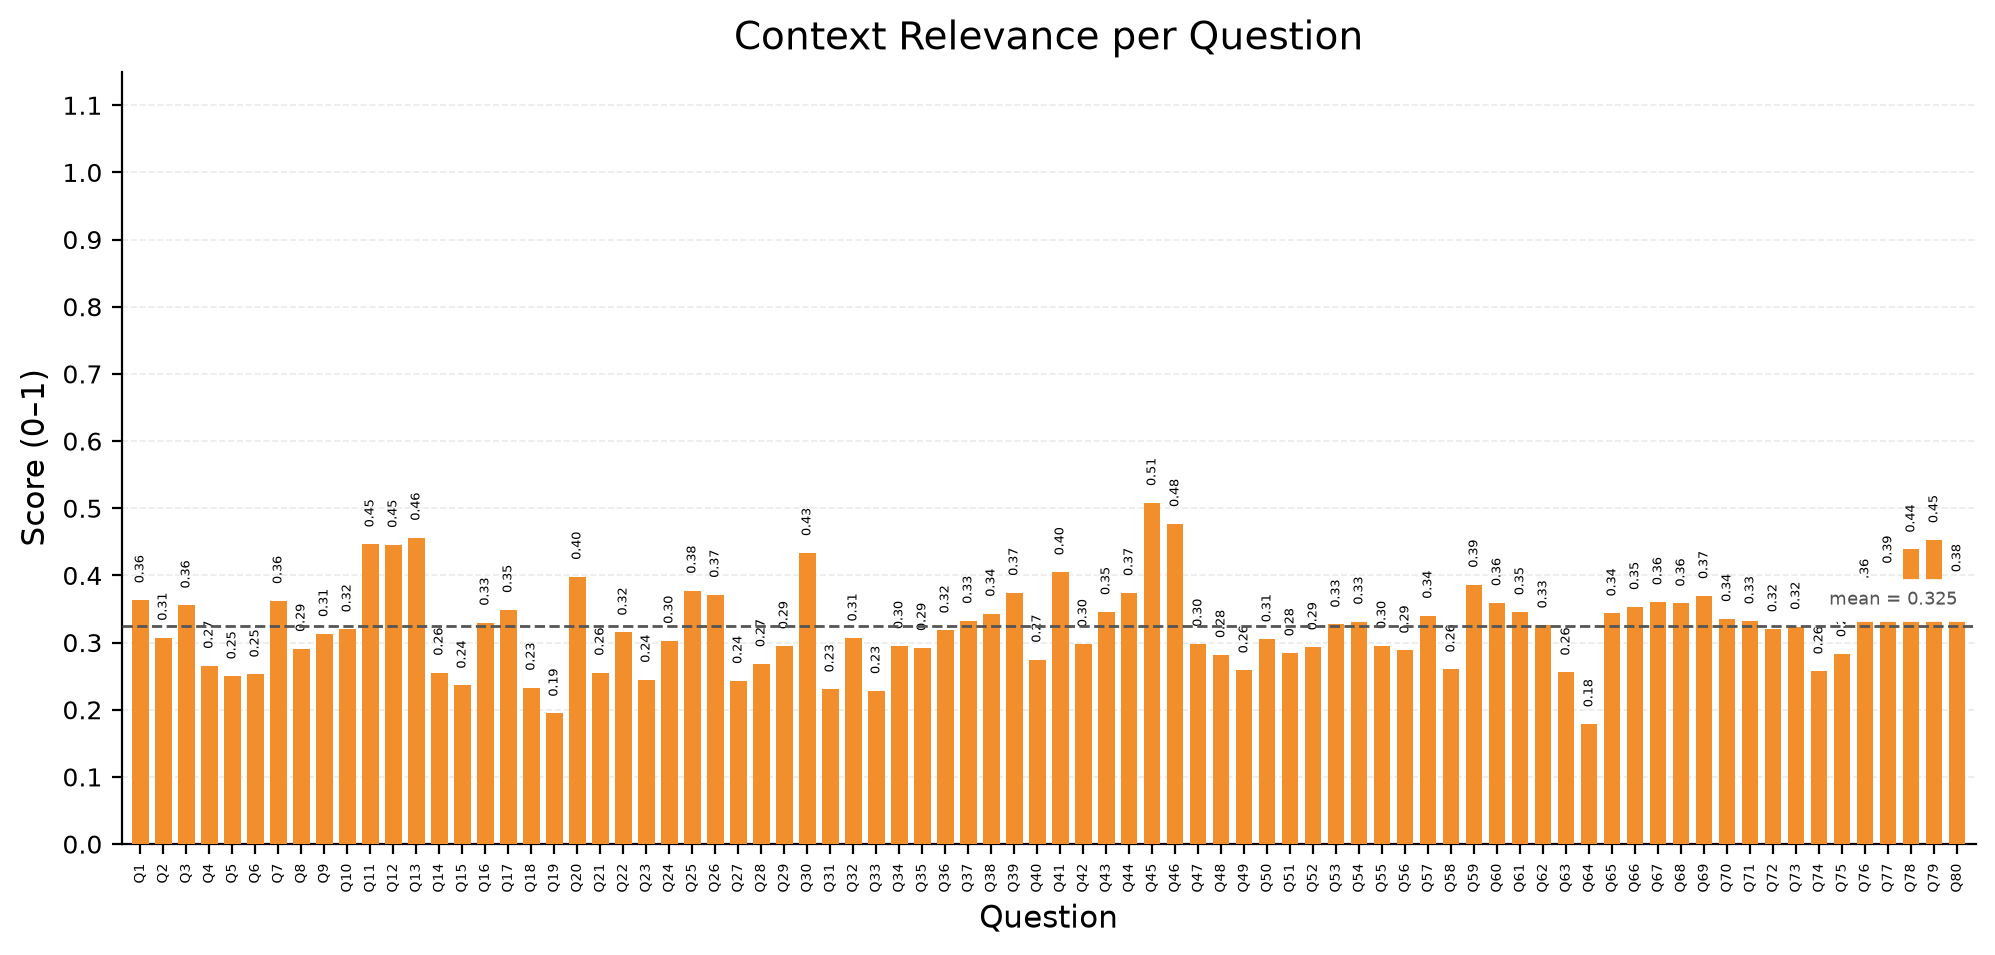
\includegraphics[width=0.92\textwidth]{question_context_relevance.png}
    \caption{Context Relevance Across the 80 Evaluated Questions}
    \label{fig:question_context_relevance}
\end{figure}

Figure~\ref{fig:question_context_relevance} shows the Context Relevance score for each of the 80 evaluated questions. The horizontal axis identifies the individual questions, while the vertical axis represents the Context Relevance score on a scale from 0 to 1. The dashed reference line represents the mean Context Relevance across the evaluation set.

The variation between questions indicates that retrieval quality depends on the individual query and the document content retrieved for that query. Questions with values above the mean received comparatively more relevant contextual information, whereas questions below the mean indicate cases where the retrieved context was less closely related to the query. This per-question analysis provides more detail than the aggregate Context Relevance value alone and helps identify queries that may require further retrieval or chunking improvements.

\begin{figure}[htbp]
    \centering
    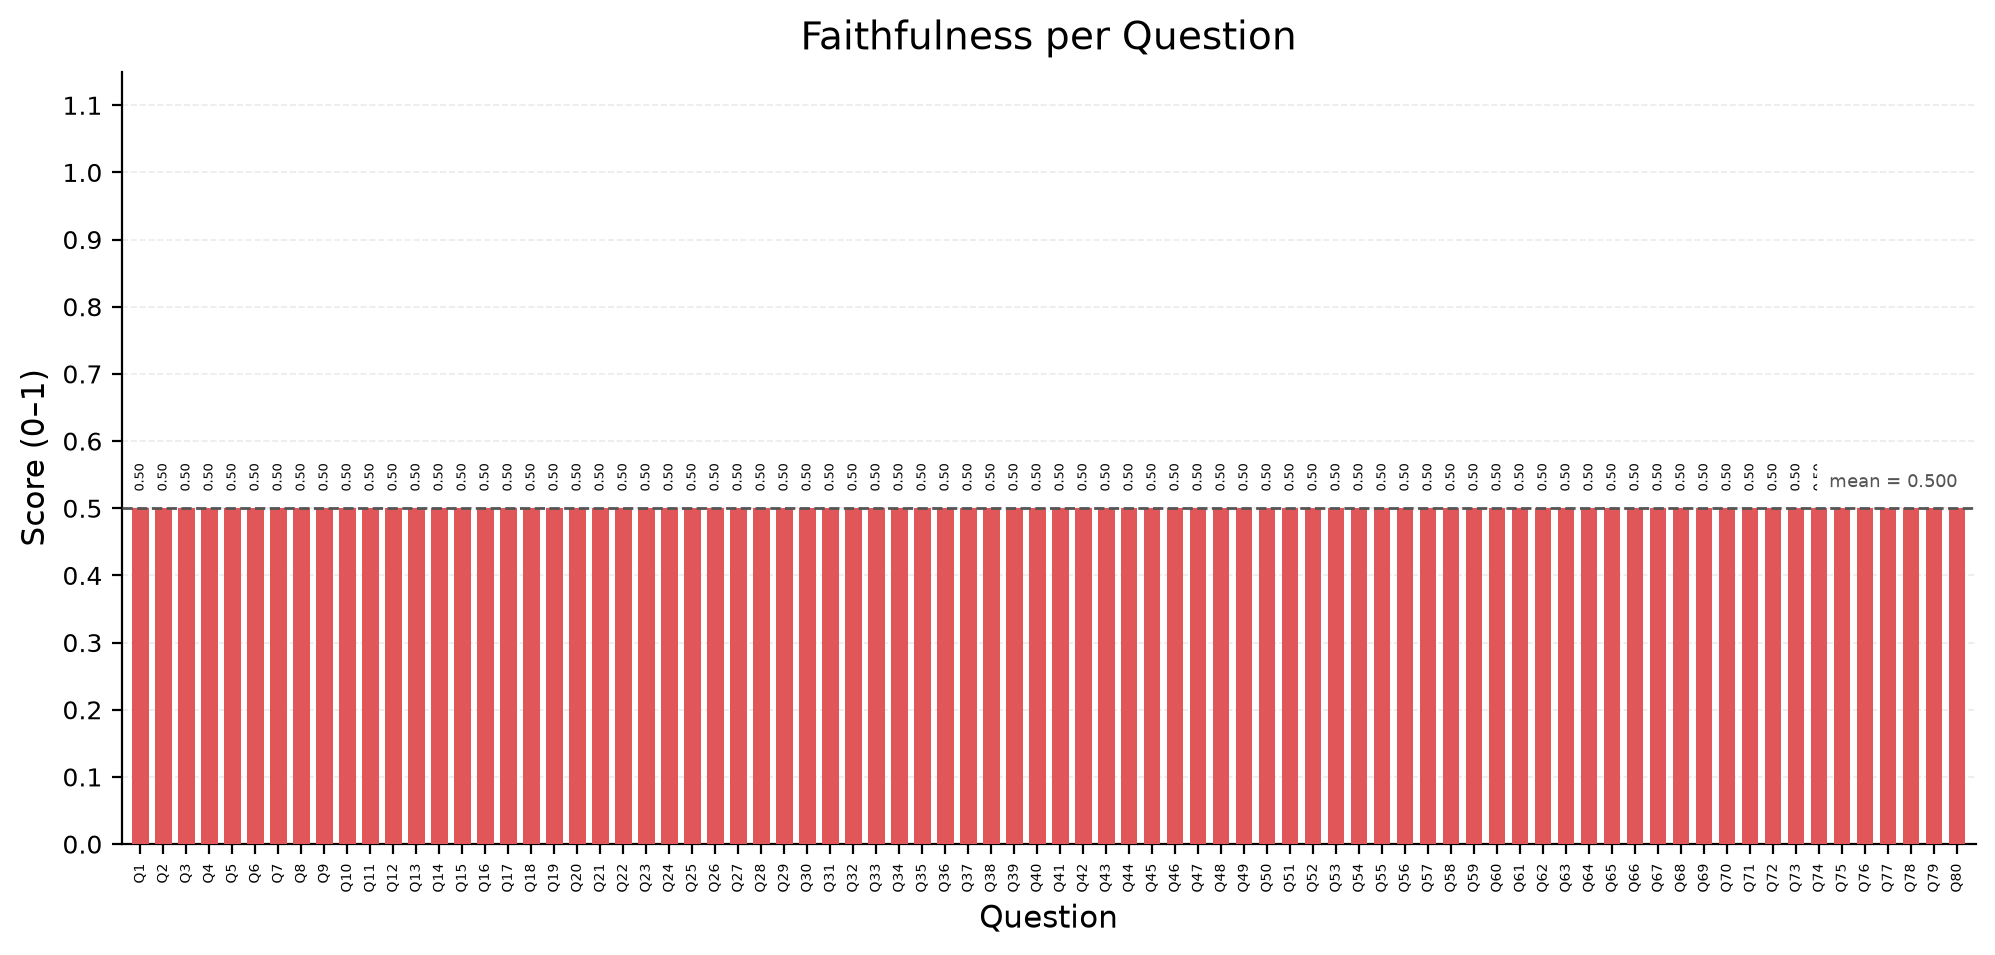
\includegraphics[width=0.92\textwidth]{question_faithfulness.png}
    \caption{Faithfulness Across the 80 Evaluated Questions}
    \label{fig:question_faithfulness}
\end{figure}

Figure~\ref{fig:question_faithfulness} presents the Faithfulness score for each evaluated question. Faithfulness measures how far the generated response agrees with the retrieved context given to the generation component. The dashed horizontal line marks the mean Faithfulness score over the evaluation set. Values stay fairly consistent across the questions, so the measurement was stable for the document and question set we evaluated. The graph also lets us spot individual questions that depart from the system's usual behaviour. A document-grounded legal information system has to keep its explanations tied to what the source document says, which is why this consistency matters.

Taken together, the RAG results suggest that a document-grounded system should not be judged on a single number. Retrieval decides what information reaches the generation component, while faithfulness and answer relevance show how that context is reflected in the final response. Looking at these dimensions separately lets us tell retrieval-related behaviour apart from generation-related behaviour. Question-level results are especially helpful because they show variation that aggregates cannot. A low Context Relevance value may mean the retrieved content did not match the question closely, and a lower Answer Relevance value may mean the response did not address the requested information directly. Observations like these point to individual queries for inspection, so we do not have to assume the whole evaluation set behaves the same way. The RAG evaluation also underlines how much source grounding matters across the whole processing pipeline.

Retrieval quality, contextual grounding and answer relevance all contribute to how useful the document question-answering workflow is. The measurements have to be read within the scope of the evaluation. The 80 questions are one particular set of document-related queries, and they do not cover every possible legal question, document structure or jurisdiction. The metrics also capture only certain aspects of retrieval and generation behaviour and are not a direct measure of legal correctness. What they do give is a basis for deciding where the system can be refined. Changes to chunking, semantic retrieval, query processing and context selection could be tested on the same question set in future experiments, and repeating the evaluation after each change would show systematically what effect it had on retrieval and generation. The purpose of retrieval is not simply to provide additional text to the language model, but to provide document-specific evidence that can support the generated response. 

\subsection{Question-Answer Evaluation Results}

The Ask LexiClear functionality was evaluated using 80 document-specific question-answer pairs. We compared the AI-generated answers with the expected answers using Semantic Similarity and BERTScore-based measures. Semantic Similarity measures how alike the generated and expected answers are, and BERTScore evaluates their semantic correspondence through Precision, Recall and F1. The evaluation also records QA Accuracy, based on the similarity threshold defined in the evaluation implementation. This question-answer evaluation is a direct assessment of what Ask LexiClear produces. The RAG metrics look separately at retrieval and grounding, but here the generated response is compared with an expected answer for each document-specific question. That gives another angle on whether what the system returns matches the intended answer in the evaluation set. Semantic Similarity shows how close the meaning of the generated response is to the expected answer, which is useful in document question answering because two answers can use different words and still say much the same thing. BERTScore adds a complementary comparison through Precision, Recall and F1, so answers can be compared along several dimensions and not only by exact text matching. The BERTScore values we obtained tell us more about the semantic relationship between generated and expected responses. In particular, the Recall value measures the extent to which information represented in the expected answer is reflected in the generated response, while Precision considers the correspondence of information produced by the system with the reference answer. The F1 measure combines these two aspects into a single value representing their balance.

The evaluation is especially relevant to LexiClear because legal questions may permit more than one valid formulation of an answer. A generated response does not necessarily need to reproduce the expected answer word-for-word to convey the same document-specific information. Semantic evaluation metrics are therefore more appropriate for this type of assessment than simple textual matching alone. The results should nevertheless be interpreted with consideration of the construction of the expected answers. The evaluation compares generated responses against the predefined answers contained in the test set, meaning that the measurements reflect similarity to those references. A response that differs semantically from the reference may receive a lower score even when more evaluation would be needed to say whether it is legally or contextually acceptable. A high similarity score, equally, does not by itself establish that a response is legally correct. The per-question Answer Relevance graph adds to the aggregate answer-quality measurements by showing how relevance varies from question to question, so we can see where the generated response lines up closely with the requested information and where the alignment is weaker. That kind of question-level analysis points to cases worth examining when the system is refined. The Semantic Similarity score we obtained was 0.8108. BERTScore Precision, Recall and F1 were 0.8957, 0.9393 and 0.9167 respectively, and the recorded QA Accuracy was 0.7625.

\begin{figure}[htbp]
    \centering
    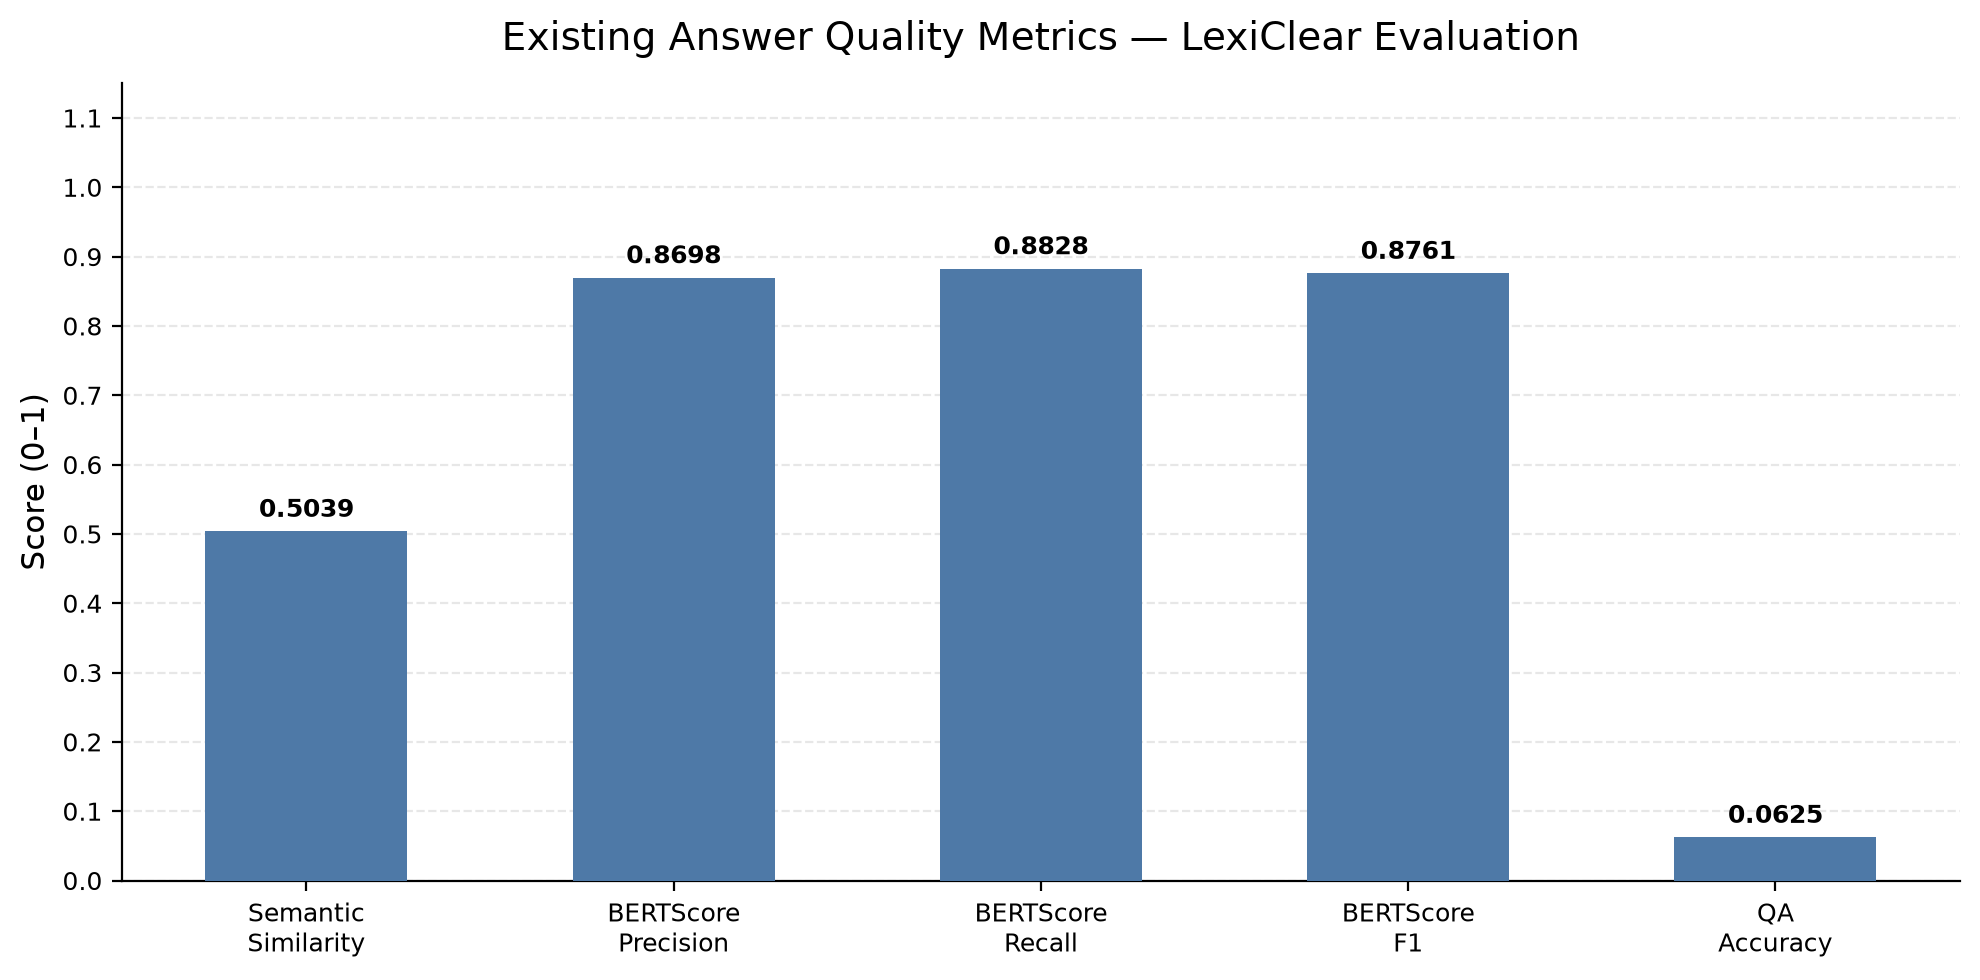
\includegraphics[width=0.90\textwidth]{answer_quality_metrics.png}
    \caption{Answer Quality Evaluation Metrics}
    \label{fig:answer_quality_metrics}
\end{figure}

Figure~\ref{fig:answer_quality_metrics} describes the answer-quality evaluation results obtained from the 80 question-answer pairs. The Semantic Similarity score of 0.8108 indicates the measured similarity between the generated and expected answers. The BERTScore Precision, Recall, and F1 values of 0.8957, 0.9393, and 0.9167 respectively provide additional measures of semantic correspondence between the generated and reference answers. The QA Accuracy of 0.7625 represents the proportion of evaluated questions that satisfied the similarity threshold used by the evaluation procedure. These results provide a quantitative assessment of the generated responses for the tested question set. The metrics are reported within the scope of the 80 document-specific questions used for the evaluation and should not be interpreted as a general measure of legal accuracy.

\begin{table}[htbp]
\centering
\caption{Aggregate Question-Answer Evaluation Metrics}
\label{tab:qa_metrics}

\vspace{0.15cm}

\renewcommand{\arraystretch}{1.5}

\begin{tabular}{|p{8cm}|p{4cm}|}
\hline
\textbf{Evaluation Metric} & \textbf{Value} \\
\hline
Questions Evaluated & 80 \\
\hline
Average Semantic Similarity & 0.8108 \\
\hline
Average BERTScore Precision & 0.8957 \\
\hline
Average BERTScore Recall & 0.9393 \\
\hline
Average BERTScore F1 & 0.9167 \\
\hline
QA Accuracy & 0.7625 \\
\hline
\end{tabular}
\end{table}

Table~\ref{tab:qa_metrics} shows evaluation which was performed on 80 question-answer pairs. The average Semantic Similarity score was 0.8108, while the average BERTScore Precision, Recall, and F1 values were 0.8957, 0.9393, and 0.9167, respectively. The recorded QA Accuracy was 0.7625.

\begin{figure}[htbp]
    \centering
    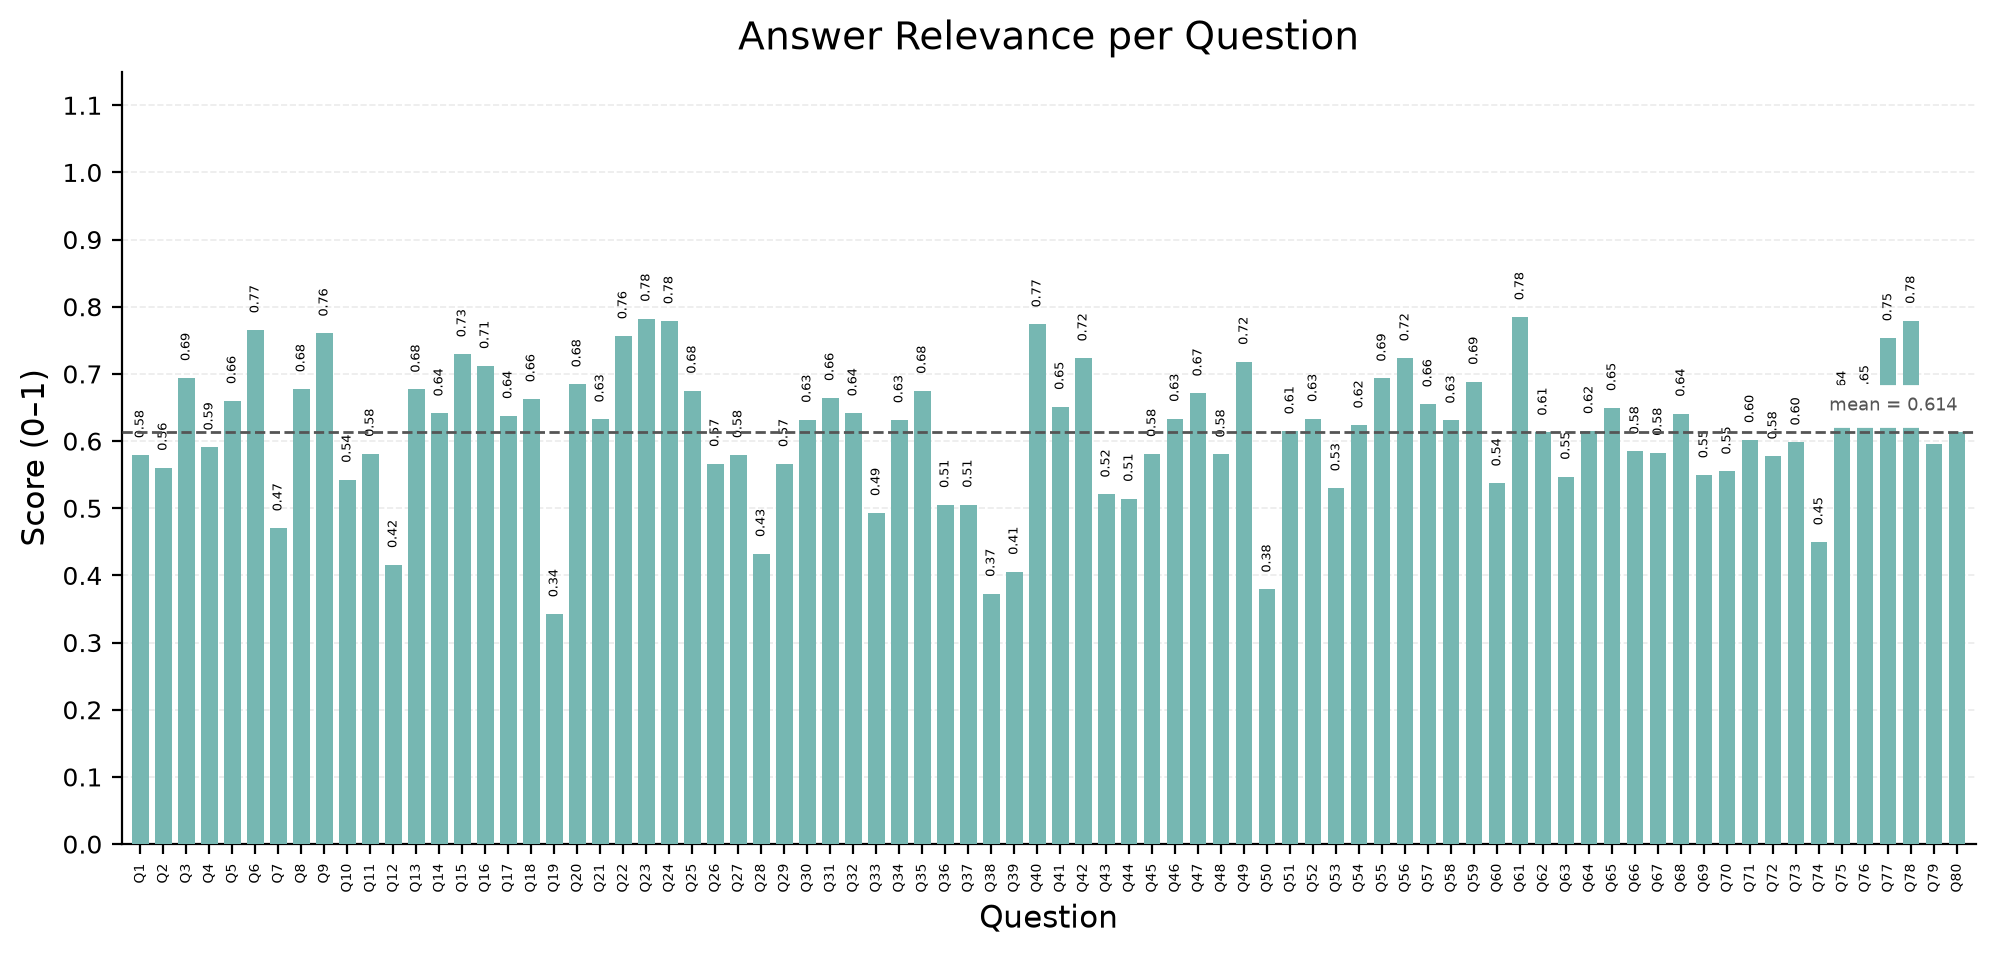
\includegraphics[width=0.92\textwidth]{question_answer_relevance.png}
    \caption{Answer Relevance Across the 80 Evaluated Questions}
    \label{fig:question_answer_relevance}
\end{figure}

Figure~\ref{fig:question_answer_relevance} presents the Answer Relevance score for each of the 80 evaluated questions. The score measures how directly the generated response addresses the corresponding user question. The dashed horizontal line represents the mean Answer Relevance across the evaluation set.

The variation across the questions shows that the generated responses do not have identical levels of relevance for every query. Higher scores mean the response is more closely aligned with the information requested, and lower scores mean weaker alignment. The per-question graph adds to the aggregate evaluation by showing how answer relevance is distributed across the whole question set.

Comparing the aggregate answer-quality measures with the per-question Answer Relevance results also tells us about the consistency of the question-answering component. The aggregates summarize the overall behaviour on the 80 evaluated questions, while individual results show that response quality can change with the information being asked for. We expected this in document-based question answering, since different questions need different parts of the source and differ in how specific they are. A question about information that is clearly stated in the document is a different case from one that needs information combined across several clauses or sections. The second kind asks more of both retrieval and generation, because the required information must first be found and then worked into a coherent response.

The evaluation also shows the value of using several metrics together. Semantic Similarity gives a general measure of how well generated and expected answers correspond, BERTScore adds separate Precision, Recall and F1 figures, and Answer Relevance considers how directly a response addresses the question. Combined, they describe the behaviour of the generated answers more fully than any one metric could. The results can also be read alongside the earlier RAG evaluation. Retrieval metrics describe the quality and coverage of the context given to the generation component, whereas the question-answer evaluation checks the resulting response against the expected answer. Differences in answer quality can therefore be looked at together with the retrieval and faithfulness results, to see whether particular questions point to weaker retrieval or weaker generation.

Although this evaluation is quantitative, it does not take the place of human or expert assessment of legal information. Semantic comparison tells us whether generated answers match the predefined references. It cannot tell us whether an answer is legally valid, complete or appropriate for a real situation, so expert evaluation would be an important extension in future versions. Overall, the results show that Ask LexiClear can be evaluated systematically with predefined document-specific questions and multiple semantic metrics. They give measurable evidence about how responses behave while keeping automated answer similarity separate from authoritative legal correctness, a distinction that matters a great deal for a system meant to help people understand legal and administrative documents. These results provide a quantitative assessment of the responses generated by the Ask LexiClear functionality for the tested questions. The Semantic Similarity and BERTScore measures indicate the degree of similarity between the generated and expected answers, while the QA Accuracy represents the proportion of evaluated questions satisfying the similarity threshold used by the evaluation procedure. The evaluation was conducted on a document-specific set of 80 questions and therefore represents the measured performance for the tested question set. The reported values should not be interpreted as a general measure of legal accuracy or legal interpretation capability.





\subsection{Jurisdiction Grounding Results}
The jurisdiction grounding component was integrated into the response-generation workflow. The selected jurisdictional context can be passed along with the retrieved document information before the response is generated, giving an extra layer of context for explanations where legal or administrative information varies by jurisdiction. It guides the response and is not a replacement for the source document. How well it works depends on the configured jurisdictional information and the supporting sources available. What our functional result shows is that the feature is integrated into the system. It is not a quantitative evaluation of jurisdiction-specific legal accuracy.

\subsection{Multilingual Output Results}
LexiClear gives output in English, Hindi and Kannada, and the generated response can be processed according to the language the user picks. This takes the system past English-only interaction and lets information from formal documents reach people in languages they know. Translation works on the generated response, and the original document stays the primary source of anything document-specific. We did not run a controlled translation benchmark or an expert linguistic evaluation during the testing available, so the results establish functional multilingual support and do not claim a numerical translation-quality score.

\subsection{Text-to-Speech Results}
The text-to-speech component was tested as part of the accessibility workflow. During development testing, the system successfully generated a WAV audio file for Kannada text using the available Apple MPS device configuration. The frontend also provides Listen and Stop controls for interacting with the generated audio. This establishes a connection between the generated textual response and the speech-output interface. The speech functionality provides an alternative method of accessing generated information, particularly for users who may prefer listening to the explanation rather than reading the complete response. Further evaluation across all supported languages and different types of legal terminology would be required for a comprehensive assessment of speech quality.
\subsection{Overall Discussion}
The functional testing demonstrates that the major components of LexiClear have been connected into an end-to-end workflow. d systematic evaluation of retrieval, generation, translation and speech quality have not yet been completed. What we present here are functional and integration results and not statistical performance results. Future evaluation can strengthen the assessment with expert-annotated legal documents, predefined test questions, source-grounding measurements, multilingual evaluation and user-based usability studies.

\chapter{Software Testing}

\section{Introduction}
Testing is how we find out whether LexiClear actually does what we said it would, and just as usefully, where it does not yet. This chapter sets out a module-wise functional test suite of 42 test cases spread over ten modules: document upload, document analysis, key clause extraction, rights and obligations extraction, risk analysis, jurisdictional context, Ask LexiClear (RAG), multilingual support, text-to-speech, and system performance and error handling.

Every test case has an ID, a scenario, an expected result, an actual result and a status. The scenarios come straight from the features described in the earlier chapters, and we did not invent extra functionality just to have something to test. Where Chapter~4 already reports what we observed, the Actual Result column points to that section. Where Chapter~4 gives measured retrieval or question-answering values, we have copied them over as recorded.

\textbf{A note on the status of these results.} The Pass and Fail entries in this chapter are provisional. They were drafted for review and are not yet backed by a recorded test run. Any entry marked ``to be confirmed'' has to be checked against an actual execution before it is quoted as a verified result, and we do not claim otherwise here.

\textbf{Where the tests are reported.} All test cases for the project appear in this chapter only. Chapter~4 covers the experimental results and the overall discussion (Section~4.3). For functionality where Chapter~4 records no observation, such as OCR processing, invalid-file handling, Hindi output and the Listen and Stop controls, the entry here is a provisional draft waiting for validation.

\section{Functional Testing}
In functional testing we take each module in turn and compare what it does with what it should do. The test cases are listed in Tables~5.1 to~5.10. In every table, Pass and Fail are provisional statuses until they are validated.

We wrote the test cases to do more than confirm that things work. Most of them are ordinary checks, such as uploading a clean PDF, asking a question about it or picking a language. We also included cases that try to break the system on purpose: a corrupted file, a question asked before any document has been processed, and a contract with no risk clauses at all. A third group probes the weak spots we already knew about, like low-quality scans, long documents and legal terminology in translation. Those cases are the most likely to fail, and they are the ones that tell us the most.

The Actual Result column comes from three places. Where we saw something happen during development on a macOS machine, with the React frontend talking to the FastAPI backend, we say so and point to the section of Chapter~4 that describes it. Where Chapter~4 gives a measured number from the 80-question evaluation, we copy that number over as it was recorded. For everything else, the entry is a provisional draft marked ``to be confirmed''. Read the tables with that in mind. A Pass next to a Chapter~4 reference is on firmer ground than a Pass that still waits for someone to run the test.

\needspace{18\baselineskip}
\subsection{Document Upload Module}
Table~\ref{tab:upload} lists the four test cases for this module (TC01 to TC04). Provisionally, three passed and one failed.
{\footnotesize
\setlength{\tabcolsep}{3pt}
\renewcommand{\arraystretch}{1.15}
\begin{longtable}{|p{0.075\linewidth}|p{0.19\linewidth}|p{0.23\linewidth}|p{0.32\linewidth}|p{0.08\linewidth}|}
\caption{Test Cases for Document Upload Module}\label{tab:upload}\\
\hline
\textbf{Case ID} & \textbf{Test Scenario} & \textbf{Expected Result} & \textbf{Actual Result} & \textbf{Status}\\
\hline
\endfirsthead
\multicolumn{5}{c}{\tablename~\thetable{} (continued)}\\
\hline
\textbf{Case ID} & \textbf{Test Scenario} & \textbf{Expected Result} & \textbf{Actual Result} & \textbf{Status}\\
\hline
\endhead
\hline
\multicolumn{5}{r}{\emph{Continued on next page}}\\
\endfoot
\hline
\endlastfoot
TC01 & Upload a valid digital legal PDF (a rental agreement) through the frontend & The interface accepts the document and passes it to the backend for processing & The document was accepted through the upload interface and handed to the backend (Section~4.3.1) & Pass\\
\hline
TC02 & Upload a scanned or image-based PDF that needs OCR & Text is obtained through OCR and the document enters the normal processing workflow & OCR text was obtained and the document moved into the workflow. To be confirmed against an execution record & Pass\\
\hline
TC03 & Upload an unsupported file type or a corrupted PDF & Validation stops the file before extraction or OCR (Section~3.2.1) and the interface says it cannot be processed & The file was not passed on and a message was shown. To be confirmed, and the exact message still needs to be recorded & Pass\\
\hline
TC04 & Upload a low-quality scanned PDF & OCR returns text complete enough for reliable preprocessing, chunking and retrieval & The extracted text was incomplete for the low-quality scan, which fits the OCR limitation in Section~6.1. To be confirmed & Fail\\
\end{longtable}
}

TC01 and TC02 check that both a digital PDF and a scanned one get through the front door, the second relying on OCR. TC03 checks that the validation stage from Section~3.2.1 keeps an unsupported or corrupted file away from extraction. TC04 looks at the quality of text coming out of a poor scan, and its provisional failure is no surprise: OCR errors travel downstream and can affect preprocessing, chunking, retrieval and the final response. Every later module depends on this one, which is why upload validation and OCR quality matter more than they might first appear. A system that cannot tell a clean PDF from an unreadable scan will give shaky answers however good its retrieval is.

\needspace{18\baselineskip}
\subsection{Document Analysis Module}
Table~\ref{tab:analysis} lists the four test cases for this module (TC05 to TC08). Provisionally, three passed and one failed.
{\footnotesize
\setlength{\tabcolsep}{3pt}
\renewcommand{\arraystretch}{1.15}
\begin{longtable}{|p{0.075\linewidth}|p{0.19\linewidth}|p{0.23\linewidth}|p{0.32\linewidth}|p{0.08\linewidth}|}
\caption{Test Cases for Document Analysis Module}\label{tab:analysis}\\
\hline
\textbf{Case ID} & \textbf{Test Scenario} & \textbf{Expected Result} & \textbf{Actual Result} & \textbf{Status}\\
\hline
\endfirsthead
\multicolumn{5}{c}{\tablename~\thetable{} (continued)}\\
\hline
\textbf{Case ID} & \textbf{Test Scenario} & \textbf{Expected Result} & \textbf{Actual Result} & \textbf{Status}\\
\hline
\endhead
\hline
\multicolumn{5}{r}{\emph{Continued on next page}}\\
\endfoot
\hline
\endlastfoot
TC05 & Request structured analysis of the processed rental agreement through the backend analysis endpoint & Output is organised into summary, key clauses, risks, obligations, rights and required actions, where applicable & The endpoint returned structured information for the document (Section~4.3.2) & Pass\\
\hline
TC06 & Generate the document summary & A summary of the document's purpose and main content, grounded in the uploaded file & A document-grounded summary was displayed. To be confirmed against an execution record & Pass\\
\hline
TC07 & Generate the required actions section & Actions the user must complete are listed wherever the document specifies them & Required actions were listed for the tested document. To be confirmed against an execution record & Pass\\
\hline
TC08 & Analyse a lengthy document with many clauses & Every analysis category is filled in and agrees with the document & Coverage of the categories was uneven for the long document, and category correctness was not checked by experts (Section~4.3.2). To be confirmed & Fail\\
\end{longtable}
}

TC05 confirms that the output comes back sorted into its categories, and TC06 and TC07 look at the summary and the required actions on their own. TC08 asks the harder question of whether every category is populated when the document is long and clause-heavy. It failed provisionally because coverage was uneven and because nobody with legal expertise has reviewed whether the categories are correct, so the analysis still has to be read against the original document (Section~6.1).

It is worth being clear about what these four cases do and do not show. They show that each output category exists and that the analysis behaves on a longer document. They do not show that the content is legally right. Making the analysis dependable across documents of different lengths is the main thing this module still needs. In the above Test Cases we can see that there ahs been 3 pass cases for TC05, TC06 and TC07. Then only for TC08 we have one failed case.

\needspace{18\baselineskip}
\subsection{Key Clause Extraction Module}
Table~\ref{tab:clause} lists the three test cases for this module (TC09 to TC11). Provisionally, two passed and one failed.
{\footnotesize
\setlength{\tabcolsep}{3pt}
\renewcommand{\arraystretch}{1.15}
\begin{longtable}{|p{0.075\linewidth}|p{0.19\linewidth}|p{0.23\linewidth}|p{0.32\linewidth}|p{0.08\linewidth}|}
\caption{Test Cases for Key Clause Extraction Module}\label{tab:clause}\\
\hline
\textbf{Case ID} & \textbf{Test Scenario} & \textbf{Expected Result} & \textbf{Actual Result} & \textbf{Status}\\
\hline
\endfirsthead
\multicolumn{5}{c}{\tablename~\thetable{} (continued)}\\
\hline
\textbf{Case ID} & \textbf{Test Scenario} & \textbf{Expected Result} & \textbf{Actual Result} & \textbf{Status}\\
\hline
\endhead
\hline
\multicolumn{5}{r}{\emph{Continued on next page}}\\
\endfoot
\hline
\endlastfoot
TC09 & Identify key clauses in the rental agreement, such as duration, payment and termination & The key clauses are found and shown in the key clauses section & Key clauses were identified and displayed. To be confirmed against an execution record & Pass\\
\hline
TC10 & Present an identified clause in simplified language & The clause is explained so that a non-specialist can follow it, without losing its meaning & Clauses were presented in simplified wording. To be confirmed against an execution record & Pass\\
\hline
TC11 & Trace an extracted clause back to its source clause or section & The user is shown which clause or section supports each extracted clause & No source reference was shown alongside the extracted clause. Source and clause-level traceability is listed as future work (Section~6.2) & Fail\\
\end{longtable}
}

These three cases separate what is found, how it is explained, and whether it can be checked. TC09 looks at whether the important clauses, such as duration, payment and termination, are picked out. TC10 looks at whether they are explained in plain language without changing their meaning. TC11 asks whether the user can see where in the document a clause came from, and it is the one that fails: traceability is not built yet, and Section~6.2 lists it as future work. With one failure out of three, the provisional pass rate for the module is 66.67\%.

Pulling out clauses is only half the job. People also need to understand them and be able to verify them, and the second part is missing for now. Until each clause points back to its source, the user has to search the original document themselves to confirm what the system says. These cases are not meant to judge legal correctness. They check that the clause section exists and reads clearly, and they show where the next piece of work lies.

Clause extraction is also where the quality of earlier stages becomes visible. A clause can only be picked out if the text around it was extracted cleanly and kept together when the document was chunked. When a clause such as the termination condition is split across two chunks, or contains a stray OCR error, the explanation shown to the user can end up incomplete even though the clause itself was found. For this reason we read TC09 and TC10 as tests of the whole pipeline up to that point, not just of the clause section on its own.

TC10 deserves one more comment. Simplifying a clause always risks changing what it says, and in a legal document a small change in wording, such as replacing ``shall'' with ``may'', alters the obligation. The aim of the simplified version is to help the reader understand the original, not to stand in for it. That is also why TC11 matters more than its single failure suggests: once each clause points to its source, a user can compare the plain-language version with the original wording and decide for themselves whether the simplification is fair.

\needspace{18\baselineskip}
\subsection{Rights and Obligations Extraction Module}
Table~\ref{tab:rights} lists the four test cases for this module (TC12 to TC15). Provisionally, three passed and one failed.
{\footnotesize
\setlength{\tabcolsep}{3pt}
\renewcommand{\arraystretch}{1.15}
\begin{longtable}{|p{0.075\linewidth}|p{0.19\linewidth}|p{0.23\linewidth}|p{0.32\linewidth}|p{0.08\linewidth}|}
\caption{Test Cases for Rights and Obligations Extraction Module}\label{tab:rights}\\
\hline
\textbf{Case ID} & \textbf{Test Scenario} & \textbf{Expected Result} & \textbf{Actual Result} & \textbf{Status}\\
\hline
\endfirsthead
\multicolumn{5}{c}{\tablename~\thetable{} (continued)}\\
\hline
\textbf{Case ID} & \textbf{Test Scenario} & \textbf{Expected Result} & \textbf{Actual Result} & \textbf{Status}\\
\hline
\endhead
\hline
\multicolumn{5}{r}{\emph{Continued on next page}}\\
\endfoot
\hline
\endlastfoot
TC12 & Extract the rights available to each party & The rights are listed in the rights section & Rights were listed for the tested document. To be confirmed against an execution record & Pass\\
\hline
TC13 & Extract the obligations of each party & The obligations are listed in the obligations section & Obligations were listed for the tested document. To be confirmed against an execution record & Pass\\
\hline
TC14 & Separate the responsibilities of different parties, such as landlord and tenant & Rights and obligations are assigned to the correct party & Responsibilities were assigned to the parties in the tested document. To be confirmed against an execution record & Pass\\
\hline
TC15 & Extract obligations that carry exceptions or cross-references & Conditions, exceptions and cross-referenced provisions are captured along with the obligation & The conditional parts of some obligations were not captured. To be confirmed & Fail\\
\end{longtable}
}

TC12 and TC13 check that rights and obligations are listed at all, and TC14 checks that they land with the right party, for instance the landlord or the tenant in a rental agreement. TC15 is the difficult one. Obligations often come with exceptions or point to other clauses, and the condition has to travel with the obligation for the summary to be honest. In our draft run some of those conditional parts were lost, so the obligations list should be read together with the original clauses.

These cases only deal with what the document states. Whether a right or obligation could actually be enforced is a legal question the functional tests do not touch. With one failure in four, the provisional pass rate here is 75.00\%, as Table~\ref{tab:test-summary} shows.

A rental agreement shows why TC14 and TC15 are worth testing. The same document puts duties on the landlord and the tenant, and a single sentence can switch between the two. A clause saying that rent is due on the fifth of each month is an obligation for the tenant and a right for the landlord. If the system lists it under the wrong party, the user gets a tidy answer that points the wrong way. This is a quieter kind of error than a missing clause, because the output still looks complete and correct.

TC15 is harder for a related reason. Phrases such as ``unless otherwise agreed'', ``subject to clause 8'' or ``provided that notice is given'' change what an obligation means, and they often sit in a different sentence from the obligation itself. A summary that keeps the duty and drops the condition reads cleanly but overstates what the document requires. We treat this as the main weakness of the module, and it is why the obligations section should be used as a quick guide to where to look and not as a replacement for reading the clause.

\needspace{18\baselineskip}
\subsection{Risk Analysis Module}
Table~\ref{tab:risk} lists the four test cases for this module (TC16 to TC19). Provisionally, three passed and one failed.
{\footnotesize
\setlength{\tabcolsep}{3pt}
\renewcommand{\arraystretch}{1.15}
\begin{longtable}{|p{0.075\linewidth}|p{0.19\linewidth}|p{0.23\linewidth}|p{0.32\linewidth}|p{0.08\linewidth}|}
\caption{Test Cases for Risk Analysis Module}\label{tab:risk}\\
\hline
\textbf{Case ID} & \textbf{Test Scenario} & \textbf{Expected Result} & \textbf{Actual Result} & \textbf{Status}\\
\hline
\endfirsthead
\multicolumn{5}{c}{\tablename~\thetable{} (continued)}\\
\hline
\textbf{Case ID} & \textbf{Test Scenario} & \textbf{Expected Result} & \textbf{Actual Result} & \textbf{Status}\\
\hline
\endhead
\hline
\multicolumn{5}{r}{\emph{Continued on next page}}\\
\endfoot
\hline
\endlastfoot
TC16 & Identify risks and conditions in the document & Risks and conditions stated in the document appear in the risks section & Risks and conditions were listed for the tested document. To be confirmed against an execution record & Pass\\
\hline
TC17 & Identify restrictions and penalty-related provisions & Restrictions and penalty provisions in the document are highlighted & Restrictions and penalty provisions were highlighted. To be confirmed against an execution record & Pass\\
\hline
TC18 & Analyse a document with no explicit risk provisions & The risks section does not invent risks, and says none apply where appropriate & No unsupported risk was shown. To be confirmed against an execution record & Pass\\
\hline
TC19 & Compare identified risks with an expert legal assessment & The identified risks agree with a qualified legal reviewer's assessment & No expert comparison was available, so generated risks still need checking against the original document (Section~6.1) & Fail\\
\end{longtable}
}

TC16 and TC17 check that risks, conditions, restrictions and penalties that really are in the document get listed or highlighted. TC18 covers the opposite situation: when a document has no explicit risk provisions, the section should stay quiet rather than make something up. TC19 asks for agreement with a qualified legal reviewer. We could not do that comparison, so it is marked as failed for now.

The risk section is best read as a prompt to look more closely, not as a legal opinion. It points the reader to provisions that may deserve attention, and an automated first pass of this kind cannot replace professional advice (Section~6.1).

Risk is the hardest category to test, because what counts as a risk depends on who is reading. A security deposit that is refundable only after a long notice period is a minor point for a landlord and a real worry for a tenant. For this reason the module is checked against what the document states, such as penalties, restrictions, lock-in periods and conditions for termination, and not against what any one reader might be afraid of. TC16 and TC17 test that these provisions are picked up. TC18 tests the reverse, because a risk section that always finds something would be worse than one that sometimes says there is nothing to report.

TC19 is marked as failed because we had no way to run it properly, not because we saw the system get a risk wrong. Without a legal reviewer, there was nobody to say whether the risks the system listed were the ones that matter, or whether an important one was missed. The honest reading of this module is therefore narrow. It can point the user to the passages worth reading carefully, and it cannot say how serious they are.

\needspace{18\baselineskip}
\subsection{Jurisdictional Context Module}
Table~\ref{tab:juris} lists the four test cases for this module (TC20 to TC23). Provisionally, three passed and one failed.
{\footnotesize
\setlength{\tabcolsep}{3pt}
\renewcommand{\arraystretch}{1.15}
\begin{longtable}{|p{0.075\linewidth}|p{0.19\linewidth}|p{0.23\linewidth}|p{0.32\linewidth}|p{0.08\linewidth}|}
\caption{Test Cases for Jurisdictional Context Module}\label{tab:juris}\\
\hline
\textbf{Case ID} & \textbf{Test Scenario} & \textbf{Expected Result} & \textbf{Actual Result} & \textbf{Status}\\
\hline
\endfirsthead
\multicolumn{5}{c}{\tablename~\thetable{} (continued)}\\
\hline
\textbf{Case ID} & \textbf{Test Scenario} & \textbf{Expected Result} & \textbf{Actual Result} & \textbf{Status}\\
\hline
\endhead
\hline
\multicolumn{5}{r}{\emph{Continued on next page}}\\
\endfoot
\hline
\endlastfoot
TC20 & Submit a request with the configured jurisdictional context enabled & The jurisdictional context is passed together with the retrieved document information before the response is generated & Integration of jurisdictional context into response generation was demonstrated (Section~4.3.5) & Pass\\
\hline
TC21 & Submit a request when no jurisdictional context is configured & The response is generated from the document content alone & The response was generated from the document content only. To be confirmed against an execution record & Pass\\
\hline
TC22 & Include jurisdictional context in the structured analysis output & The analysis output reflects the configured jurisdiction where relevant & Jurisdictional information appeared in the analysis output. To be confirmed against an execution record & Pass\\
\hline
TC23 & Check the jurisdiction-specific legal accuracy of a response & The response is consistent with the legal sources of the selected jurisdiction & Accuracy was not established, since jurisdiction-specific legal accuracy was not evaluated (Sections~4.3.5 and~6.1) & Fail\\
\end{longtable}
}

TC20 checks that the jurisdictional context is combined with the retrieved document content before generation (Section~4.3.5). TC21 makes sure a sensible response still comes out when no jurisdiction is configured, and TC22 checks that the context shows up in the analysis output where it is relevant. TC23 asks whether the jurisdiction-specific statements are legally accurate. That one fails provisionally, because we tested jurisdiction grounding as an integration feature and did not use any benchmark for accuracy (Section~6.1). In short, we can show that the context is passed through the workflow, but whether what comes out is right for a given jurisdiction is still open (Section~6.2).

\needspace{18\baselineskip}
\subsection{Ask LexiClear -- RAG Module}
Table~\ref{tab:rag} lists the six test cases for this module (TC24 to TC29). Provisionally, four passed and two failed.
{\footnotesize
\setlength{\tabcolsep}{3pt}
\renewcommand{\arraystretch}{1.15}
\begin{longtable}{|p{0.075\linewidth}|p{0.19\linewidth}|p{0.23\linewidth}|p{0.32\linewidth}|p{0.08\linewidth}|}
\caption{Test Cases for Ask LexiClear -- RAG Module}\label{tab:rag}\\
\hline
\textbf{Case ID} & \textbf{Test Scenario} & \textbf{Expected Result} & \textbf{Actual Result} & \textbf{Status}\\
\hline
\endfirsthead
\multicolumn{5}{c}{\tablename~\thetable{} (continued)}\\
\hline
\textbf{Case ID} & \textbf{Test Scenario} & \textbf{Expected Result} & \textbf{Actual Result} & \textbf{Status}\\
\hline
\endhead
\hline
\multicolumn{5}{r}{\emph{Continued on next page}}\\
\endfoot
\hline
\endlastfoot
TC24 & Ask a document-specific question through Ask LexiClear & A response grounded in the uploaded document is generated & Document-specific question answering was demonstrated through the frontend (Section~4.2) & Pass\\
\hline
TC25 & Ask a follow-up question after an initial answer & The follow-up is answered in the context of the same document & The follow-up was answered for the same document. To be confirmed against an execution record & Pass\\
\hline
TC26 & Retrieve relevant document chunks for 80 document-specific questions & Relevant chunks are retrieved for each question & Context Precision of 0.986 was recorded (Section~4.3.3) & Pass\\
\hline
TC27 & Compare generated answers with expected answers for 80 questions & Generated answers match the expected answers in meaning & QA Accuracy of 0.7625 was recorded, meaning 61 of 80 questions met the similarity threshold (Section~4.3.4, Table~4.1) & Pass\\
\hline
TC28 & Check that generated statements are grounded in the retrieved context & Every statement in a response is supported by the retrieved context & Faithfulness of 0.500 was recorded, so grounding was not uniform (Section~4.3.3) & Fail\\
\hline
TC29 & Check that all the context needed for an answer is retrieved & The retrieved context covers everything the expected answer needs & Context Recall of 0.500 was recorded, so retrieval was not uniformly complete (Section~4.3.3) & Fail\\
\end{longtable}
}

This module mixes functional checks with measured ones. TC24 and TC25 cover ordinary questions and follow-ups. TC26 to TC29 reuse the figures from Section~4.3 for the 80-question set: Context Precision, QA Accuracy, Faithfulness and Context Recall. The two failures are the Faithfulness and Context Recall scores of 0.500, which tell us that grounding and completeness of retrieval were inconsistent.

The picture here is mixed. Retrieved context was very precise (0.986) and about three quarters of the answers matched the references, yet roughly half the time the generated text was not fully backed by the retrieved passages, or the passages did not cover everything needed. Better chunk retrieval and tighter context selection are the obvious places to start.

\needspace{18\baselineskip}
\subsection{Multilingual Support Module}
Table~\ref{tab:multi} lists the four test cases for this module (TC30 to TC33). Provisionally, three passed and one failed.
{\footnotesize
\setlength{\tabcolsep}{3pt}
\renewcommand{\arraystretch}{1.15}
\begin{longtable}{|p{0.075\linewidth}|p{0.19\linewidth}|p{0.23\linewidth}|p{0.32\linewidth}|p{0.08\linewidth}|}
\caption{Test Cases for Multilingual Support Module}\label{tab:multi}\\
\hline
\textbf{Case ID} & \textbf{Test Scenario} & \textbf{Expected Result} & \textbf{Actual Result} & \textbf{Status}\\
\hline
\endfirsthead
\multicolumn{5}{c}{\tablename~\thetable{} (continued)}\\
\hline
\textbf{Case ID} & \textbf{Test Scenario} & \textbf{Expected Result} & \textbf{Actual Result} & \textbf{Status}\\
\hline
\endhead
\hline
\multicolumn{5}{r}{\emph{Continued on next page}}\\
\endfoot
\hline
\endlastfoot
TC30 & Select English as the output language & The response is shown in English & The response was shown in English. To be confirmed against an execution record & Pass\\
\hline
TC31 & Select Hindi as the output language for an analysis or answer & A Hindi response carrying the same document-grounded information is shown & A Hindi response was shown. The report records no Hindi-specific observation, so this is to be confirmed & Pass\\
\hline
TC32 & Select Kannada as the output language for an analysis or answer & A Kannada response carrying the same document-grounded information is shown & A Kannada response was shown. To be confirmed against an execution record & Pass\\
\hline
TC33 & Translate legal terminology into Hindi and Kannada & Legal terms are translated accurately and consistently & Terminology accuracy was not established, as no expert linguistic review or translation-quality scores were obtained (Sections~4.3.6 and~6.1) & Fail\\
\end{longtable}
}

TC30 to TC32 check that the response can be shown in English, Hindi and Kannada while carrying the same document-grounded facts. Changing the language should change the wording and nothing else. TC33 checks how legal terms are translated, and it fails provisionally because we had no expert linguistic assessment and no standard translation metric to lean on. So what we have established is that language selection works, not that the translations are good (Section~6.1).

Getting the meaning of a legal term to survive translation is the real challenge for this feature. Future work should preserve the original legal sense, use consistent terminology, and bring in proper linguistic evaluation.

Legal terms are where translation tends to go wrong. Words such as ``lessor'', ``lien'' or ``indemnity'' have no everyday equivalent in Hindi or Kannada, so a translator has to choose between a literal word that sounds odd, a borrowed English term and a longer explanation. Each choice is defensible, but mixing them within one response confuses the reader. If the same term appears as one word in the summary and another in the answer, a user may reasonably think two different things are being described. This is the main reason TC33 asks for consistency as well as accuracy.

Our design helps with part of the problem. The response is generated first, from the retrieved document context, and then presented in the language the user selects. The facts come from the document and only the wording changes. That keeps the three languages aligned with each other, but it does not make the wording correct. A fluent Kannada sentence can still describe a clause slightly differently from the original English, and a reader who does not know English has no easy way to notice. For this reason we say in the report that the multilingual feature works, and we do not say that the translations are reliable.

\needspace{18\baselineskip}
\subsection{Text-to-Speech Module}
Table~\ref{tab:tts} lists the five test cases for this module (TC34 to TC38). Provisionally, four passed and one failed.
{\footnotesize
\setlength{\tabcolsep}{3pt}
\renewcommand{\arraystretch}{1.15}
\begin{longtable}{|p{0.075\linewidth}|p{0.19\linewidth}|p{0.23\linewidth}|p{0.32\linewidth}|p{0.08\linewidth}|}
\caption{Test Cases for Text-to-Speech Module}\label{tab:tts}\\
\hline
\textbf{Case ID} & \textbf{Test Scenario} & \textbf{Expected Result} & \textbf{Actual Result} & \textbf{Status}\\
\hline
\endfirsthead
\multicolumn{5}{c}{\tablename~\thetable{} (continued)}\\
\hline
\textbf{Case ID} & \textbf{Test Scenario} & \textbf{Expected Result} & \textbf{Actual Result} & \textbf{Status}\\
\hline
\endhead
\hline
\multicolumn{5}{r}{\emph{Continued on next page}}\\
\endfoot
\hline
\endlastfoot
TC34 & Pass a generated Kannada legal statement to the text-to-speech component & A WAV audio file is generated & A WAV file was generated successfully using the available Apple MPS device configuration (Sections~4.2 and~4.3.7) & Pass\\
\hline
TC35 & Select the Listen control on a displayed response & Speech playback of the response begins & Playback began, and the frontend provides the control (Section~4.3.7). To be confirmed & Pass\\
\hline
TC36 & Select the Stop control while audio is playing & Playback ends & Playback ended, and the frontend provides the control (Section~4.3.7). To be confirmed & Pass\\
\hline
TC37 & Produce speech for an English or Hindi response & Audio matching the displayed response is produced & Audio was produced for the response. To be confirmed against an execution record & Pass\\
\hline
TC38 & Check pronunciation and intelligibility of legal terms in the generated speech & Legal terms are pronounced clearly and consistently across the supported languages & Speech quality was not established, because it was not systematically measured (Sections~4.3.7 and~6.1) & Fail\\
\end{longtable}
}

TC34 is the one we actually saw happen during development: a Kannada legal statement went in and a WAV file came out (Section~4.3.7). TC35 and TC36 cover the Listen and Stop buttons, and TC37 checks that English or Hindi responses can be spoken too. TC38 asks whether legal terms sound right when spoken, and it fails provisionally because speech was only checked functionally and not against any formal quality benchmark (Section~6.1). Between them, the five cases cover both halves of the feature: producing the audio, and giving the user control over it. 

Speech is harder to check than text, because a wrong word in written output can be spotted at a glance, while a mispronounced one can only be caught by listening. Legal terms, section numbers, dates and amounts of money are the places where it is most likely to matter. Kannada and Hindi also differ from English in how numbers and borrowed terms are read aloud, so one clean English result tells us little about the other two languages. We therefore treat the passes in this module as evidence that the feature runs and that the controls respond. Whether the audio is clear enough for someone to depend on it still has to be tested by listening, ideally with people who speak the language.

\needspace{18\baselineskip}
\subsection{System Performance and Error Handling Module}
Table~\ref{tab:perf} lists the four test cases for this module (TC39 to TC42). Provisionally, two passed and two failed.
{\footnotesize
\setlength{\tabcolsep}{3pt}
\renewcommand{\arraystretch}{1.15}
\begin{longtable}{|p{0.075\linewidth}|p{0.19\linewidth}|p{0.23\linewidth}|p{0.32\linewidth}|p{0.08\linewidth}|}
\caption{Test Cases for Performance and Error Handling Module}\label{tab:perf}\\
\hline
\textbf{Case ID} & \textbf{Test Scenario} & \textbf{Expected Result} & \textbf{Actual Result} & \textbf{Status}\\
\hline
\endfirsthead
\multicolumn{5}{c}{\tablename~\thetable{} (continued)}\\
\hline
\textbf{Case ID} & \textbf{Test Scenario} & \textbf{Expected Result} & \textbf{Actual Result} & \textbf{Status}\\
\hline
\endhead
\hline
\multicolumn{5}{r}{\emph{Continued on next page}}\\
\endfoot
\hline
\endlastfoot
TC39 & Run the end-to-end workflow of upload, analysis and question answering through the frontend and the FastAPI backend & Each frontend operation is handled by the matching backend functionality & The frontend was connected to the upload, analysis, Ask LexiClear and speech interactions in the macOS development environment (Section~4.2) & Pass\\
\hline
TC40 & Submit an invalid request, such as a question with no processed document & The system does not crash and the interface says the request cannot be completed & The system stayed up and a message was shown. To be confirmed, and the exact message still needs to be recorded & Pass\\
\hline
TC41 & Process a lengthy document in an acceptable time & Processing finishes within a time the user would accept & Not demonstrated. Performance and load testing are not documented in the current evaluation (Section~4.2) & Fail\\
\hline
TC42 & Handle several simultaneous requests & Concurrent requests are handled without failures or lost responses & Not demonstrated. Concurrency and load testing are not documented in the current evaluation (Section~4.2) & Fail\\
\end{longtable}
}

TC39 and TC40 are the encouraging ones: the frontend and backend work together across upload, analysis and questioning, and a bad request does not bring the system down. TC41 and TC42 are the gaps. We have no recorded processing times for long documents and no concurrency tests, so both are marked as failed because the targets were never demonstrated (Section~4.2).

The basic workflow and invalid-request handling look sound. What we cannot yet say is how LexiClear behaves with big documents or several users at once. Future testing should measure response times, try concurrent requests, and look at behaviour under heavier workloads to find bottlenecks.

\section{Overall Test Summary}
Table~\ref{tab:test-summary} shows how the 42 test cases are distributed over the ten modules. The totals are draft values kept for review.

{\footnotesize
\setlength{\tabcolsep}{6pt}
\renewcommand{\arraystretch}{1.2}
\begin{longtable}{|l|c|c|c|}
\caption{Provisional Test Summary by Module}\label{tab:test-summary}\\
\hline
\textbf{Module} & \textbf{Total} & \textbf{Passed} & \textbf{Failed}\\
\hline
\endfirsthead
\multicolumn{4}{c}{\tablename~\thetable{} (continued)}\\
\hline
\textbf{Module} & \textbf{Total} & \textbf{Passed} & \textbf{Failed}\\
\hline
\endhead
\hline
\multicolumn{4}{r}{\emph{Continued on next page}}\\
\endfoot
\hline
\endlastfoot
Document Upload & 4 & 3 & 1\\
\hline
Document Analysis & 4 & 3 & 1\\
\hline
Key Clause Extraction & 3 & 2 & 1\\
\hline
Rights and Obligations Extraction & 4 & 3 & 1\\
\hline
Risk Analysis & 4 & 3 & 1\\
\hline
Jurisdictional Context & 4 & 3 & 1\\
\hline
Ask LexiClear -- RAG & 6 & 4 & 2\\
\hline
Multilingual Support & 4 & 3 & 1\\
\hline
Text-to-Speech & 5 & 4 & 1\\
\hline
System Performance and Error Handling & 4 & 2 & 2\\
\hline
\textbf{TOTAL} & \textbf{42} & \textbf{30} & \textbf{12}\\
\end{longtable}
}

The provisional percentages follow directly from these totals.
\begin{equation}
\text{Pass Percentage} = \frac{30}{42}\times 100 = 71.43\%
\end{equation}
\begin{equation}
\text{Fail Percentage} = \frac{12}{42}\times 100 = 28.57\%
\end{equation}
These figures describe the draft results only. They are not verified execution measurements and will have to be recomputed once the entries are validated.

Taken together, the results give a reasonable picture of what has been covered: upload, structured analysis, clause extraction, risk identification, question answering, multilingual output and speech all work at a basic level. The failures show where more effort is needed, namely extraction accuracy, response grounding, translation quality and performance. For now this should be read as an early assessment and not as proof of overall accuracy or reliability. Once the provisional entries are confirmed by real test runs and supporting records, the results will be a much firmer basis for judging LexiClear.

\section{Test Result Analysis}
Of the 42 test cases, 30 are provisionally marked as passed and 12 as failed. By module, the provisional pass rates are 75.00\% for Document Upload, Document Analysis, Rights and Obligations Extraction, Risk Analysis, Jurisdictional Context and Multilingual Support; 66.67\% for Key Clause Extraction and Ask LexiClear (RAG); 80.00\% for Text-to-Speech; and 50.00\% for System Performance and Error Handling.

Most of the failures sit in areas the report already names as limitations or future work: OCR on low-quality scans (TC04), completeness and expert verification of the generated analysis (TC08, TC15 and TC19), clause-level source traceability (TC11), jurisdiction-specific accuracy (TC23), translation quality for legal terms (TC33) and speech quality (TC38). The two failures in Ask LexiClear (TC28 and TC29) correspond to the Faithfulness and Context Recall values of 0.500 in Section~4.3.3. The two in System Performance and Error Handling (TC41 and TC42) reflect the fact that performance and load behaviour were never demonstrated (Section~4.2).

\section{Conclusion}
This chapter described a module-wise test suite of 42 cases covering everything from document upload to performance and error handling. Provisionally, 30 cases passed and 12 failed, which gives a pass percentage of 71.43\% and a fail percentage of 28.57\%. These are draft values kept for review and not verified execution measurements.

The failures point to what needs doing next: better OCR on poor scans, complete and expert-checked analysis, source traceability, jurisdiction-specific accuracy, translation and speech quality, stronger retrieval grounding, and testing under load. Each draft entry should be confirmed by running the test and recording what actually happens before the results are presented as verified. LexiClear remains an aid for finding and understanding information in documents, and it is not a substitute for qualified legal advice.


\chapter{Limitations and Future Scope}

\section{Limitations}
LexiClear works, but it has limits, and they affect how far the results in this report can be trusted. We list them here so the reader knows what the evaluation does and does not show.

The first is the size of the evaluation. We tested on a small set of legal documents and 80 document-specific questions. That is enough to see how the system behaves, but real legal and administrative paperwork varies a great deal in layout, writing style, clause structure and difficulty, and other documents could give different results. The second is that we had no large expert-annotated benchmark. Our expected answers were written from the documents themselves, so they are useful reference points for automated comparison, but they are not a lawyer's judgement. A high semantic similarity or BERTScore tells us an answer resembles the reference. It does not tell us the answer is legally correct.

OCR is the third. LexiClear can read scanned and image-based documents, but we never measured OCR accuracy separately. A misread character at the extraction stage can carry through to chunking, retrieval and the final response, so the quality of an answer partly depends on how clean the text was when it came out of the original file. Jurisdiction grounding has a similar gap. We showed that jurisdictional information can be passed into response generation, but we had no benchmark for judging whether the jurisdiction-specific statements are accurate. Laws differ between places and change over time, which makes that kind of evaluation both important and hard.


Finally, LexiClear is a tool for understanding documents and finding information in them. It is not a replacement for professional legal advice. Its summaries, explanations, risks and answers should be checked against the original document, and against a qualified professional where the stakes are real. Nothing in our evaluation shows that the system can decide legal validity or give an authoritative interpretation on its own.

\section{Future Scope}

The most obvious next step is a bigger and more varied dataset. It could include employment agreements, rental agreements, mortgage documents, notices, application forms and other documents people commonly meet, with questions and reference answers written or checked by experts. That would give a much firmer basis for judging retrieval and answer quality.

The document-processing pipeline can be tested more carefully too. Extraction and OCR should be evaluated on their own, using documents with verified ground-truth text and a range of layouts and scan qualities, so we can see how preprocessing affects retrieval later. The retrieval component also leaves room for experiments with chunk size, overlap, embedding models, retrieval settings and reranking. The per-question graphs from Chapter~4 are a good place to start, since they show which queries retrieval handles badly.

Source grounding needs more attention as well. We would like to check whether every important statement in a response can be traced back to the uploaded document and the retrieved passages. Adding citations or source references, so a user can see which clause or section supports an answer, would address this directly and would also fix the traceability failure in test case TC11.

Jurisdiction grounding could draw on more structured and more reliable jurisdiction-specific information, and later versions could be tested across several jurisdictions and document types, checking whether the responses stay consistent with the legal sources behind them. On the language side, we could go beyond English, Hindi and Kannada by adding more Indian languages, and bring in expert linguistic review and checks on terminology consistency. The text-to-speech component could be improved for pronunciation, clarity and the way legal terms are spoken. Studies with real users would show whether audio and multilingual output actually help people understand documents.

Last, we would like to run a proper usability study with people who have different levels of familiarity with legal documents, to see whether the summaries, explanations, question answering, translations and speech reduce the effort of reading formal paperwork. This would sit alongside the technical evaluation and tell us whether the system helps in practice. If all of this is done, LexiClear can move from a working prototype to something more thoroughly validated. Reliable source grounding, honesty about limitations, expert review and careful validation should come before anyone relies on it for real legal decisions.

\chapter{Conclusion}

We built LexiClear to help ordinary people understand legal and administrative documents that are hard to read. It brings document processing, semantic retrieval, Retrieval-Augmented Generation, jurisdiction grounding, structured analysis, multilingual translation and text-to-speech into one workflow. The aim was simple: someone holding a long agreement or notice should be able to find its clauses, obligations, rights, risks and required actions without wading through every page.

Jurisdiction grounding adds context to the responses where the right answer depends on where a document applies. The structured analysis sorts what the system finds into a summary, key clauses, risks, obligations, rights and required actions. With Ask LexiClear, users can then put their own questions to the document and get answers drawn from it.

Accessibility was part of the design from the beginning. Output is available in English, Hindi and Kannada, and the text-to-speech controls let people listen instead of reading. Our functional testing showed that the main parts work together: we analysed a rental agreement, used the upload and question-answering features through the frontend, and generated Kannada speech.

The project has limits, and they matter. Our testing was not a large-scale quantitative evaluation, and we do not yet have an expert-annotated benchmark, so we cannot give formal accuracy, precision, recall or translation-quality figures that apply beyond our test set. Jurisdiction grounding and the generated explanations also depend on how good the configured contextual information is.

LexiClear is meant to help people read and understand documents. It does not replace qualified legal advice or authoritative legal interpretation. The next steps we see are clause-level source traceability, broader jurisdiction-specific resources, more Indian languages, voice input, document comparison, expert-annotated evaluation datasets, and more thorough usability and performance testing.


\newpage
\addcontentsline{toc}{chapter}{\protect\numberline{}{\bfseries Bibliography}}
\bibliographystyle{unsrt} 
\bibliography{ref}  

\clearpage
\thispagestyle{plain}
\vspace*{-25.8pt}
{\centering\bfseries\fontsize{17.28}{21}\selectfont PROFILE OF TEAM MEMBERS AND THE GUIDE\par}
\vspace{7.6pt}
{\centering\large\bfseries Team Members\par}
\vspace{10.3pt}

% {photo}{name}{USN}{email}{WhatsApp}{photo width}
\newcommand{\profilemember}[6]{%
  \noindent
  \begin{minipage}[c]{3.83cm}\centering
    \includegraphics[width=#6]{#1}%      % width only, so the aspect ratio is kept
  \end{minipage}\hspace{0.77cm}%
  \begin{minipage}[c]{\dimexpr\textwidth-3.83cm-0.77cm\relax}
    {\large\bfseries #2}\par
    \textbf{USN:} #3\par
    \textbf{Email:} #4\par
    \textbf{WhatsApp:} #5\par
  \end{minipage}\par\vspace{9.8pt}}

\profilemember{adithya} {ADITHYA JAYAN}{4JK23CI005}{adi04jayan\at gmail.com}{79750 32121}{76.6bp}
\profilemember{adithyan}{ADITHYAN M}   {4JK23CI006}{adithyan.m.r.no12\at gmail.com}{81472 39762}{76.6bp}
\profilemember{mazin}   {MAZIN HAMEED} {4JK23CI029}{mazin.hameed456\at gmail.com}{81388 92584}{76.6bp}
\profilemember{shaaz}   {SHAAZ OMAR}   {4JK23CI049}{shazomar041\at gmail.com}{90355 44406}{76.6bp}

\vspace{0.3pt}
\noindent\rule{\linewidth}{1pt}\par
\vspace{12.8pt}
{\centering\large\bfseries Project Guide\par}
\vspace{21.3pt}

\noindent
\begin{minipage}[c]{3.83cm}\centering
  \includegraphics[width=85.3bp]{guide}%
\end{minipage}\hspace{0.77cm}%
\begin{minipage}[c]{\dimexpr\textwidth-3.83cm-0.77cm\relax}
  \noindent{\large\bfseries Dr. Pradeep Udupa}
    Dr. Pradeep Udupa is an Associate Professor in the
    Department of CSE (AIML) at AJIET,
    \mbox{Mangaluru}. He completed his M.Tech in 2009
    and Ph.D. in 2023. He holds a Ph.D. and an M.Tech in Computer Science and Engineering and has over 18 years of teaching experience. His research area is Software Engineering and Testing. He has published around 7 papers in Scopus-indexed journals, including one in a Q1 journal, along with a Springer book chapter and 3 published patents.\par
  \textbf{Email:} pradeepudupa\at ajiet.edu.in\par
  \textbf{WhatsApp:} 86181 09452\par
\end{minipage}

\end{document}
